\documentclass[12pt, twoside, openright]{report} %fuente a 12pt, formato doble pagina y chapter a la derecha
\raggedbottom % No ajustar el contenido con un salto de pagina

% MÁRGENES: 2,5 cm sup. e inf.; 3 cm izdo. y dcho.
\usepackage[
a4paper,
vmargin=2.5cm,
hmargin=3cm
]{geometry}

% INTERLINEADO: Estrecho (6 ptos./interlineado 1,15) o Moderado (6 ptos./interlineado 1,5)
\renewcommand{\baselinestretch}{1.15}
\parskip=6pt

% DEFINICIÓN DE COLORES para portada y listados de código
\usepackage[table]{xcolor}
\definecolor{azulUC3M}{RGB}{0,0,102}
\definecolor{gray97}{gray}{.97}
\definecolor{gray75}{gray}{.75}
\definecolor{gray45}{gray}{.45}

% Soporte para GENERAR PDF/A
\usepackage[a-1b]{pdfx}

% ENLACES
\usepackage{hyperref}
\hypersetup{colorlinks=true,
	linkcolor=black, % enlaces a partes del documento (p.e. índice) en color negro
	urlcolor=blue} % enlaces a recursos fuera del documento en azul

% Añadir pdfs como partes del documento
\usepackage{pdfpages}

% Quitar la indentación de principio de los parrafos
\setlength{\parindent}{0em}

% EXPRESIONES MATEMATICAS
\usepackage{amsmath,amssymb,amsfonts,amsthm}

\usepackage{txfonts} 
\usepackage[T1]{fontenc}
\usepackage[utf8]{inputenc}

% Insertar graficas y fotos
\usepackage{tikz}
\usepackage{pgfplots}

\usepackage[spanish, es-tabla]{babel} 
\usepackage[babel, spanish=spanish]{csquotes}
\AtBeginEnvironment{quote}{\small}

% diseño de PIE DE PÁGINA
\usepackage{fancyhdr}
\pagestyle{fancy}
\fancyhf{}
\renewcommand{\headrulewidth}{0pt}
\fancyfoot[LE,RO]{\thepage}
\fancypagestyle{plain}{\pagestyle{fancy}}

% DISEÑO DE LOS TÍTULOS de las partes del trabajo (capítulos y epígrafes o subcapítulos)
\usepackage{titlesec}
\usepackage{titletoc}
\titleformat{\chapter}[block]
{\large\bfseries\filcenter}
{\thechapter.}
{5pt}
{\MakeUppercase}
{}
\titlespacing{\chapter}{0pt}{0pt}{*3}
\titlecontents{chapter}
[0pt]                                               
{}
{\contentsmargin{0pt}\thecontentslabel.\enspace\uppercase}
{\contentsmargin{0pt}\uppercase}                        
{\titlerule*[.7pc]{.}\contentspage}                 

\titleformat{\section}
{\bfseries}
{\thesection.}
{5pt}
{}
\titlecontents{section}
[5pt]                                               
{}
{\contentsmargin{0pt}\thecontentslabel.\enspace}
{\contentsmargin{0pt}}
{\titlerule*[.7pc]{.}\contentspage}

\titleformat{\subsection}
{\normalsize\bfseries}
{\thesubsection.}
{5pt}
{}
\titlecontents{subsection}
[10pt]                                               
{}
{\contentsmargin{0pt}                          
	\thecontentslabel.\enspace}
{\contentsmargin{0pt}}                        
{\titlerule*[.7pc]{.}\contentspage}  


% DISEÑO DE TABLAS.
\usepackage{multirow} % permite combinar celdas 
\usepackage{caption} % para personalizar el título de tablas y figuras
\usepackage{floatrow} % utilizamos este paquete y sus macros \ttabbox y \ffigbox para alinear los nombres de tablas y figuras de acuerdo con el estilo definido. Para su uso ver archivo de ejemplo 
\usepackage{array} % con este paquete podemos definir en la siguiente línea un nuevo tipo de columna para tablas: ancho personalizado y contenido centrado
\newcolumntype{P}[1]{>{\centering\arraybackslash}p{#1}}
\DeclareCaptionFormat{upper}{#1#2\uppercase{#3}\par}

% Diseño de tabla para ingeniería
\captionsetup[table]{
	format=hang,
	name=Tabla,
	justification=centering,
	labelsep=colon,
	width=.75\linewidth,
	labelfont=small,
	font=small,
}

% DISEÑO DE FIGURAS.
\usepackage{graphicx}
\graphicspath{{img/}} %ruta a la carpeta de imágenes

% Diseño de figuras para ingeniería
\captionsetup[figure]{
	format=hang,
	name=Fig.,
	singlelinecheck=off,
	labelsep=colon,
	labelfont=small,
	font=small		
}

% NOTAS A PIE DE PÁGINA
\usepackage{chngcntr} %para numeración continua de las notas al pie
\counterwithout{footnote}{chapter}

% LISTADOS DE CÓDIGO
% soporte y estilo para listados de código. Más información en https://es.wikibooks.org/wiki/Manual_de_LaTeX/Listados_de_código/Listados_con_listings
\usepackage{listings}

% definimos un estilo de listings
\lstdefinestyle{estilo}{ frame=Ltb,
	framerule=0pt,
	aboveskip=0.5cm,
	framextopmargin=3pt,
	framexbottommargin=3pt,
	framexleftmargin=0.4cm,
	framesep=0pt,
	rulesep=.4pt,
	backgroundcolor=\color{gray97},
	rulesepcolor=\color{black},
	%
	basicstyle=\ttfamily\footnotesize,
	keywordstyle=\bfseries,
	stringstyle=\ttfamily,
	showstringspaces = false,
	commentstyle=\color{gray45},     
	%
	numbers=left,
	numbersep=15pt,
	numberstyle=\tiny,
	numberfirstline = false,
	breaklines=true,
	xleftmargin=\parindent
}

\captionsetup[lstlisting]{font=small, labelsep=period}
% fijamos el estilo a utilizar 
\lstset{style=estilo}
\renewcommand{\lstlistingname}{\uppercase{Código}}

\pgfplotsset{compat=1.17} 
%-------------
%	DOCUMENTO
%-------------

\begin{document}
\pagenumbering{roman} % Se utilizan cifras romanas en la numeración de las páginas previas al cuerpo del trabajo
	
%----------
%	PORTADA
%----------	
\begin{titlepage}
	\begin{sffamily}
	\color{azulUC3M}
	\begin{center}
		\begin{figure}[H] %incluimos el logotipo de la Universidad
			\makebox[\textwidth][c]{
\includegraphics[width=16cm]{Portada_Logo.png}}
		\end{figure}
		\vspace{2.5cm}
		\begin{Large}
			Grado en Ingeniería Informática\\			
			2019-2020\\
			\vspace{2cm}		
			\textsl{Apuntes}\\
			\bigskip
		\end{Large}
		 	{\Huge Ficheros y bases de datos}\\
		 	\vspace*{0.5cm}
	 		\rule{10.5cm}{0.1mm}\\
			\vspace*{0.9cm}
			{\LARGE Jorge Rodríguez Fraile\footnote{\href{mailto:100405951@alumnos.uc3m.es}{Universidad: 100405951@alumnos.uc3m.es}  |  \href{mailto:jrf1616@gmail.com}{Personal: jrf1616@gmail.com}}}\\ 
			\vspace*{1cm}
	\end{center}
	\vfill
	\color{black}
		
\includegraphics[width=4.2cm]{img/creativecommons.png}\\
		Esta obra se encuentra sujeta a la licencia Creative Commons\\ \textbf{Reconocimiento - No Comercial - Sin Obra Derivada}
	\end{sffamily}
\end{titlepage}

%----------
%	ÍNDICES
%----------	

%--
% Índice general
%-
\tableofcontents
\thispagestyle{fancy}

%----------
%	TRABAJO
%----------	

\pagenumbering{arabic} % numeración con múmeros arábigos para el resto de la publicación	


%----------
%	COMENZAR A ESCRIBIR AQUI
%----------	



\part{Información}
\includepdf[pages=-]{docs/218.13881.pdf}

\part{Resúmenes}


  \chapter{Tema 1: Introducción a las BB. DD}

  \begin{enumerate}
  \item \textbf{Informática:} Conjunto de conocimientos científicos y
    técnicas que hacen posible el tratamiento automático de la
    información por medio de ordenadores.
    

    \textbf{Información:} Concepto más abstracto de dato. Comunicación o
    adquisición de conocimientos que permiten ampliar o precisar los que
    se poseen sobre una materia determinada.
    

    \textbf{Dato:} Información dispuesta \underline{de manera adecuada}
    para su tratamiento por un ordenador.
    
  \end{enumerate}

  \textbf{Transmitir información}:

  \begin{enumerate}
  \item Requiere que los sujetos compartan la misma codificación. Los
    sucesos físicos pueden ser persistentes, que permanecen en el tiempo
    por lo que permite almacenar información, o inestables, que son
    volátiles y desaparecen con el tiempo.
    

    
    Características:
    

    \begin{enumerate}
    \item \textbf{Perdurabilidad:} la información \underline{dura poco} o
      \underline{mucho tiempo.}
      

      \textbf{Capacidad:} Cantidad de información, relativa al
      \underline{coste o al espacio}.
      

      \textbf{Velocidad:} \underline{Tiempo} necesario para
      \underline{acceder} a la información.
      

      
      \textbf{Alcance:} La información es \underline{accesible} por uno
      o más receptores.
      

      
      \textbf{Tipo de acceso:} Privilegiado o externo.
      
    \end{enumerate}

    
    \textbf{Soporte principal(RAM/ Escritorio): PROCESAR}
    

    \begin{enumerate}
    \item Ágil, acceso rápido y poca información por acceso.
      

      
      Más costoso y requiere más espacio.
      

      
      Poco alcance, solo el usuario puede acceder a el.
      

      
      Volátil.
      
    \end{enumerate}

    
    \textbf{Soporte secundario(Disco/ Estantería): ALMACENAR}
    

    \begin{enumerate}
    \item Lento, accesos externos y mucha información por acceso.
      

      
      Menores costes y espacio.
      

      
      Gran alcance, muchos usuarios pueden acceder.
      

      
      Persistente.
      
    \end{enumerate}

    
    \textbf{Soporte de almacenamiento:} Material capaz de registrar
    información.
    

    
    \textbf{Dispositivo de almacenamiento:} Soporte (Hardware) capaz de
    proporcionar lo necesario para el almacenamiento y la recuperación,
    escribir y leer.
    

    
    \textbf{Fichero:} Cada unidad contenedora de información
    \underline{en el soporte}. Pueden ser subdivisiones de algo más
    grande o el original.
    

    \begin{enumerate}
    \item Nominados, deben estar identificados.
      

      
      Estructurados de forma útil.
      

      
      En un soporte no volátil.
      
    \end{enumerate}

    
    \textbf{Archivo:} Cada unidad contenedora de información
    \underline{para los usuarios}.
    

    
    El enfoque lógico o externo (lo hace el usuario), busca la EFICACIA:
    

    \begin{enumerate}
    \item Añadir (Insertar), Recuperar(Consultar), Editar(Modificar),
      Eliminar(borrar) o Buscar(Seleccionar)
      
    \end{enumerate}

    
    El enfoque físico o interno (lo hace la máquina), busca la
    EFICIENCIA, menores costes de recursos:
    

    \begin{enumerate}
    \item Leer, Escribir y en las más avanzadas Localizar. Son las
      operaciones simples que permiten realizar las de lógico.
      
    \end{enumerate}
  \end{enumerate}

  \textbf{Estructuras Físicas}:

  \begin{enumerate}
  \item ¿Qué pueden hacer?
    

    \begin{enumerate}
    \item Insertar, añadir nuevos elementos.
      

      
      Eliminar, quitar un elemento.
      

      
      Modificar, hacer cambios/ sustituir.
      

      
      Consultar.
      
    \end{enumerate}

    
    \textbf{Organización Serial:} La ausencia de organización
    (Amontonado).
    

    \begin{enumerate}
    \item Inserción óptima, no necesitar localizar, se deja donde sea.
      

      
      Ahorro espacio, no deja espacios.
      

      
      Full Scan más barato, al estar todo junto.
      

      
      Localización pesada, tengo que mirar `todo' para buscar un
      elemento.
      
    \end{enumerate}
\pagebreak
    
    \textbf{Organización Secuencial:} Ordenados siguiendo un criterio
    específico, en fila.
    

    \begin{enumerate}
    \item Más fácil encontrar un elemento, si es según el criterio, si no
      tendrá que recorrer todo, por eso la indizada es mejor por si
      queremos cambiar el criterio de búsqueda.
      

      
      Necesita mantenimiento, hacer hueco cuando haya que insertar un
      elemento en medios, degenera y dificultará el mantenimiento.
      
    \end{enumerate}

    
    \textbf{Organización Direccionada:} Ordenados por dispersión, hash,
    conociendo un dato del elemento sabemos localizarlo más fácilmente.
    (Ejem. Las clases y su codificación).
    

    \begin{enumerate}
    \item Selección óptima para esa clave, pero para el resto de claves
      empeora.
      

      
      Desperdicia mucho espacio, por ello para leerlos todos tardo más.
      
    \end{enumerate}

    
    \textbf{Organización Indizada:} Existen un lugar de consulta,
    indices que son estructuras auxiliares, que mejoran el tiempo de
    acceso.
    

    \begin{enumerate}
    \item Puede seguir varios criterios y el coste de selección es reducido.
      
    \end{enumerate}
  \end{enumerate}

  \textbf{Estructuras lógicas vs. Estructuras físicas:}

  \begin{enumerate}
  \item 1 a 1: Cada archivo en un fichero.
    

    
    n a 1: n archivos en un fichero.
    

    
    1 a n: 1 archivo que ocupa n ficheros
    

    
    n a n: n archivos por fichero que ocupa en total n ficheros.
    
  \end{enumerate}

  \textbf{Arquitectura ANSI/SPARC:}

  \begin{enumerate}
  \item Enmarcas las estructuras de las bases de datos, en tres niveles:
    

    \begin{enumerate}
    \item \textbf{Nivel interno:} Como se relacionan los datos con el
      soporte.
      

      
      \textbf{Nivel conceptual:} Como se relacionan los datos con los
      datos. Sin tener en cuenta para qué se van a usar esos datos, ni
      como van a ser físicamente almacenados.
      

      
      \textbf{Nivel externo:} Visión de la base según cada tipo usuario,
      como se relacionan los datos con los usuarios.
      
    \end{enumerate}
  \end{enumerate}
\pagebreak
  \textbf{Modelo de Datos:} Pasará a ser una estructura de datos (Grafo,
  diagrama) y la idea es obtener las propiedades y restricciones del
  universo de discurso.

  \begin{enumerate}
  \item Restricciones: Limitaciones impuestas sobre la Base de Datos.
    

    \begin{enumerate}
    \item \textbf{Restricciones inherentes:} Son las propias de la
      \underline{herramienta}, impuestas sobre la estructura del modelo.
      

      
      \textbf{Restricciones semánticas}: Son las propias del
      \underline{problema}, impuestas sobre los datos.
      
    \end{enumerate}

    
    \textbf{Propiedades estáticas}: Invariantes en el tiempo, que
    permiten describir \underline{estructuras}. Objetos, asociaciones y
    restricciones. Pueden estar asociados, que también serán información
    y aportan restricciones.
    

    
    \textbf{Propiedades dinámicas}: Variante en el tiempo, que permiten
    describir \underline{operadores}.
    
  \end{enumerate}

  \textbf{Concepto de Base de Datos:} Colección o depósito de datos
  integrados, con \underline{redundancia controlada} (al ser controlada no es mala, si
hay un mecanismo para controlarla),

con una estructura que refleja las \underline{interrelaciones y
restricciones} del mundo real (buscar resolver un problema que no
existe, resolver el que tiene el cliente),

cuyos \underline{datos} serán \underline{independientes de aplicación} o
usuario (tiene que servir para cualquier uso, porque tiene que ser de
esa manera, para que sirva para un futuro no solo para ese caso)

y tendrán \underline{definición y descripción única} (cada dato tendrá
unos determinados atributos y no más, y los datos sobre los datos son
los metadatos, se almacenan junto a los datos),

y cuyos procedimientos involucrados \underline{preservarán la integridad
de la Base} (si desaparece/borramos un dato, que la base no deje de ser
útil),

\underline{respetando además ciertas normas de disponibilidad y
confidencialidad}(solo los que tienen autorización pueden acceder y lo
puedan hacer en cualquier momento, pero nadie más que no tenga la
autorización. La Seguridad).

\begin{enumerate}
\setcounter{enumi}{9}
\item
  \textbf{Sistema Gestor de Bases de Datos:} Conjunto de herramientas
  (Programas, procedimientos, lenguajes, ...) capaz de posibilitar la
  interacción (describir, recuperar y manipular) con la base de datos a
  todos lo niveles(usuarios de todo tipo, programador, analista,
  diseñador, ... y administrador, que controla la estructuras físicas).

  \begin{enumerate}
  \item Funciones esenciales: Que se resumen en 3 lenguajes esenciales.
    

    \begin{enumerate}
    \item \textbf{Lenguaje de Descripción:} Permitir \underline{definir los
      elemento de datos} y sus estructuras.
      

      
      \textbf{Lenguaje de Manipulación:} Posibilitar la
      \underline{operación del contenido} de la base.
      

      
      \textbf{Lenguaje de Utilización:} Conjunto de herramientas para
      que el \underline{administrador pueda desarrollar su labo}r.
      
    \end{enumerate}
  \end{enumerate}
\end{enumerate}

\chapter{Tema 2: Estática Relacional}


  
  Los modelos relacionales se basa en la noción matemática de relación, R:
  N x N\textbf{:}
  

  \begin{itemize}
  \item Se pueden describir mediante una función, R=\{(x, y) / y=x² \}
    
  \item O se pueden enumerar las relaciones, R=\{(1,1), (2,4),...\}
    
  \end{itemize}
  
  \textbf{Dominio:} Conjunto de valores de la misma naturaleza. Puede
  tener restricciones.
  
  
  \textbf{Relación:} Subconjunto de productos cartesianos, se pueden dar
  entre elementos del mismo dominio o entre elementos de distinto
  dominios.
  

  \begin{itemize}
  \item Nombre x Nombre. Persona: Nombre x Edad x Altura x Teléfono
    
  \end{itemize}

  
  \textbf{Atributo:} Propiedad común entre los elementos de una
  relación, y se define sobre un dominio. Ej. edad se define sobre el
  dominio de los enteros entre 0 y 120 años.
  

  \begin{itemize}
  \item \textbf{Definición Intensiva:} Definición invariable, no cambia con
    el tiempo. Se representa como: etiqueta(atrib1, atrib2,...)
    
  \item \textbf{Definición Extensiva}: Definición variable, para referirnos
    uno de los miembros en un momento del tiempo. Se representa en una
    tabla, cada individuo en una fila y como cabecera estaría la
    definición intensiva y el nombre del atributo.
    
  \end{itemize}

  
  \textbf{Esquema de una relación:} Asociación de atributos que
  caracteriza y distingue a los miembros de una relación. relación
  ---\textgreater{} etiqueta(atrib1, atrib2, atrib3,...)
  

  \begin{itemize}
  \item Persona (Nombre, DNI, Teléfono)
    

    \begin{itemize}
    \item \textbf{Grado}: Numero de atributos, es estático.
      
    \item \textbf{Cardinalidad}: Numero de tuplas, numero de filas en una
      tabla, dinámico.
      
    \end{itemize}
  \end{itemize}

  
  \textbf{Restricciones Inherentes:}
  

  \begin{itemize}
  \item El orden de las tuplas no es significativo (filas), ni tampoco el de
    los atributos dentro de la tupla(columnas). Lo importante es que
    definido el orden, todos los atributos los almacenemos en el mismo
    orden.
    
  \item No hay dos tuplas iguales, no completamente. Deben identificar
    individuos.
    
  \item Cada atributo toma un solo valor del dominio dentro de una tupla.
    
  \item \textbf{Integridad de Entidad:} Si algo existe es identificable, si
    no es identificable no existe. Y ese identificador no puede tomar
    valor nulo.
    
  \item \textbf{Integridad Referencial:} Todo valor referido o lo
    referenciado existe, debe apuntar al dato y no puede dejar de
    hacerlo o se rompe la integridad.
    
  \end{itemize}

  
  \textbf{Representación y notación} : Se usa camelCase y snake\_case,
  preferiblemente la última. Los nombres deben ser representativos y no
  se pueden repetir en el mismo ámbito las etiquetas.
  

  \begin{itemize}
  \item \textbf{Definición intensiva} (es la que utilizaremos): grafo
    relacional.
    
  \item \textbf{Definición extensiva}: representación tabular(en una tabla).
    
  \item Los dominios tienen etiqueta en plural. Ej. Personas, Teléfonos...
    
  \item Los atributos tienen etiqueta en singular(ya que solo hay un valor).
    Ej. DNI, nombre, teléfono...
    
  \end{itemize}

  
  \textbf{Ocurrencia o Tupla}: Asociación de valores para un individuo.
  \textless val1, val2, val3,...\textgreater{}
  

  
  \textbf{Atributos opcionales}: No tienen por qué tener valor, cuando
  esto ocurre toma el valor null, 0 o `\,'. El dominio incluye el nulo.
  Se indica con un *. Esto se da cuando:
  

  \begin{itemize}
  \item Es desconocido por el usuario. No la conoce todavía.
    
  \item No aplicable. No siempre se tiene por los que puede dejarse en
    blanco.
    
  \item Es desconocido por mi. No se ha sido dado al sistema.
    
  \end{itemize}

  
  \textbf{Atributo obligatorio}: Cuando no se acepta el valor nulo, no
  se puede dejar en blanco, el dominio no contiene al nulo.
  

  
  \textbf{Clave}: Atributo o conjunto de atributos con función definida.
  Ej. nombre, para ordenar alfabéticamente.
  

  
  \textbf{Superclave}: Atributo que es capaz de identificar aún
  individuo. Siempre hay una, aunque no sea mínima, ya que las tuplas
  son únicas. No se mantiene para todos los tipos de relaciones. Lo
  seguirá siendo aunque añadamos más atributos, pero no será mínima. Es
  mínima cuando al eliminar cualquier atributo deja de ser superclave.
  NO puede ser un atributo opcional.
  

  
  \textbf{Clave ajena}: Atributo o conjunto de atributos de una relación
  referenciante utilizados para apuntar o vincular cada fila con una
  fila de otra relación, la relación referenciada. El atributo
  referenciante, apunta a una superclave, se indica con una flecha desde
  la referenciante (puede ser opcional) a la referenciada(obligatoria).
  Si es múltiple se puede desdoblar para no equivocarse. Si la
  referenciante apunta a un valor este debe existir para mantener la
  integridad.
  

  
  \textbf{Tipo de relaciones entre esquemas:}
  

  \begin{itemize}
  \item \textbf{1 a 1:} Correspondencia biunívoca. La clave ajena puede
    localizarse en cualquiera de los dos. Fuerte---\textgreater Débil.
    La más débil será la más volátil o por existencia. Se pondría
    fusionar ambos esquemas en uno solo.
    
  \item \textbf{1 a n:} Correspondencia múltiple(1 del primero se relaciona
    con varias del segundo), los hijos son los que contienen la clave
    del padre. Los hijos apuntan al padre. La clave ajena está en la
    relación con múltiples tuplas (llave)
    
  \item \textbf{m a n:} Surge de un problema de diseño, se resuelve
    añadiendo una nueva relación, una \underline{relación intermedia}. Y
    los atributos de la relación intermedia que han llevado a su
    creación son superclaves de la relación.
    dl\_club\_persona(..., ..., ...)
    
  \end{itemize}

  
  \textbf{Clave candidata}: Superclave mínima, si eliminamos una
  atributo cambia el orden de los elementos, se elige la más corta o que
  más aparece como primaria.
  

  
  \textbf{Restricciones Semánticas:}
  

  \begin{itemize}
  \item \textbf{de Rechazo:} Rechaza las operaciones sobre los datos que
    rompen la restricción semántica o no contempladas.
    

    \begin{itemize}
    \item Simple: Solo afecta a un elemento relacional, dominio, relación o
      tupla.
      
    \item Aserción: Afectan a varias tablas, filas, ... aunque no esté
      operando en ella. En la práctica no es viable, es teórico, en la
      práctica se usa disparadores.
      
    \end{itemize}
  \item \textbf{Clave primaria}: Clave candidata privilegiada. Se indica
    subrayando con una línea continua. NO puede ser opcional.
    
  \item \textbf{Clave alternativa}:El resto de claves candidatas. Se indica
    subrayando con una línea discontinua. NO puede ser opcional. Si son
    varios atributos con una llave.
    
  \item \textbf{Obligatoriedad (NOT NULL)}
    
  \end{itemize}

  
  \textbf{Reglas de Integridad Referencial:} Corrección automática para
  evitar que se pierda la integridad referencial.
  

  \begin{itemize}
  \item \textbf{Restrict(R):} No se lleva a cabo si tiene hijos, aborta la
    operación y el usuario decide que hacer.
    
  \item \textbf{No Action(NA):} Se borra y después comprueba si tiene hijos,
    si los tiene se restaura el padre, pero si no los tiene se deja
    borrado.
    
  \item \textbf{Cascade(C):} Si borro o modifico el padre, le ocurrirá lo
    mismo a los hijos.
    
  \item \textbf{Set Null(SN):} Si es opcional el atributo, cuando se borra
    el padre los hijos toman el valor nulo.
    
  \item \textbf{Set Default(SD):} Se pone el valor por defecto en los hijos
    cuando se borra el padre.
    
  \end{itemize}

  
  \textbf{Fases del Diseño relacional:} En las 3 primeras debe estar
  toda la semántica.
  

  \begin{itemize}
  \item Diseño, hacer el grafo.
    
  \item Implementación, hacer las tablas.
    
  \item Incorporación semántica, hacer las restricciones mediante
    disparadores.
    
  \item Elementos externos.
    
  \end{itemize}

  
  \textbf{Documentación:} Sirve para completar el grafo con comentarios
  acerca de la cobertura semántica de la solución propuesta.
  

  \begin{itemize}
  \item Los supuestos semánticos explícitos son los requisitos aportados
    por el cliente/usuario.
    
  \item \textbf{Los supuestos semánticos explícitos no contemplados:} Me lo
    han pedido y no ha sido posible hacerlos. Se enumeran y explican
    casos que no han sido posible implementarlos en el diseño propuesto,
    y se puede proponer una solución para ellos.
    
  \item \textbf{Los supuestos semánticos implícitos}: No me lo han
    especificado y lo he hecho. Cuando el diseño necesita más
    información que la proporcionada por el cliente, y se implementa en
    el diseño y afecta a la cobertura. Hay que indicar todo lo que añado
    y restringe el diseño.
    
  \end{itemize}

  
  \textbf{Dependencia funcional x---\textgreater y:} y es dependiente de
  x, si dado el valor del antecedente(x) el consecuente(y) es
  inequívoco. Ejem: DNI---\textgreater nombre.
  

  
  \textbf{Forma Normal:} Sirve para validar que el diseño es correcto,
  evitando redundancias o defectos, cada vez son más restrictivas.
  Estudiaremos las 4 principales, el resto se usan muy poco.
  

  \begin{itemize}
  \item \textbf{1NF:}
    

    \begin{itemize}
    \item Todos los atributos son atómicos (indivisibles).
      
    \item Los atributos tienen un solo valor, monovaluados.
      
    \item Tiene clave primaria, superclave mínima no nula.
      
    \item Todas las tuplas con la misma cantidad de atributos, grado fijo,
      los puede haber nulos.
      
    \item No importa el orden de las filas y columnas.
      
    \end{itemize}
  \item \textbf{2NF:} Está en 1NF y no existen dependencias parciales de una
    clave candidata. Un subconjunto de la clave primaria tiene una
    relación funcional sobre algún otro atributo no primo, que no
    pertenece a ninguna clave. Se resuelve creando una nueva relación.
    
  \item \textbf{3NF:} Está en 2NF y no existen dependencias transitivas
    entre la clave y no primos, que no pertenece a ninguna clave. Que
    haya una dependencia de un atributo que no es primo con otro que
    tampoco lo es. Se resuelve con una nueva relación que recoja ambos
    atributos.
    
  \item \textbf{BCNF:} Está en 2FN y no existen dependencias transitivas. No
    restringe a que no sean primos. No todas las 3NF están en BCNF.
    
  \end{itemize}


\chapter{Tema 3: Dinámica Relacional}



  
  Operar con la base de datos. Las operaciones sobre la BD producen
  nuevos estados en la BD.
  

  
  Los lenguajes relacionales son de especificación. Se distinguen:
  

  \begin{itemize}
  \item \textbf{Procedimentales} \textbf{o Algebraicos}: Especifica los
    pasos, hasta llegar a la meta, mediante operaciones que sufre la BD.
    
  \item \textbf{No-procedimentales}: Indica la meta, pero no como la
    alcanzaremos, como serie el estado final de la BD.
    
  \end{itemize}

  
  Los operandos en cualquier operación algebraica-relacional son
  relaciones, y el resultado es siempre una relación. No se modifican
  las originales, se crea otra nueva tabla.
  

  
  \textbf{Operadores unarios AR Básica}: Recibe una relación y devuelve
  otra relación.
  

  \begin{itemize}
  \item \textbf{Selección}: Mismas columnas, pero solo las filas que cumplan
    la condición. Se designa con un sigma. grado original=grado final y
    cardinalidad original\textgreater=cardinalidad final.
    
  \item \textbf{Proyección}: Tiene menos columnas siempre, pero las mismas
    filas, se indican los atributos que formaran la nueva relación.
    grado original \textgreater{} grado final y cardinalidad original=
    cardinalidad fin.
    
  \item \textbf{Renombrado}: Le doy una etiqueta a una operación, para
    ahorrar repetir la expresión.
    
  \end{itemize}

  
  \textbf{Operadores binarios AR Básica}: Para las 3 primeras las
  relaciones deben ser compatibles, mismo grado y definición de los
  atributos. Recibe dos relaciones compatibles y devuelve otra relación.
  

  \begin{itemize}
  \item \textbf{Unión}: Tiene todas las filas que tenían ambos operandos.
    grado 1=grado 2=grado final y cardinalidad final \textless=
    cardinalidad1 + cardinalidad2
    
  \item \textbf{Intersección}: Las filas comunes en ambas tablas. grado
    A=grado B= grado final y cardinalidad final \textless= cardinalidad
    del que menos filas tiene.
    

    \begin{itemize}
    \item A n B=A-(A-B)
      
    \end{itemize}
  \item \textbf{Diferencia}: Todas las filas que están en A, pero que no
    estén también en B. Grados iguales y cardinalidad final \textless=
    cardinalidad de la relación de la izquierda.
    
  \item \textbf{Producto cartesiano}: Tiene todos los atributos de A y B, y
    en contenido todas las filas de A concatenadas con las filas de B,
    todas las posibilidades de juntar ambas filas. grado final=grado
    A+grado B y cardinalidad final= cardinalidad A*cardinalidad B
    
  \item \textbf{Combinación}: Subconjunto del producto cartesiano que cumple
    una cierta condición que relaciona un atributo de la relación A con
    otro de la relación B. grado final=grado A+grado B y cardinalidad
    final\textless= cardinalidad A*cardinalidad B
    
  \item \textbf{Combinación Natural}: Consiste en una combinación en la que
    la condición es la igualdad de dos atributos, de distinta relación.
    Solo se mantiene uno de los dos atributos en los resultados.
    
  \end{itemize}

  
  Los \underline{operadores derivados} pueden ser sustituidos por una
  secuencia de otras operaciones, sin embargo los \underline{operadores
  primitivos} no se pueden sustituir por una expresión equivalente.
  

  \begin{itemize}
  \item Primitivos: Selección, Proyección, Producto Cartesiano, Diferencia y
    Union.
    
  \item Derivados: Intersección, Combinación y Combinación Natural.
    
  \end{itemize}

  
  \textbf{Operadores de Álgebra Relacional extendida:}
  

  \begin{itemize}
  \item \textbf{Agrupación}: Se obtienen los diferentes valores del atributo
    de criterio. Se añadirán atributos con funciones de agregación que
    se añaden como proyecciones o selecciones, pueden ser:
    

    \begin{itemize}
    \item Count() conteo, Sum() sumatorio, Avg() media, Min() mínimo, Max()
      máximo. Todas esperan parámetros.
      
    \end{itemize}
  \item \textbf{División}: Da lugar a las columnas de A que están
    concatenadas con el/los atributo/s indicados de la relación B. Y las
    filas se quedan las que tienen en la columna común los mismos
    valores.
    
  \item \textbf{Semi-Combinación}: Combinación natural, con un atributo que
    ambas relaciones tienen en común, en la que la relación final solo
    se queda los atributos de una de las relaciones, aparecerán solo las
    filas que tienen algún valor también en la otra relación.
    

    \begin{itemize}
    \item Izquierda \textbar*
      
    \item Derecha *\textbar{}
      
    \end{itemize}
  \item \textbf{Anti-Combinación}: Es la opuesta a la semi-combinación, nos
    quedamos con las filas que \underline{no tienen ningún valor en
    común} con la columna que comparten ambas. Nos podemos quedar con
    los atributos de la relación de la derecha o con los de la
    izquierda.
    
  \item \textbf{Combinación externa}: Combinación natural en la que también
    aparecen las filas que no tienen pareja en la otra relación, como no
    aparecía en ella en la final los atributos que faltan toman valor
    null. Podemos quedarnos solo los atributos de la derecha, de la
    izquierda o con todos. Si nos quedamos con un lado
    \underline{aparecen todos las filas de ese lado} añadidas los
    atributos de la segunda relación con su valor si lo tenía asociado
    al criterio, si no null.
    
  \item \textbf{Orden}: Devuelve una lista ordenada en orden ascendente
    (menos a más) o descendente según la definición de la operación y
    criterio, se pueden aplicar funciones de agregación:
    

    \begin{itemize}
    \item first (el primer valor de la lista), last (el último valor de la
      lista) y rank(valor) el de la posición valor.
      
    \end{itemize}
  \end{itemize}

  
  \textbf{Operador de Álgebra Relacional completa}: Asignar y modificar.
  

  \begin{itemize}
  \item \textbf{Asignación}: Define operaciones de actualización sobre la
    base de datos.
    

    \begin{itemize}
    \item Borrar filas: Mediante la resta de una relación y una parte de
      ella.
      
    \item Borrar relación: Asignar vacío a la relación.
      
    \item Añadir una fila: Union de la relación y una tupla con unos valores
      definidos.
      
    \item Insert masivo: Union de una relación de con otra de la que hemos
      elegido las columnas que hacen que ambas sean compatibles, tengan
      los mismos atributos.
      
    \item Actualizar datos: Union de la parte modificada con la relación sin
      esa parte.
      
    \end{itemize}
  \end{itemize}

  
  \textbf{Dinámica del SQL: DML}
  
\vspace{-0.5cm}
  \begin{itemize}
  \item \textbf{Modos de manipulación:}
    

    \begin{itemize}
    \item Interactivo, mediante operaciones directas en SQL.
      
    \item SQL embebido, mediante un lenguaje anfitrión, como C o Java.
      
    \item Módulos, llamadas a procedimientos desde procesos externos.
      
    \end{itemize}
  \item \textbf{Operaciones de actualización:}
    

    \begin{itemize}
    \item Inserción de tuplas: Insert
      
    \item Borrado de tuplas: Delete
      
    \item Modificación de tuplas: Update
      
    \end{itemize}
  \item \textbf{Operaciones de recuperación:}
    

    \begin{itemize}
    \item Consulta o Query: Select
      
    \end{itemize}
  \end{itemize}

  
  \textbf{Lenguaje de control: LCD}
  

  \begin{itemize}
  \item \textbf{Transacción}: Operación atómica sobre la base de datos.
    Conjunto de instrucciones de actualización.
    
  \item \textbf{Son}:
    

    \begin{itemize}
    \item Commit {[}work{]}, realizar, perpetra los cambios y son
      permanentes, si no se hace se perderán los datos.
      
    \item Rollback {[}work{]} {[}to {[}savepoint{]}
      \textless savepoint\textgreater{]}, deshacer, copia los datos de
      la BD a mi segmento privado, por lo que se restaura lo original y
      se piérdele progreso.
      
    \item Savepoint \textless savepoint\textgreater, para que el rollback
      solo borres hasta ese punto.
      
    \end{itemize}
  \end{itemize}

  
  \textbf{Sintaxis de la QUERY:} Todo se escribe en la misma sentencia,
  y lo que está entre {[}{]} es opcional
  

  \begin{itemize}
  \item \textbf{{[}WITH} \textless símbolo\textgreater{} \textbf{AS}
    \textless subquery\textgreater, ...{]}
    

    \begin{itemize}
    \item Preclausula o renombrado, para representar una subquery con un
      solo símbolo, para que quede más limpio y se entienda mejor. Se
      pueden encadenar, separando con , .
      
    \end{itemize}
  \item \textbf{SELECT {[}ALL\textbar DISTINCT{]}} \textless lista de
    selección\textgreater{}
    

    \begin{itemize}
    \item ALL, todas pudiéndose repetir, o DISTINCT, los valores únicos.
      Obligatorio estar seguido de las columnas que queremos consultar,
      * para todo el área de trabajo, atributos, pseudo-columnas(ROWNUM
      fila que ocupa esa posición y table. ROWID dirección física de la
      columna), constantes o variables ligadas, funciones
      aritméticas(+,-), de strings(\textbar\textbar, substr), de
      codificación(case, nvl), de conversión (to\_char, ...), del
      sistema(sysdate, user), de agregación o compiladas(creadas por el
      user). Se puede hacer renombrado.
      
    \end{itemize}

    \begin{itemize}
    \item \textbf{FROM} \textless cláusula de origen\textgreater{}
      

      \begin{itemize}
      \item Indica la tabla o combinación de ellas(mediante otro SELECT, X
        CROSS JOIN Y, X JOIN Y {[}ON condición{]}, X JOIN Y USING
        columnas con el mismo nombre, UNIÓN o
        \{LEFT\textbar RIGHT\textbar FULL\} JOIN {[}USING ...\textbar{}
        ON ...{]}) de la que obtener los datos. Si no se quiere ninguna
        tabla se pone DUAL, es una tabla fantasma.
        
      \end{itemize}
    \item \textbf{{[}WHERE} \textless condición\textgreater{}\textbf{{]}}
      

      \begin{itemize}
      \item Selección, ponemos la condición y aparecerán las que la cumplan.
        Mirar diapos.
        
      \end{itemize}
    \item \textbf{{[}GROUP BY} \textless expresión\textgreater{}
      \textbf{{[}HAVING} \textless condcn\textgreater{}\textbf{{]}{]}}
      

      \begin{itemize}
      \item Ordena según expresión, y en having están las condiciones
        colectivas.
        
      \end{itemize}
    \item \textbf{{[}\{UNION\textbar UNION ALL\textbar{} MINUS\textbar{}
      INTERSECT\}} \textless query\textgreater{}\textbf{{]}}
      

      \begin{itemize}
      \item Union sin repetición, union con repetición, resta, intersección
        y query con la que realizar la operación, para hacer operaciones
        de más términos hay que ir encadenando query's que elijan la
        misma operación.
        
      \end{itemize}
    \item \textbf{{[}ORDER BY} \textless expresión\textgreater{}
      \textbf{{[}ASC\textbar DESC{]}{]} ;}
      

      \begin{itemize}
      \item Lista ordenada en base a la operación, por defecto lo hace
        ascendente. Se acaba la sentencia con un ; .
        
      \end{itemize}
    \end{itemize}
  \end{itemize}

  
\chapter{Tema 4: Relacional Avanzado}



  
  Desde el standard query language hasta el SQL3 se ha incorporado:
  

  \begin{itemize}
  \item Extensiones procedimentales: Se han añadido a la base nuevas
    funcionalidades.
    
  \item Comportamiento activo: Capturar eventos de datos, para que cuando
    ocurra cierto evento sé de una determinada acción. Trigger
    
  \item Diseño externo: Control de privilegios, vistas, ... Es la propia
    arquitectura de la base de datos: Conceptual, interno y externo.
    
  \item Diseño físico: Indices, clústeres...
    
  \end{itemize}

  
  \textbf{Vista}: Definición de tabla de lo que el usuario puede ver (no
  todos los usuarios ven todas las tablas, ni tampoco todas las filas),
  es una redundancia controlada(ya que es lo mismo que la tabla), en
  realidad la tabla solo estará una vez y se actualizara si se modifica
  en la vista.
  

  \begin{itemize}
  \item Debe ser operativa, que permita borrar, modificar e insertar, que se
    realizan sobre las tablas fuente.
    
  \item La BD se hace cargo de las operaciones triviales, pero cuando no lo
    son el programado debe definir que debe hacer. El grado será entre 1
    y el número de columnas de la tabla original, y la cardinalidad al
    menos una fila.
    
  \item Una vista puede ser física, que se halla materializado, aunque ocupa
    espacio se accede más rápido que si se hace sobre otra tabla e ira
    actualizando la tabla de la que proviene.
    
  \item \textbf{Creación}:
    

    \begin{itemize}
    \item \textbf{CREATE {[}MATERIALIZED{]} VIEW \textless nombre de
      tabla\textgreater{}}
      

      \begin{itemize}
      \item Materialized si es física, y el nombre es el de la vista.
        
      \end{itemize}
    \item \textbf{{[}(\textless nombre de columna\textgreater{} {[},
      \textless nombre de columna\textgreater{]}...)}
      

      \begin{itemize}
      \item Podemos cambiar el nombre de las columnas de la expresión de
        consulta.
        
      \end{itemize}
    \item \textbf{AS \textless expresión de consulta\textgreater{} {[}WITH
      CHECK OPTION{]}}
      

      \begin{itemize}
      \item Tabla de donde se sacan los datos, indicando columnas y
        condiciones.
        
      \item El check option es para controlar que puedan o no salir filas de
        la vista, si no pueden salir no permitirá realizar esa
        modificación.
        
      \end{itemize}
    \end{itemize}
  \end{itemize}

  
  \textbf{Clases de relación}:
  

  \begin{itemize}
  \item \textbf{Persistentes}: Solo se borran con una acción del usuario.
    

    \begin{itemize}
    \item \textbf{Relaciones base:} Tabla con todos los datos. Es a nivel
      lógico.
      
    \item \textbf{Vistas}: Redefinición lógica de una tabla sin datos
      propios. Es un esquema externo.
      
    \item \textbf{Vistas materializadas}: Redefinición lógica de una tabla
      con datos propios. La redundancia está controlada y los datos
      actualizados. Es a nivel interno.
      
    \item \textbf{Instantáneas}: Copia de los datos de una tabla en un
      determinado momento, tabla congelada, para gestionar los datos de
      ese instante y cuando se acaba la eliminamos.
      
    \end{itemize}
  \item \textbf{Temporales}: Desaparecen al ocurrir determinado evento, como
    una transacción o cierre de sesión. Se borra cuando se cierra la
    sesión.
    
  \end{itemize}

  
  \textbf{Gestión de privilegios:}
  

  \begin{itemize}
  \item \textbf{Elementos}:
    

    \begin{itemize}
    \item \textbf{Usuarios}:
      

      \begin{itemize}
      \item \textbf{CREATE USER \textless username\textgreater{} IDENTIFIED
        BY \textless password\textgreater{}}
        
      \item \textbf{{[}DEFAULT TABLESPACE
        \textless tablespace\textgreater{]}}
        
      \item \textbf{{[}QUOTA \textless size\textgreater{} ON
        \textless tablespace\textgreater{]}}
        
      \item \textbf{{[}PROFILE \textless profile name\textgreater{]}}
        
      \item \textbf{{[}PASSWORD EXPIRE{]}}
        
      \item \textbf{{[}ACCOUNT \{LOCK \textbar{} UNLOCK\}{]};}
        
      \end{itemize}
    \item \textbf{Perfiles:}
      

      \begin{itemize}
      \item \textbf{CRÉATE PROFILE \textless profile name\textgreater{}
        LIMIT \textless resources\textgreater;}
        
      \end{itemize}
    \item \textbf{Roles:}
      

      \begin{itemize}
      \item \textbf{CRÉATE ROLE \textless rolename\textgreater{}}
        
      \item \textbf{\{NOT IDENTIFIED \textbar{} IDENTIFIED BY
        \textless password\textgreater\};}
        
      \end{itemize}
    \end{itemize}
  \item \textbf{Privilegios:}
    

    \begin{itemize}
    \item \textbf{Conceder:}
      

      \begin{itemize}
      \item \textbf{GRANT \{\textless rolename\textgreater{} \textbar{}
        \textless sys\_privileges \textbar{} ALL PRIVILEGES\}}
        
      \item \textbf{TO \textless users/roles\textgreater{} {[}WITH ADMIN
        OPTION{]};}
        
      \item \textbf{GRANT \{ \textless object\_privileges \textbar{} ALL
        PRIVILEGES\}}
        
      \item \textbf{{[}(column {[}, ...{]}){]} ON {[}schema.{]}
        \textless object\textgreater TO
        \textless users/roles\textgreater{}}
        
      \item \textbf{{[}WITH HIERARCHY OPTION{]}{[}WITH GRANT OPTION{]};}
        
      \end{itemize}
    \item \textbf{Revocar:}
      

      \begin{itemize}
      \item \textbf{REVOKE \textless privileges\textgreater{} {[}ON
        \textless object\textgreater{]} FROM
        \textless users/roles\textgreater;}
        
      \end{itemize}
    \end{itemize}
  \item \textbf{Estructura de un bloque:} Declaraciones, Cuerpo y
    Excepciones.
    

    \begin{itemize}
    \item \textbf{{[}DECLARE}
      
    \item \textbf{varname type; {[}...{]} {]}}
      
    \item \textbf{BEGIN}
      
    \item \textbf{\textless código procedimental\textgreater{}}
      
    \item \textbf{{[}EXCEPTION}
      
    \item \textbf{WHEN ... THEN ...; {[}...{]} {]}}
      
    \item \textbf{END;}
      
    \end{itemize}
  \item \textbf{Procedimientos}: Omite el DECLARE
    

    \begin{itemize}
    \item \textbf{CRÉATE OR REPLACE PROCEDURE name(params) IS}
      
    \item \textbf{Bloque de código;}
      
    \end{itemize}
  \item \textbf{Funciones}: Omite el DECLARE
    

    \begin{itemize}
    \item \textbf{CRÉATE OR REPLACE FUNCTION name(params) RETURN CHAR IS}
      
    \item \textbf{Bloque de código;}
      
    \end{itemize}
  \item \textbf{Invocaciones a procedimientos}: Se deben hacer dentro de un
    bloque o con la instrucción EXEC.
    

    \begin{itemize}
    \item \textbf{BEGIN my\_proc(``\,''); END;}
      
    \item \textbf{EXEC my\_proc(``\,'');}
      
    \end{itemize}
  \item \textbf{Paquete:}
    
  \item \textbf{Disparador:} Son procedimientos que se ejecutan ante un
    determinado evento, definidas por el usuario. Hay dos maneras esta
    es la sencilla, la compuesta en la 17 del tema 4.
    

    \begin{itemize}
    \item \textbf{CRÉATE OR REPLACE TRIGGER
      {[}\textless nombre\textgreater{]}}
      
    \item \textbf{\textless tiempo activación acción\textgreater{}}
      

      \begin{itemize}
      \item Cuando se lleva a cabo: AFTER, BEFORE o INSTEAD OF. El último en
        vistas.
        
      \end{itemize}
    \item \textbf{\textless evento disparador\textgreater{}}
      

      \begin{itemize}
      \item Porque se dispara: INSERT, DELETE o UPDATE {[}OF
        \textless columnas\textgreater{]}
        
      \end{itemize}
    \item \textbf{ON \textless nombre tabla\textgreater{}}
      

      \begin{itemize}
      \item Tabla en la que se aplica.
        
      \end{itemize}
    \item \textbf{\textless nivel de activación\textgreater{}}
      

      \begin{itemize}
      \item Si se hace para cada línea o para la operación. FOR EACH ROW o
        STATEMENT.
        

        \begin{itemize}
        \item Se usa :old y :new para referirnos a la fila antes o después
          de la operación.
          
        \end{itemize}
      \end{itemize}
    \item \textbf{\textless bloque definiendo la acción
      disparada\textgreater{}}
      
    \end{itemize}
  \item \textbf{Error tabla mutante:} Cuando una tabla no está estable,
    durante una operación, y se opera sobre ella. Para observarlo hay
    que eliminar o insertar varias filas. Ocurre con FOR EACH ROW, pero
    no con FOR EACH STATEMENT.
    

    \begin{itemize}
    \item \textbf{Soluciones}:
      

      \begin{itemize}
      \item Almacenar en una tabla temporal las operaciones que se van a
        tener que realizar, para que cuando termine y este estable se
        realicen, con un disparador de fila.
        
      \item Con disparadores complejos.
        
      \end{itemize}
    \end{itemize}
  \item \textbf{Desactivar constraints y triggers}: Hay más maneras.
    

    \begin{itemize}
    \item \textbf{ALTER TABLE \textless table-name\textgreater{} \{DISABLE
      \textbar{} ENABLE\} CONSTRAINT \textless c\_name\textgreater;}
      
    \item \textbf{ALTER TRIGGER \textless table-name\textgreater{} \{DISABLE
      \textbar{} ENABLE\} ALL TRIGGER;}
      
    \end{itemize}
  \item \textbf{Disparadores DDL:} Sobre las tablas de metadatos.
    
  \item \textbf{Disparadores DB}: Para crear tablas de auditorias, para
    almacenar eventos.
    
  \end{itemize}

  
\chapter{Tema 5. Ficheros: Introducción y Conceptos Básicos.}



  
  \textbf{Punto de partida:}
  

  \begin{itemize}
  \item \textbf{Enfoque lógico, eficacia}: El usuario ve archivos, que son
    colecciones de registros, que son agregaciones de datos.
    
  \item \textbf{Enfoque físico, eficiencia}: La máquina acceder a ficheros,
    que son secuencias de bloques (unidad de acceso al soporte), que son
    conjuntos de bytes.
    
  \end{itemize}

  
  \textbf{Estructura Física vs. Lógica:}
  

  \begin{itemize}
  \item La unidad es el registro, y la unidad subatómica es el campo.
    
  \item \textbf{Correspondencia físico-lógica a nivel de registro}:
    Consideración de tamaños.
    

    \begin{itemize}
    \item \textbf{Registró expandido:} Registro lógico que abarca varios
      bloques(registros físicos).
      
    \item \textbf{Bloque}: Cuando en un registro físico, bloque, caben
      varios registros lógicos.
      
    \item \textbf{Factor de Bloqueo:} Numero de registros lógicos que caben
      en un bloque. Solo se da en organización consecutiva, en no
      consecutiva se usa el tamaño de cubo.
      
    \end{itemize}
  \item \textbf{Correspondencia físico-lógica entre registros:} La
    organización de registros.
    

    \begin{itemize}
    \item \textbf{Organización Consecutiva:} Los registros lógicos están uno
      tras otro, no espera al siguiente bloque sino cabe entero. Se
      dice de tamaño n bloques.
      
    \item \textbf{Organización No consecutiva:} Cuando un registro lógico,
      si no cabe completo en el bloque, se pasa al siguiente bloque. Se
      dirá fichero de n cubos.
      
    \end{itemize}
  \item \textbf{Cubo:} Conjunto de bytes con una condición de acceso común.
    Para la no consecutiva es un conjunto de bloques que son utilizados
    como almacenamiento. Si se usan cubos pasaran a ser la unidad
    mínima, y se empezara a leer y escribir cubos.
    

    \begin{itemize}
    \item \textbf{Espacio de cubo:} Información asignada a cubo.
      
    \item \textbf{Tamaño de cubo:} Registros lógicos que caben en un cubo.
      Se redondea a la baja.
      \pagebreak
    \item \textbf{Partes de un cubo:}
      

      \begin{itemize}
      \item \textbf{Información de control:} Cabecera, directorio de cubo,
        puntero encadenamiento, ...
        
      \item \textbf{Espacio reservado(libre distribución):} Se reserva por
        si hay que modificar algún registro y aumenta el tamaño, así
        cabe y no hay que reescribirlo en un nuevo cubo
        
      \item \textbf{Espacio para datos}: Hay espacio ocupado y espacio libre
        para añadir datos de los registros que hay dentro.
        
      \end{itemize}
    \end{itemize}
  \item \textbf{Diseño de Ficheros:}
    

    \begin{itemize}
    \item \textbf{Diseño Lógico:} Descripción y disposición de los elementos
      de datos de un registro, que en conjunto definen un individuo.
      

      \begin{itemize}
      \item \textbf{Unidad subatómica}: El campo, unidad mínima e
        indivisible.
        

        \begin{itemize}
        \item Notación: camp tipo(tamaño)
          
        \end{itemize}
      \item \textbf{Agregado de datos:} Colección de elementos. Elemento de
        datos de evaluación múltiple.
        

        \begin{itemize}
        \item \textbf{Vector}: Numero fijo de elementos que definen un
          concepto. Ejem: Fecha
          

            Notación: (elemento1; elemento2; elemento3; ...)
        
        \item \textbf{Grupo repetitivo}: Compuesto por un numero fijo o
          variable de elementos cuya interpretación es común. Ej. Los
          hijos, puede haber 1 o x, pero con la misma estructura.
          

         
            Notación: (elemento)* desde 0 hasta N elementos.

			\item
            
            Notación: (elemento)\^{}+ desde 1 hasta N elementos.
            
          \end{itemize}
        \end{itemize}
      \end{itemize}
    \item \textbf{Diseño Físico-lógico (Físico del registro lógico):} La
      implementación de un registro lógico en secuencia de bytes que
      permiten su lectura y escritura. Descripción de las cadenas de
      bytes utilizadas para almacenar registros.
      

      \begin{itemize}
      \item Se busca la eficiencia, reducir el espacio por lo tanto el
        numero de accesos.
        
      \item \textbf{Volumen y ocupación de un registro:}
        

        \begin{itemize}
        \item \textbf{Volumen}: Numero de caracteres necesarios para
          almacenarlo.
          
        \item \textbf{Ocupación útil:} Caracteres útiles del registro, los
          que usa de lo que le dan.
          
        \item \textbf{Densidad ideal de un registro}: Relación entre
          cantidad de información útil y la cantidad de información
          almacenada. d= útil/real
          
        \end{itemize}
		\pagebreak
      \item \textbf{Optimización}:
        

        \begin{itemize}
        \item \textbf{Campos de control}: Marcas, mejoran el manejo que
          permiten ahorrar el relleno (padding) cuando ocupa menos de lo
          que se le da. La marca es un carácter, por lo que es un byte,
          8 bits, que depende lo que almacene puede o no merecer la pena
          su uso.
          

          \begin{itemize}
          \item
            
            \textbf{Elementos de datos:}
            

           
              \textbf{Existencia}: Indica en un campo opcional, si esta
              o no.
            
			  
              \textbf{Longitud}: Índica la longitud en numero de
              caracteres.
             
			  
              \textbf{Reiteración}: Numero de ocurrencias en un grupo
              repetitivo.
            
			  
              \textbf{Fin de Campo:} Indica cuando acaba un campo, se
              usa para campos muy grandes. Su uso es peligroso.
             
			  
          \item
            
            \textbf{Registro}:
            

            
			
              \textbf{Fin(inicio) de registro:} Separa registros
              consecutivos.
             
			  
              \textbf{Tipo}: Indica el tipo de registro a continuación.
             
			  
              \textbf{Mapa}: Indica los registros que se aplica,
              agrupación de bytes.
              
			  
          \end{itemize}
        \item \textbf{Codificación de campos:} Consiste en sustituir una
          información por otra equivalente de menor tamaño. Algunos:
          

          \begin{itemize}
          \item
            
            Utilizar codificación numérica.
            
          \item
            
            Utilizar enumerados.
            
          \item
            
            Fecha en formato Juliano (la de un numero).
            
          \item
            
            Agrupación de varios campos.
            
          \end{itemize}
        \end{itemize}
      \end{itemize}
    \item \textbf{Diseño Físico:} Disposición física de los registros en el
      soporte, para acceder a ellos con el menor coste y números de
      accesos que sea posible. El número de accesos es el más
      importante, porque estos conllevan también tiempo de acceso.
      

      \begin{itemize}
      \item \textbf{Espacio de un fichero}: Se busca que ocupe lo mínimo. La
        densidad ideal es menor o igual que la real casi siempre,
        tenerlo en cuenta al obtener resultados.
        

        \begin{itemize}
        \item \textbf{Densidad real(dr) de un fichero}: Relación entre
          cantidad de información útil y cantidad de información
          almacenada. Esta medida es más global que la ideal, ya que la
          ideal se limita a un registro. La \textbf{fórmula} desglosada
          es: el número de registros por lo que usamos de los registros
          para almacenar datos, sin información de control y libre,
          partido del numero de bloques por el tamaño de los bloques.
          
        \item \textbf{Densidad de ocupación(do) de un fichero no
          consecutivo}: Relación entre cantidad de registros almacenados
          y cantidad a de ellos que caben, el espacio potencialmente
          útil. \textbf{La fórmula} es el número de registros que hay
          partido del numero de cubos por el número de registros por
          cubo.
          
        \end{itemize}
		\pagebreak
      \item \textbf{Coste Global:} Es la media ponderada de accesos lógicos(
        por unidad de tiempo o carga) de todos los procesos. Hay que
        hallar el coste para cada tipo de organización y observar cuál
        es la que mejor se adapta. Una organización física del Sistema
        de Archivos (O) define todas las organizaciones base de los
        archivos que incluye. Cada proceso P, tendrá en O un coste C
        asociado, que se expresa en numero de accesos o tiempo.
        

        \begin{itemize}
        \item Todos los sistemas de archivos están sometidos a un conjunto
          de procesos, y estos procesos tienen una frecuencia asociada
          referida a una unidad de tiempo(segundos, horas, ...) La suma
          de todos los procesos de un sistema es 1.
          
        \end{itemize}
      \item \textbf{Coste a bajo nivel:}
        

        \begin{itemize}
        \item Determinados soportes mejoran el acceso serial.
          
        \item Pueden almacenar bloques en memoria privilegiada (en páginas)
          

          \begin{itemize}
          \item
            
            En memoria intermedia (buffer), es que es más rápida(ahorra
            accesos), pero más costosa(es escasa)
            
          \end{itemize}
        \item \textbf{Hit ratio(hr\textbar $\phi$):} Porcentaje de accesos
          ahorrados por la memoria intermedia. Las veces que pide y está
          en el buffer, y no tiene que traer.
          

          \begin{itemize}
          \item
            
            \textbf{coste real(efectivo)= (1-hr)*coste global}
            
          \end{itemize}
        \item \textbf{PIO(Physical Input Output):} Numero de veces que
          físicamente se lee el bloque. Es el que se prioriza reducir,
          pero es más difícil, por lo que se hace por medio del LIO. LIO
          y PIO son proporcionales.
          
        \item \textbf{LIO(Logical Input Output)}: Numero de veces que pide
          una página, este o no en buffer. LIO y PIO se relacionan
          mediante el hit ratio.
          
        \end{itemize}
      \item \textbf{Interacción con FF(Ficheros)}
        

        \begin{itemize}
        \item \textbf{Clave}: Campo o secuencia de campos, en un orden, con
          una función especifica en la interacción de los usuarios con
          el fichero. Tipos:
          

          \begin{itemize}
          \item
            
            \textbf{De identificación:} Campo o conjunto de campos que
            identifican unívocamente un registro. Sin valores repetidos.
            
          \item
            
            \textbf{No identificativa}: Lo contrario. Presenta valores
            repetidos en el fichero.
            

            
			
              \textbf{Coincidencia k}: Tasa media de registros que toman
              un determinado valor. k=r/ \#valores. r numero de
              registros del fichero, que lo toman.
              
			  
              \textbf{Cardinalidad del dominio}: Numero de valores
              distintos. \#valores.
            
			  
            \textbf{De búsqueda:} Campo o conjunto de campos que es
            frecuente para realizar una búsqueda. No solo son las del
            where sino también las de proyección.
            
			
            \textbf{Privilegiada}: Campo sobre la que existe un
            mecanismo físico que hace la recuperación más eficiente.

           
              \textbf{De direccionamiento}: Determina la ubicación del
              registro.
             
              \textbf{De ordenación}: Criterio físico o lógico de
              ordenación.
              
              \textbf{De indización:} Privilegiada mediante una
              estructura auxiliar.
             
              \textbf{De agrupación}: Reúne registros con esa clave
              común. No Group By
          \end{itemize}
        \end{itemize}
      \item \textbf{Tipología de Procesos:}
        

        \begin{itemize}
        \item \textbf{Diferenciar entre:}
          

          \begin{itemize}
          \item
            
            \textbf{Actualización:} Implican escritura.
            
          \item
            
            \textbf{Recuperación}: Solo implican lectura.
            
          \end{itemize}
        \item \textbf{Diferenciar entre:}
          

          \begin{itemize}
          \item
            
            \textbf{Selectivo:} Aquel que impone un filtro o condición,
            solo a esos.
            
          \item
            
            \textbf{Incondicional}: No impone condiciones, se refiere a
            al totalidad.
            
          \end{itemize}
        \item \textbf{Diferenciar entre:}
          

          \begin{itemize}
          \item
            
            \textbf{Identificativa(exact match)}: Aquella cuya clave de
            búsqueda es identificativa, que encuentra a solo 1. De media
            recorre la mitad.
            

            
			
              \textbf{Simple}: Si es la clave identificativa.
              
			  
              \textbf{Multiclave}: No tiene sentido, la identificativa
              ya lo encuentra.
             
          \item
            
            \textbf{No identificativa:} Hay que recórrelos todos, ya que
            hay más de uno, pero no sabes o cuantos.
            
			
              \textbf{Simple}: k registros (no identificativa). k
              registros en un rango.
             			  
              \textbf{Multiclave}: k registros en un rango (window
              query). Proyección de pocos atributos del resultado de una
              WQ.
            
			  
          \end{itemize}
        \end{itemize}
      \item \textbf{Conjunto de Direcciones Relevantes}:
        

        \begin{itemize}
        \item Aquellas claves privilegiadas que permiten filtrar, y tras
          descartar las que no lo cumplan se recorren las restantes, a
          menos que se encuentre lo que se busca (de media (N+1)/2).
          
        \item Se pueden utilizar booleanos para indicar que registros
          debemos recorrer.
          
        \item Una de las estrategias de filtrados es, hacer un árbol de
          decisiones y la rama escogida es el plan de ejecución.
          
        \end{itemize}
      \end{itemize}
    \end{itemize}

  
\chapter{Tema 6. Organización de Ficheros: Organización Base (física)}



  
  \textbf{Introducción}:
  

  \begin{itemize}
  \item \textbf{Que buscamos optimizar:}
    

    \begin{itemize}
    \item \textbf{Tiempo de respuesta:} Disminuyendo el número de accesos y
      evitando reorganizaciones en tiempo de proceso, etc.
      
    \item \textbf{Espacio de Almacenamiento}: Incrementar la densidad,
      minimizar almacenamiento de estructuras auxiliares, etc. Este
      también afecta al tiempo de respuesta.
      
    \item \textbf{Coste de desarrollo y mantenimiento}.
      
    \end{itemize}
  \item \textbf{Partimos de ciertos requisitos:}
    

    \begin{itemize}
    \item \textbf{Características del dispositivo}: Bloque(tamaño), tiempo
      acceso(secuencialidad), etc. Son las características físicas.
      
    \item \textbf{Características de los archivos}: Tamaño registro,
      cardinalidad, volatilidad, etc.
      
    \item \textbf{Características de los procesos:} Tipología, frecuencia,
      criticidad (aquellos que tengo en cuenta para optimizar, los que
      marcan la diferencia)
      
    \end{itemize}
  \end{itemize}

  
  \textbf{Organizaciones consecutivas:}
  

  \begin{itemize}
  \item \textbf{Organización básica:} \underline{Organización serial.}
    

    \begin{itemize}
    \item Registro físicos en serie, están uno detrás del otro y se acceden
      en ese orden. La inserción se hace siempre al final, sin ningún
      criterio de colocación. Consecutivos: n bloques. No consecutivos:
      N cubos.
      
    \item El último cubo es privilegiados al ser el más frecuente, ya que es
      el que se accede más, y lo mantengo en memoria intermedia, de esta
      manera es más rápido el acceso y nos ahorra tener que buscar el
      último a la hora de insertar.
      
    \item \textbf{Características}:
      

      \begin{itemize}
      \item Aprovechamiento de espacio y Coste de accesos a la totalidad,
        ÓPTIMO. Ya que están amontonados, por lo que están cercanos.
        
      \item No existen claves privilegiadas, no se puede filtrar.
        
      \item Tamaño área de búsqueda: n bloques (consecutivos) y N cubos
        (no-consecutivo)
        
      \end{itemize}
    \item \textbf{Procesos de organización serial:}
      

      \begin{itemize}
      \item \textbf{Actualización}: Implica escritura.
        

        \begin{itemize}
        \item \textbf{Inserción}: Se añaden los registros al final del
          fichero.
          

          
		  
            Coste 1 acceso normalmente, si es un registro reciclado
            implica 2 accesos.
          
			
        \item \textbf{Borrado}: Eliminar un registro. Coste para todo tipo:
          selección + k accesos
          

          
		  
            \textbf{Borrado físico:} Se da en la organización no
            consecutiva, se borra el registro y se recolocan el resto de
            registros del cubo.
            
			
            \textbf{Borrado lógico:} Se da en la organización
            consecutiva, se hace una marca en el hueco del registro que
            se quiere eliminar indicando que tamaño tiene para que en la
            lectura se pueda saltar. En realidad no sé eliminar el
            contenido, solo se hace la marca. Este borrado no desplaza
            los registros tras el borrado, sería muy costoso.
            
			
        \item \textbf{Modificación}: Casi siempre serán para ampliar el
          tamaño.
          

          
            \textbf{Registros fijos:} Es la que se produce en registros
            que tienen siempre el mismo tamaño, por lo tanto se hace en
            ese hueco la modificación.
           
            \textbf{Serial no consecutiva:} Dependerá de si cabe o no,
            si hay ELD
          

            
			
              Si hay hueco, se modifica en el mismo cubo, el ELD lo
              permite.
            
			  
              Si no hay hueco, se busca otro cubo en el que quepa, muy
              probablemente sea el último.
          
			  
        
            \textbf{Coste en registros fijo o en no consecutivos:}
            selección + k accesos.
          
            \textbf{Otros casos:} Se borra el antiguo y se reinserta
            modificado.

           
			
              Coste: Selección + k + k
              
			  
        
        \end{itemize}
      \item \textbf{Recuperación}: Es la lectura de registros.
        

        \begin{itemize}
        \item \textbf{Consulta selectiva identificativa:} Leemos hasta
          encontrarlo, solo hay 1, por lo que una vez encontrado
          termina.
          

        
		  
            Coste: (N+1)/2 en no consecutiva y (n+1)/2 en consecutiva.
           
			
            \underline{N numero de cubos} y \underline{n numero de
            bloques.}
      
			
        \item \textbf{Consulta selectiva no identificativa:} Leemos todos
          los registros, ya que no sabemos cuantos habrá que cumplan esa
          clave.
          
        \item \textbf{Consultar selectiva multiclave:} Leemos todos los
          registros, ya que no sabemos cuantos habrá que cumplan esa
          clave.
          
        \item \textbf{Consulta a la totalidad:} Leemos todos los registros,
          ya que no sabemos cuantos habrá que cumplan esa clave.
          
        \item \textbf{Coste en el resto:} N en no consecutiva y n en
          consecutiva.
          
        \end{itemize}
      \end{itemize}
    \item \textbf{Mantenimiento Serial:} Gestión de huecos.
      

      \begin{itemize}
      \item \textbf{Espacio Libre Distribuido:} Se mantiene un espacio
        libre, para que si hay que realizar una modificación esta quepa
        en el cubo, y no halla que buscar otro. Ya que es muy costosa la
        modificación si cambia de ubicación, hay que actualizar todo.
        

        \begin{itemize}
        \item Mover registros es engorroso y genera costes adicionales.
          
        \item En organizaciones consecutivas, se puede evitar dejando
          espacio libre distribuido, que es un porcentaje de espacio del
          cubo reservado para modificaciones.
          
        \item En Oracle se reserva un 10 \%.
          
        \end{itemize}
      \item \textbf{Gestión de Huecos o Pila de inserción:} Lista de cubos
        candidatos para insertar, los mantiene localizados. Son aquellos
        que tienen la ocupación por debajo del umbral de ocupación, que
        nos indica que el registro puede ser reciclado. Se reduce el
        tamaño del fichero, aunque pasara la inserción a costar dos
        accesos. Esta estructura se realiza en el primer full scan.
        
      \item \textbf{Compactación:} Proceso que desplaza registros para
        eliminar grandes huecos producidos por el borrado o
        modificación. Refresca los cubos: Si falta hueco a ELD, se añade
        espacios y si falta se le quita. Se hace forma periódica en las
        organizaciones consecutivas y en las no consecutivas se hacen en
        el momento.
        
      \end{itemize}
    \end{itemize}
  \item \textbf{Organización ordenada:} \underline{Organización secuencial.}
    

    \begin{itemize}
    \item Surge de la organización serial introduciendo un orden.
      
    \item El acceso aleatorio a bloques obliga a contar con un mecanismo
      para interpretar su contenido, localizar el comienzo del primer
      registro.
      

      \begin{itemize}
      \item A nivel físico, cubos, comienza con un registro completo.
        
      \item A nivel físico-lógico, registros consecutivos, comienza en una
        marca de inicio/fin.
        
      \end{itemize}
    \item Almacena registros con un criterio de orden.
      
    \item \textbf{Características:}
      

      \begin{itemize}
      \item El aprovechamiento de espacio y el coste de accesos a la
        totalidad son ÓPTIMOS.
        
      \item En esta organización si hay una clave privilegiada de orden, que
        nos permita hacer búsqueda dicotomía.
        
      \item Tamaño área de búsqueda: n bloques (consecutivos) y N cubos
        (no-consecutivo).
        
      \end{itemize}
    \item \textbf{Procesos de organización secuencial:}
      

      \begin{itemize}
      \item \textbf{Actualización:}
        

        \begin{itemize}
        \item \textbf{Inserción no ordenada:} Se añaden registros al final
          del fichero, lo que provoca que la organización degenere y se
          reduzca la eficiencia.
          

        
		  
            Coste: 1 acceso, se introduce al final.
           
			
        \item \textbf{Inserción ordenada:} Se localiza la ubicación del
          registro, para introducirlo, si no cabe provoca desbordamiento
          que requiere gestión de desbordamientos. Este tipo de
          inserción es más costoso, pero los mantiene ordenados.
          

         
		  
            Coste: log2(x+1) +1
            
			
        \item \textbf{Borrado:} Se mantienen las dos posibilidades, hacer
          una marca en los consecutivos, y en los no consecutivos
          eliminar y colocar el resto de registros.
          

         
		  
            Coste: selección + k/Tc accesos. Tc tamaño del cubo. Es
            encontrarlo y después todos los accesos a cubos para los k
            registros.
         
			
        \item \textbf{Modificación:} Se mantienen los de serial, los no
          consecutivos lo modifican en el mismo cubo y los consecutivos
          se borra e introduce ya modificado. La diferencia es que
          modificar la clave de ordenación hace que tengamos que
          eliminar el registro y reinsertarlo, para que ocupe la
          posición correcta.
          

         
		  
            Coste en no consecutivas y no modifica Co: selección + k/Tc
            accesos.
           
			
            Coste otros casos: coste borrado + coste inserción
           
			
        \end{itemize}
      \item \textbf{Recuperación:} El coste de la sección (selección
        accesos)
        
      \item \textbf{Selección:}
        

        \begin{itemize}
        \item \textbf{Consulta por clave no privilegiada:} Recorre todos.
          
        \item \textbf{Consulta por clave privilegiada}
          

          
            \textbf{Clave identificativa:} Mediante búsqueda dicotomía. Coste: log2(x+1)
              
			  
         
			
            \textbf{Clave no identificativa:} Mediante búsqueda
            dicotomía extendida. Coste: coste de la búsqueda dicotomía extendida + coste
              desbordamiento.
             
        \item \textbf{Consulta selectiva multiclave:} Primero filtra, luego
          hace búsqueda dicotómica.
          

          
		  
            Coste: Primer filtra y luego búsqueda dicotomía.
            
			
        \item \textbf{Consulta a la totalidad ordenada(por clave
          privilegiada):} Óptima.
          

        
            Coste: Coste serial de un full scan de N.
           
        \end{itemize}
      \end{itemize}
    \item \textbf{Búsqueda dicotómica}: Mira el elemento central del espacio
      de búsqueda, si coincide termina, pero si no restringe el espacio
      de búsqueda a la mitad. Y se repite el proceso.
      
    \item \textbf{Búsqueda dicotómica extendida:} Primero hace búsqueda
      dicotómica hasta encontrar uno de los elementos, después busca
      serialmente hacia delante y hacia atrás, hasta que encuentre un
      fallo por ambos lados.
      
    \item \textbf{Mantenimiento Secuencial:}
      

      \begin{itemize}
      \item \textbf{Gestión de desbordamiento:}
        

        \begin{itemize}
        \item \textbf{En organización consecutiva:} Hay un área de
          desbordamiento, donde están desordenadas.
          
        \item \textbf{En organización no consecutiva}:
          

         
            \textbf{Rotación:} Traspasa elementos de un cubo lleno a su
            vecino, si tiene espacio libre.
            
            \textbf{Intercalar cubos completamente vacíos}, son
            virtuales, realmente no están en medio físicamente, pero
            actúan como tal.
        
            \textbf{Partición celular:} Al desbordarse, se añade en
            medio un cubo vacío (también virtual) para que entre el
            desbordamiento y se mantenga en orden. Y se reparten los
            registros, entre el nuevo cubo y el desbordado.
            
        \end{itemize}
      \item \textbf{Espacio Libre Distribuido para inserción:} Se usa en
        organizaciones secuenciales, para reducir la tasa de
        desbordamiento. Reserva una parte del cubo para posibles futuras
        inserciones o modificaciones.
        
      \item \textbf{Lista de huecos:} Se usa poco esta estructura que
        localiza los huecos, ya que estos tienen un orden, tamaño...
        
      \item \textbf{Reorganización o Reordenación:} Compacta y reescribe
        todos los registros ordenados, mezcla las áreas. Es una
        operación costosa, pero reduce el tamaño y mejora la eficiencia.
        
      \end{itemize}
    \end{itemize}
  \item \textbf{Organizaciones Direccionadas (Siempre es no-consecutivo)}
    

    \begin{itemize}
    \item \textbf{El acceso aleatorio}: proporciona el registro físico
      indicado. Conociendo la clave de búsqueda puede conocer
      directamente su posición.
      
    \item Clave privilegiada, la CD (Clave de Direccionamiento), tiene gran
      capacidad de filtrado máxima.
      
    \item \textbf{Aprovechamiento de espacio:} reducido.
      
    \item \textbf{Coste de accesos a la totalidad:} elevado.
      
    \item \textbf{Espacio de direccionamiento:} N cubos.
      
    \item \textbf{Tipos de Direccionamiento:}
      

      \begin{itemize}
      \item \textbf{Organización Direccionada Directa:}
        

        \begin{itemize}
        \item Cada registro tiene su dirección reservada y cada cubo un solo
          registro.
          

          
		  
            Si el tamaño máximo del registro es mucho menor que el del
            bloque, se pueden considerar \textbf{celdas}.
           
			
        \item Los valores de CD que no ocurren implican cubos vacíos. (baja
          densidad).
          
        \item Se puede transformar la dirección, si solo ocurre en un rango
          de valores:
          

         
		  
            \textbf{Org. Direccionada Directa Absoluta}: la CD es la
            dirección del cubo.
           
			
            \textbf{Org. Direccionada Directa Relativa:} existe una
            biyección entre CD y la dirección del cubo. Ejem: Truncar la
            clave.
       
			
        \end{itemize}
		\pagebreak
      \item \textbf{Organización Direccionada Dispersa (HASH):}
        

        \begin{itemize}
        \item La CD se transforma en dirección del cubo, pero la función no
          es una biyección. Si la distribución es buena, aumenta la
          densidad.
          
        \item \textbf{Algoritmo de Transformación:}
          

          
		  
            \textbf{Conversión numérica:} Se pasa la clave a un valor
            numérico. Ejem: ASCII
           
			
            \textbf{Función de dispersión:} Se encarga de repartir los
            distintos cubos en las posibles direcciones, de 0 a N-1.
            Busca que estén distribuidos uniformemente, sin que haya
            cubos vacíos o muchos registros en el mismo cubo.
           
			
        \item Si la densidad es baja, se puede reorganizar cambiando:
          

          
		  
            La dispersión, el diseño del cubo o el espacio de
            Direccionamiento.
           
			
        \end{itemize}
      \item \textbf{Conceptos:}
        

        \begin{itemize}
        \item \textbf{Claves sinónimas:} Producen la misma dirección.
          
        \item \textbf{Claves homónimas:} Tienen el mismo valor.
          
        \item \textbf{Potencia de Direccionamiento:} \#valores(CD)
          \textgreater= N
          
        \item \textbf{Colisión:} Inserción en un cubo no vacío.
          
        \item \textbf{Desbordamiento}: Colisión en un cubo sin espacio
          suficiente.
          
        \end{itemize}
      \end{itemize}
    \item \textbf{Procs. Direccionamiento:}
      

      \begin{itemize}
      \item \textbf{Actualización:}
        

        \begin{itemize}
        \item \textbf{Inserción:} Calcula la dirección, y se añade el
          registro allí. Si no cabe, se desborda. Coste: 2 accesos.
          
        \item \textbf{Borrado:} Localiza el registro y se elimina. Coste:
          selección + k accesos
          
        \item \textbf{Modificación}: Localiza el registro y se modifica, si
          no cabe borra e inserta.
          

         
		  
            No actualiza la CD: selección + k accesos.
           
			
            Actualiza CD: Borrado y reinserción.
          
			
        \end{itemize}
      \item \textbf{Recuperación:} El coste de la selección.
        

        \begin{itemize}
        \item \textbf{Localización:} Filtra por CD
          

         
		  
            \textbf{Consulta selectiva identificativa:} leer cubos no
            filtrados, hasta encaje.
            
			

            
			
              1 + Prob.desb.*(Ndesb.+1)/2 accesos.
             
			  
          \item
            
            \textbf{Consulta selectiva no identificativa:} leer todos
            los cubos no filtrados.
            

            
			
              1 + Ndesb. Accesos.
           
			  
          \item
            
            \textbf{Consulta selectiva multiclave:} Filtrado multiclave.
            

            
			
              $2^b+Ndesb.$ Accesos. b, numero de bits de la dir. que
              desconocemos.
              
			  
          \item
            
            \textbf{Otras consultas}: full scan= N + Ndesb.
            
          \end{itemize}
        \end{itemize}
      \end{itemize}
    \item \textbf{Gestión Desbordamiento:}
      

      \begin{itemize}
      \item \textbf{Dos criterios}
        

        \begin{itemize}
        \item \textbf{Donde ser ubique el registro desbordado:}
          

       
		  
            \textbf{Saturación}: Dentro del espacio de Direccionamiento.
          
			
            \textbf{Área de Desbordamiento:} Fuera del área de datos.
            
			
        \item \textbf{Mecanismo de ubicación:}
          

          
            \textbf{Direccionamiento abierto:} la dirección nueva es la
            anterior más k.
           
			
            \textbf{Encadenamiento}: Se marca donde está el registro
            desbordado.
           
			
            \textbf{Otros (organización independiente)}
          
			
        \end{itemize}
      \item \textbf{Saturación con Direccionamiento Abierto:} La nueva
        dirección se averigua a partir de la dirección desbordada.
        

        \begin{itemize}
        \item \textbf{Sondeo lineal:} dir'= dir+1
          
        \item \textbf{Rehashing}: dir'= dir+k
          
        \item \textbf{Doble hash}: dir'=f(CD)
          
        \end{itemize}

        \begin{itemize}
        \item Si esta estuviera ocupada se produce un \textbf{choque}. Si
          además no cabe, será un \textbf{rebote}.
          
        \item Si se produce un rebote ser buscara otra dirección nueva hasta
          encontrar una posición libre o hasta haber recorrido todo el
          espacio.
          
        \item Se marca con un \textbf{Byte de desbordamiento} en el cubo que
          indica si ha desbordado, que nos permite saber cuando dejar de
          buscar.
          
        \item En media ser recorren: N/(\#cubosConByteDesbordamiento0 +1)
          
        \end{itemize}
      \item \textbf{Saturación Progresiva Encadenada:} La nueva dirección se
        deja apuntada en el cubo desbordado.
        

        \begin{itemize}
        \item \textbf{Puntero}: Indica la ubicación de otra información.
          Puede ser lógico(clave), relativo(dir.) o físico.
          

          
		  
            \textbf{Puntero relativo de precisión simple}: Indica en que
            cubo.
          
			
            \textbf{Puntero relativo de precisión doble:} En que cubo y
            en que posición. Es el que usa para este desbordamiento, al
            ser un registro específico.
           
			
        \item Los registros que desbordan en un mismo cubo se van
          encadenando, el cubo apunta al segundo y el segundo al
          primero.
          
        \end{itemize}
      \item \textbf{Área de Desbordamiento Independiente:} Los registros
        desbordados son almacenados fuera del área de datos, en un
        archivo aparte.
        

        \begin{itemize}
        \item \textbf{Ventajas}: Se eliminan los choques y rebotes.
          
        \item \textbf{Desventajas}: Necesita más espacio, un área auxiliar.
          La organización degenera y baja la eficiencia. Este área no se
          filtra en búsqueda por clave privilegiada. Y si es por clave
          alternativa, se tienen más cubos.
          
        \item En el área de desbordamiento normalmente la organización es
          serial, y si desborda el área de desbordamiento se hace otra
          gestión.
          
        \end{itemize}
      \item \textbf{Encadenamiento en Área de Desbordamiento}: Los registros
        que desbordan se almacenan en un área aparte, y su dirección se
        deja apuntada en el cubo desbordado.
        

        \begin{itemize}
        \item \textbf{Encadenamiento a registro}: Los registros en área de
          desbordamiento se almacenan serialmente, pero incorporan un
          puntero de encadenamiento.
          
        \item \textbf{Encadenamiento a cubo (Extensión del cubo de datos)}:
          Cuando un cubo desborda, se le asigna a esa dirección un cubo
          completo dentro del área de desbordamiento:
          

         
            El puntero de encadenamiento es de precisión simple.
           
			
            El cubo solo contiene registros de la dirección que lo
            apuntan.
       
        \end{itemize}
      \end{itemize}
    \item \textbf{Dir. Disperso Multi-Clave}: Consiste en ampliar el
      algoritmo de transformación, para operar varias CD. Combina las
      dispersiones de varias CD, cada una con su espacio de
      direccionamiento y función de dispersión.
      

      \begin{itemize}
      \item Aunque no conozcamos todas las CD, podemos filtrar solo con
        conocer uno de esos atributos. El algoritmo de filtrado utiliza
        bucles anidados.
        
      \end{itemize}
    \item N son la cantidad de direcciones que representa cada CD.
      
    \item Cuantos más bits se le asigne más filtra la CD.
      
    \item \textbf{Mantenimiento Hash}:
      

      \begin{itemize}
      \item El encadenamiento a cubo proporciona extensiones automáticas de
        espacio para cada dirección con poco coste.
        
      \item Por tanto, definir ELD para inserción no es (en general) una
        ventaja, pero si un N más grande.
        
      \item Si el área de datos está demasiado saturada o demasiado vacío,
        es necesario reorganizar. Aunque la reorganización automática no
        suele ofrecer buen rendimiento.
        
      \end{itemize}
    \item \textbf{Clúster de datos:} Agrupación física de registros que
      tengan el mismo valor para una clave privilegiada (Clave de
      agrupación).
      

      \begin{itemize}
      \item Puede haber registros de distintos tipos, pero con el atributo
        común.
        
      \item Son una \textbf{organización no consecutiva} y puede ser:
        

        \begin{itemize}
        \item Simple: Serial.
          
        \item Indizado: Serial con índice sobre la clave de agrupación.
          
        \item Disperso: Mejora procesos selectivos, por CD.
          
        \item Ordenado: Mejora procesos selectivos y ordenados.
          
        \end{itemize}
      \item CREATE CLUSTER nombreCluster (nombre TIPO(Tamaño));
        
      \item CRÉATE TABLE nombreTabla... CLUSTER nombreCluster(AtribTabla);
        
      \item Mirar diapositivas para las características en Oracle.
        
      \end{itemize}
    \end{itemize}

  
\chapter{Tema 7: Organizacion de Fichero: Organizaciones Auxiliares.}



  
  \textbf{Índice:} Archivo aparte donde se almacena la ubicación física
  de los valores de una clave alternativa que es muy frecuente. Es un
  directorio cuya entrada se refiere a un solo registro.
  

  \begin{itemize}
  \item El archivo auxiliar es el \textbf{Índice} y la clave privilegiada es
    la \textbf{Clave de indización}.
    
  \item \textbf{Tipos de punteros}: De menos a más independiza y de más a
    menos velocidad.
    

    \begin{itemize}
    \item \textbf{Dirección de Máquina:} la dirección física del registro.
      
    \item \textbf{Dirección Relativa:} Registro en el espacio de
      Direccionamiento.
      
    \item \textbf{Puntero simbólico}: Identificación lógica del registro.
      
    \end{itemize}
  \item \textbf{Entrada}: Registro formado por punteros.
    

    \begin{itemize}
    \item Entrada de \textbf{índice primario}: clave * puntero\_externo
      
    \item Entrada de \textbf{índice secundario}: clave * long\_lista *
      (puntero\_externo)\^{}long\_lista.
      
    \item El número de entradas es igual a la cardinalidad del dominio(CI).
      
    \item Al buscar recorremos el índice hasta encontrar una entrada, y si
      insertamos se pone al final de la lista de punteros. Conviene que
      el índice esté ordenado, y no consecutivo.
      
    \end{itemize}
  \item \textbf{Directorio}: Archivo formado por entradas.
    
  \item \textbf{Tipos de índices:}
    

    \begin{itemize}
    \item \textbf{Primario}: La clave de indización es identificativa. 1
      entrada - 1 clave - 1 registro. Filtrado máximo.
      
    \item \textbf{Secundario}: La clave de indización es no identificativa.
      N registros - 1 clave - 1 entrada. Filtra menos.
      
    \end{itemize}
  \item \textbf{Ventajas}:
    

    \begin{itemize}
    \item Acceso por clave alternativa, hasta ahora no privilegiadas.
      
    \item Aumenta la Tasa de Acierto, al ocupar menos y ser recurrente la
      mantenemos en memoria.
      
    \item Reorganización menos costosa, los índices tiene menos bloques que
      los propios datos.
      
    \end{itemize}
	\pagebreak
  \item \textbf{Desventajas}:
    

    \begin{itemize}
    \item Procesos de Actualización más costosos. (Muy importante)
      
    \item Necesita almacenamiento auxiliar.
      
    \item Necesita mantenimiento.
      
    \end{itemize}
  \item \textbf{Operaciones}: Creación, Borrado, Consulta, Localización y
    Actualización.
    
  \item \textbf{Coste de Procesos sobre Ficheros Indizados:}
    

    \begin{itemize}
    \item \textbf{Localización a través del Índice}: Acceso al índice.
      
    \item \textbf{Localización por varios índices:} Suma del acceso a cada
      índice.
      
    \item \textbf{Recuperación}: acceso\_indice + acceso\_datos.
      
    \item \textbf{Actualización}:
      

      \begin{itemize}
      \item \textbf{Inserciones}: Inserción de entradas. \textbf{Coste =
        acc\_indice + 1.}
        
      \item \textbf{Borrados}: Coste = acc\_indice + 1
        

        \begin{itemize}
        \item \textbf{Indice primario:} suelen requerir borrado de entradas,
          se vacía al ser 1 solo.
          
        \item \textbf{Indice secundario}: pueden requerir modificación de
          entradas, si se vacía.
          
        \end{itemize}
      \item \textbf{Modificaciones}:
        

        \begin{itemize}
        \item \textbf{CI}: Suele implicar borrado + reinserción de entrada.
          2*acc\_ind + 2
          
        \item \textbf{CD/CO}: Cambia ubicación reg., cambia puntero.
          acc\_indice + 1
          
        \end{itemize}
      \end{itemize}
    \end{itemize}
  \item \textbf{Taxonomía de índices:}
    

    \begin{itemize}
    \item Según el \textbf{carácter de la clave de indización}:
      

      \begin{itemize}
      \item \textbf{Índices primarios} vs. \textbf{índices secundarios}.
        
      \end{itemize}
    \item Según la \textbf{correspondencia entre entrada y registros}:
      

      \begin{itemize}
      \item \textbf{Denso}: Una entrada del índice para cada registro.
        
      \item \textbf{No denso}: Una entrada para cada cubo de datos.
        
      \end{itemize}
    \item Según el \textbf{recubrimiento del índice}:
      

      \begin{itemize}
      \item \textbf{Exhaustivo}: Todos los registros tienen una entrada.
        
      \item \textbf{Parcial}: No se indizan todos los registros.
        
      \end{itemize}
    \item Según la \textbf{estructura}: Índices simples vs. indices
      multinivel.
      
    \end{itemize}
	\pagebreak
  \item \textbf{Indice Simple Denso:}
    

    \begin{itemize}
    \item \textbf{Naturaleza}: serial, secuencial, o Direccionada.
      
    \item \textbf{Coste}: Depende de la naturaleza.
      
    \item \textbf{Restricciones}: Sobre claves no privilegiadas.
      
    \item \textbf{Mantenimiento}: Ordenado o disperso, puede desbordar
      ---\textgreater{} Reorganización.
      

      \begin{itemize}
      \item Se debe evitar la degeneración de la estructura:
        

        \begin{itemize}
        \item \textbf{Indice ordenado}: Preferible inserción ordenada +
          reorganización local.
          
        \item \textbf{Indice disperso}: Pierde eficiencia si cambia, es más
          útil como indice temporal.
          \item 
        \end{itemize}
      \end{itemize}
    \end{itemize}
  \item \textbf{Indice Simple No Denso}: Una entrada por cubo de datos.
    

    \begin{itemize}
    \item \textbf{Restricción}: indice y organización base deben ser
      necesariamente secuenciales y con clave\_indizacion =
      clave\_ordenacion (CO=CI)
      
    \item \textbf{Usos}: Varias posibilidades de acceso:
      

      \begin{itemize}
      \item \textbf{Procesos ordenados} (a la totalidad): Acceso serial.
        
      \item \textbf{Procesos selectivos} (solución única): A través del
        índice.
        
      \item \textbf{Mixtos}: (selección de un rango): acceso indizado +
        serial.
        
      \end{itemize}
    \item \textbf{Ventajas}:
      

      \begin{itemize}
      \item Tamaño muy reducido, tiene menor coste y mayor tasa de acierto.
        (Apunta a cubo)
        
      \item Se ahorra muchas actualizaciones de índice.
        
      \item Se pueden utilizar prefijos, el mínimo tamaño para reconocerlo,
        en lugar de utilizar toda la clave en la entrada.
        
      \end{itemize}
    \item \textbf{Inconvenientes}:
      

      \begin{itemize}
      \item \textbf{Solo puede existir un índice no denso para cada
        archivo}.
        
      \item La inserción del registro debe ser ordenada, pero se localiza
        con el índice.
        
      \item La inserción de la entrada es ordenada, y conlleva pesadas
        reorganizaciones.
        
      \end{itemize}
    \end{itemize}
	\pagebreak
  \item \textbf{Indice Multinivel}: Es un índice con n niveles, árbol de
    índices.
    

    \begin{itemize}
    \item El coste es un acceso por nivel, interesa definir nodos pequeños a
      costa de tener más niveles. Bloquear la raíz en memoria
      intermedia, nos ahorra un acceso.
      
    \item El último nivel, n, suele ser denso. Aunque al ser secuencial
      puede ser no denso.
      
    \item Es eficiente, pero degenera.
      
    \item Para fichero constante es buena solución, pero cuando son
      volátiles requiere reorganización.
      
    \item \textbf{Posibles soluciones}:
      

      \begin{itemize}
      \item \textbf{Árboles binarios:} Presenta problemas de vecindad y
        desequilibrio.
        
      \item \textbf{Árboles AVL}: Resuelve el desequilibrio con
        reorganización local.
        
      \item \textbf{Árboles Binarios Paginados}: Almacena en cada nodo sus
        dos hijos, 2 niveles.
        
      \item \textbf{Árboles AVL- Paginados}: Buen rendimiento, pero necesita
        muchos punteros internos, bajísima densidad y reorganizaciones
        frecuentes.
        
      \item \textbf{Árboles B}: La mejor solución. Incluye varias entradas
        por nodo y se construye en orden ascendente.
        
      \end{itemize}
    \end{itemize}
  \end{itemize}

  
  \textbf{Indización en Árboles B}: Comienza por las hojas y se va
  construyendo hacia arriba.
  

  \begin{itemize}
  \item \textbf{Nodo}: Contiene entradas de índice(CI-puntero) y punteros(a
    hijos).
    
  \item \textbf{Orden del árbol (m)}: Capacidad de los nodos, según los
    punteros, el número de hijos de un nodo.
    
  \item \textbf{Corolario}:
    

    \begin{itemize}
    \item
    \item \textbf{k = m - 1}. Si un nodo tiene m descendientes, tendrá m-1
      entradas.
      
    \item El nodo raíz tiene al menos un elemento y por lo tanto al menos
      dos hijos.
      
    \item El tamaño de nodo es múltiplo del tamaño de bloque.
      
    \item El \textbf{tamaño de la entrada}, es el de la \textbf{clave más
      el/los punteros internos}.
      
    \end{itemize}
  \item \textbf{Partición y promoción}: Las entradas de un nodo están
    ordenadas, y cuando desborda, se divide en dos nodos y se promociona
    el elemento intermedio hacia el nivel superior.
    \pagebreak
  \item \textbf{Propiedades}:
    

    \begin{itemize}
    \item \textbf{Recuperar una entrada}: \#accesos = \#niveles.
      
    \item \textbf{Recuperar un registro aleatorio}, se recuperan la entrada
      y tantos cubos de datos como punteros tenga la entrada. Coste=
      (n-1)*Tnodo + c*Ecubo.
      
    \item El \textbf{coste de cualquier actualización sobre el índice}, es
      el coste de localización más un acceso de escritura: (n-1) +1 = n
      
    \item El \textbf{coste extra de una partición} es de dos accesos de
      escritura.
      
    \end{itemize}
  \item \textbf{Aspectos positivos}:
    

    \begin{itemize}
    \item Es bueno para índices primarios, pero no tanto para los
      secundarios.
      
    \item Las reestructuraciones son locales.
      
    \item Las páginas están ocupadas a la mitad, hay espacio para cambios.
      
    \end{itemize}
  \item \textbf{Aspectos a mejorar:}
    

    \begin{itemize}
    \item La densidad de los nodos es baja.
      
    \item Los punteros de las hojas no son necesarios.
      
    \end{itemize}
  \end{itemize}

  
  \textbf{Indización en Árboles B*:} Pretende aumentar la densidad.
  

  \begin{itemize}
  \item En lugar de dividir un nodo en dos, se dividen dos nodos en tres.
    Pasa del 50\% al 66\%.
    
  \item Cuando un nodo desborda, lo primero que se intenta es hacer una
    rotación a los nodos vecinos, pasando a ser el discriminante.
    
  \item Si también se llena el nodo vencido es cuando se pasa de dos llenos
    a tres nodos.
    
  \item Todo lo demás funciona como en los árboles B.
    
  \item \textbf{Ventajas}:
    

    \begin{itemize}
    \item Aumento de la densidad.
      
    \item Un desbordamiento, no siempre supone partición.
      
    \end{itemize}
  \item \textbf{Desventajas}:
    

    \begin{itemize}
    \item Aumenta la probabilidad de desbordamiento, al estar de media más
      llenos.
      
    \end{itemize}
	\pagebreak
  \item \textbf{Propiedades}:
    

    \begin{itemize}
    \item Todos los nodos menos el raíz garantizan una ocupación mínima:
      kmin = floor(2k/3)
      
    \item Los nodos intermedios cuentan con (2k/3) +1 descendientes: mmin =
      floor((2m+1)/3)
      
    \end{itemize}
  \item \textbf{Cálculo de costes:} Saberlo como teoría, pero no como
    práctica.
    

    \begin{itemize}
    \item La localización es idéntica al árbol B.
      
    \item Coste extra de hacer \textbf{Rotación}: 3 accesos.
      
    \item Coste extra de la \textbf{Partición}: 4 accesos.
      
    \end{itemize}
  \end{itemize}

  
  \textbf{Indización en Árboles B\^{}+:} Coste proporcional a la
  profundidad, crecer en amplitud, aumenta el número de hijos por nodo,
  aumenta el orden.
  

  \begin{itemize}
  \item Los nodos con hijos suprimen los punteros externos(apuntan a
    registros), por lo que caben más punteros internos, es decir más
    hijos. Son solo punteros a otros nodos.
    
  \item En los nodos hoja no hay punteros a nodo hijo, pero sí habrá
    punteros externos, para apuntar a los datos.
    
  \item En las hojas se usa un puntero interno adicional para apuntar al
    siguiente nodo hoja. Es un mecanismo de acceso alternativo. El la
    partición se hace:
    

    \begin{itemize}
    \item El puntero de encadenamiento nuevo apunta al nodo viejo, y el
      viejo apunta a al dirección del nodo nuevo.
      
    \end{itemize}
  \item Especialmente eficiente con punteros externos grandes, indice
    secundario.
    
  \item La partición/promoción es igual que en nodos de árbol B.
    
  \item \textbf{Propiedades}:
    

    \begin{itemize}
    \item \textbf{Orden del árbol (m):} Se calcula para nodos no hoja, como
      en árboles B, pero teniendo en cuenta que las entradas no
      contienen punteros externos.
      
    \item \textbf{Ocupación máxima (k) de los nodos hoja:} Si los tamaños de
      los punteros internos y externos son distintos.
      
    \item \textbf{Ocupación mínima de las hojas será}: kmin = floor(k+1/2)
      
    \item \textbf{Ocupación mínima de los nodos intermedios será:} mmin =
      floor(m+1/2)
      
    \item \textbf{Cálculo del numero de niveles:}
      

      \begin{itemize}
      \item numero de hojas= floor(e/kmin) tal que e=numero total de
        entradas.
        
      \item numero de nodos(n-1) = floor(nodosNiveln/mmin)
        
      \item Cuando llega un nivel con un solo nodo, es la raíz nivel 1.
        
      \item \textbf{Tamaño máximo del fichero indice:} Es la suma de los
        nodos necesarios para cada nivel multiplicado por el tamaño de
        un nodo.
        
      \end{itemize}
    \item Las mejores logradas con árboles B+ y B* son combinables.
      
    \end{itemize}
  \end{itemize}

  
  \textbf{Estructuras especiales:}
  

  \begin{itemize}
  \item \textbf{Indice intermedio:} indice primario, denso y exhaustivo,
    cuyos punteros apuntan a los datos, y el resto de los índices
    apuntan a este. Al cambiar los registros de ubicación, solo es
    necesario actualizar punteros.
    

    \begin{itemize}
    \item Es muy eficiente, está bloqueado en memoria privilegiada, es de
      tamaño reducido y casi constante.
      
    \end{itemize}
  \item \textbf{Indice agrupado o Clúster:} Dos o más indices sobre
    distintos archivos con la misma CI y valores validados pueden
    combinarse. La entrada tendrá una clave de indización y uno o más
    esquemas de punteros.
    
  \item \textbf{Indice Multiclave: el árbol R.} Admite la creación de
    índices especiales que no estén basados en una clave. Un árbol R, es
    una evolución del árbol B+ para d dimensiones.
    
  \item \textbf{Esquemas de bits(BITMAP):} Para dominios con cardinalidad
    pequeña. Un esquema de bits para un campo es un vector de valores
    booleanos. A cada valor del dominio se le hace corresponder una
    posición.
    

    \begin{itemize}
    \item Puede ser simple o multiclave, concatenando esquemas de varios
      campos.
      
    \end{itemize}
  \item \textbf{Máscaras sobre BITMAP:}
    

    \begin{itemize}
    \item \textbf{Máscaras para condiciones de igualdad:} Un bit para cada
      posible valor, 0 o 1, bivaluada. Filtra los que tienen exactamente
      un 1 o 0. S and Q = Q
      
    \item \textbf{Máscaras con bits que admitan cualquier valor}: Un bit
      para posible valor, 0, 1 o q, trivaluada. Permite filtrar valores
      exactos y otros que no tener en cuenta, q.
      

      \begin{itemize}
      \item S XOR - Q = 1
        
      \end{itemize}
    \end{itemize}
  \item \textbf{Esquema de bits Simple vs. Multiclave:} Es conveniente que
    el diseño de los esquemas de bits se realice atendiendo a las
    necesidades de procesamiento.
    
  \end{itemize}

  \pagebreak
  \textbf{Acceso Invertido}: Es un tipo de acceso indicado multiclave
  orientado a optimizar el coste de acceso en procesos muy concretos.
  Trata de averiguar información delimitada de ciertos archivos con
  condiciones muy concretas.
  

  \begin{itemize}
  \item Procura averiguar toda esta información accediendo solo a los
    índices, sin llegar a acceder al dato. Deben localizarse
    unívocamente cada registro.
    

    \begin{itemize}
    \item Se ejecutarán primero las condiciones y después se busca en los
      índices objetivo, pero observando los indices en vez de las
      entradas y lo que buscamos es la entrada par un determinado
      indice.
      
    \end{itemize}
  \item Es eficiente si requiere acceder a pocos índices. Los índices que
    soporta este acceso se denominan \textbf{índices inversos}. Los
    secundarios también se denominan \textbf{listas invertidas}.
    
  \item Un \textbf{fichero invertido} es el que soporta este tipo de acceso,
    y se llama totalmente invertido si todos los campos invertidos.
    
  \item \textbf{Costes}: n es el número de bloques del índice. r el número
    de resultados.
    

    \begin{itemize}
    \item \textbf{Selección}:
      

      \begin{itemize}
      \item \textbf{Listas invertidas no ordenada}s: El máximo es n, y el
        medio (n+1)/2.
        
      \item \textbf{Listas invertidas ordenadas}: log2(n+1)
        
      \item \textbf{Esquema de bits}: n.
        
      \item \textbf{Otro tipo de índices}: Depende de la estructura.
        
      \end{itemize}
    \item \textbf{Proyección}:
      

      \begin{itemize}
      \item \textbf{Esquema de bits con puntero implícito}: min(n, r)
        
      \item \textbf{Cualquier otro caso}: n.
        
      \end{itemize}
    \end{itemize}
  \end{itemize}

\includepdf[pages=-]{docs/Tema_8_FBD.pdf}
\includepdf[pages=-]{docs/Tema_9_FBD.pdf}

\part{Teoría}
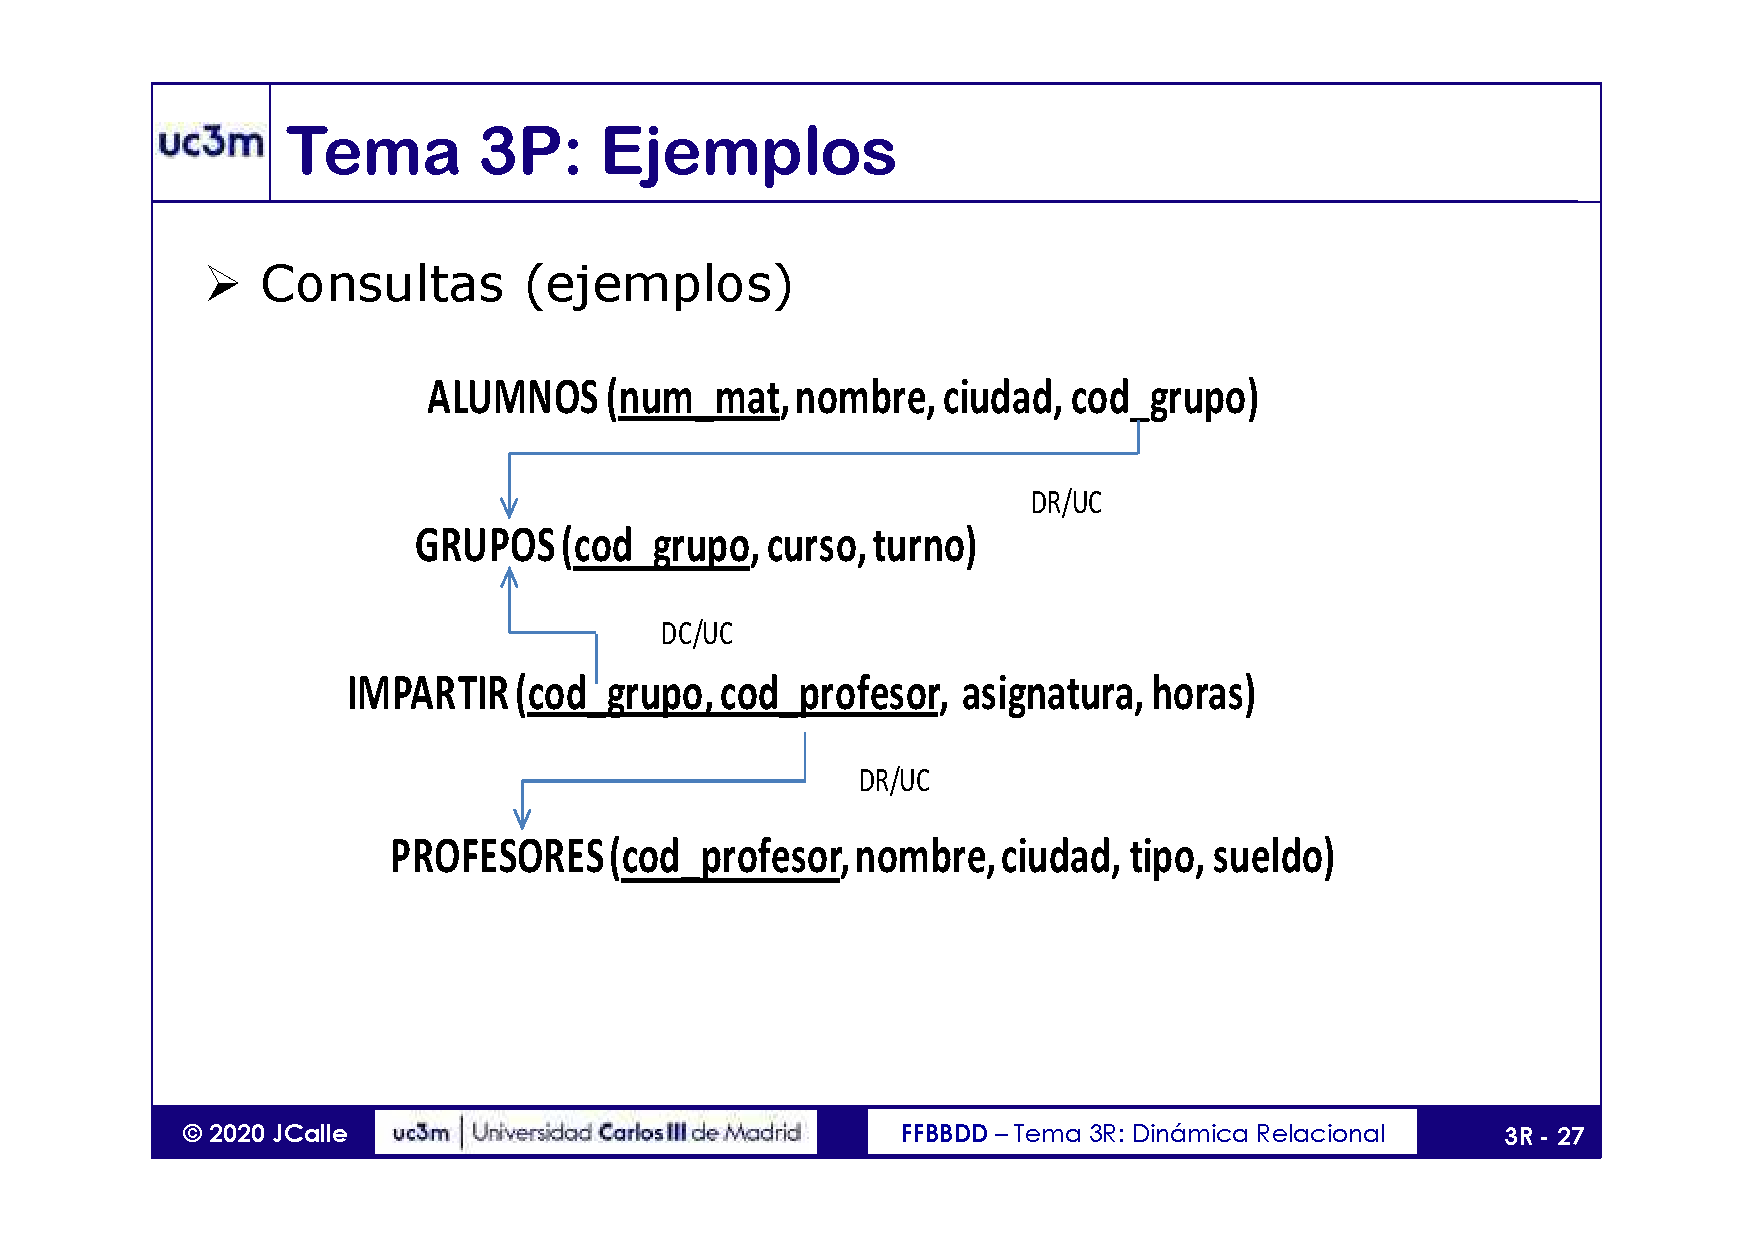
\includepdf[pages=-]{docs/ConsultasEnSQL.pdf}

\includepdf[pages=-]{docs/Practica_1_FBD.pdf}
\includepdf[pages=-]{docs/Presentacion_0_FBD.pdf}
\includepdf[pages=-]{docs/Presentacion_1_FBD.pdf}
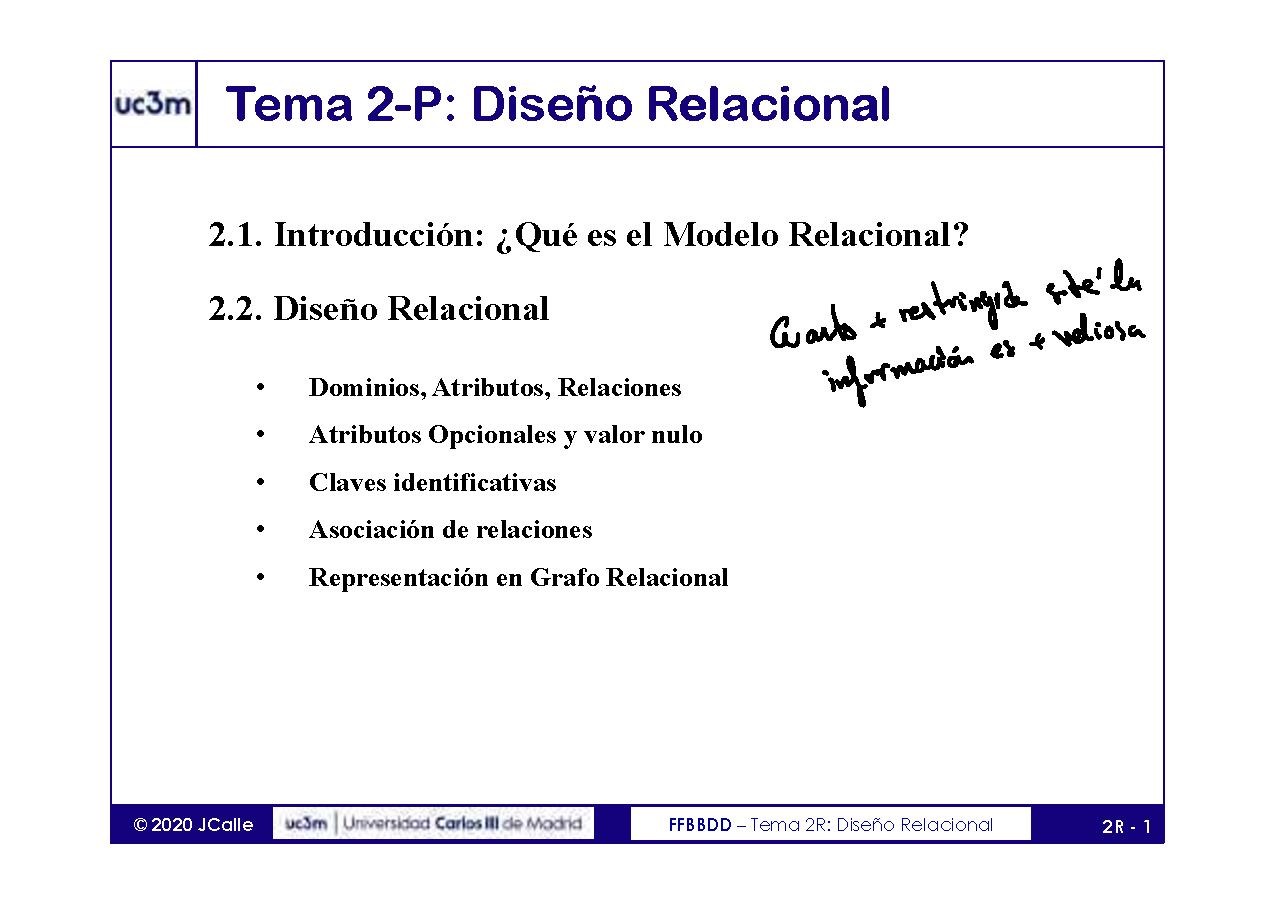
\includepdf[pages=-]{docs/Presentacion_2_Clase_FBD.pdf}
\includepdf[pages=-]{docs/Presentacion_2_FBD.pdf}
\includepdf[pages=-]{docs/Presentacion_3_clase_FBD.pdf}
\includepdf[pages=-]{docs/Presentacion_3_FBD.pdf}
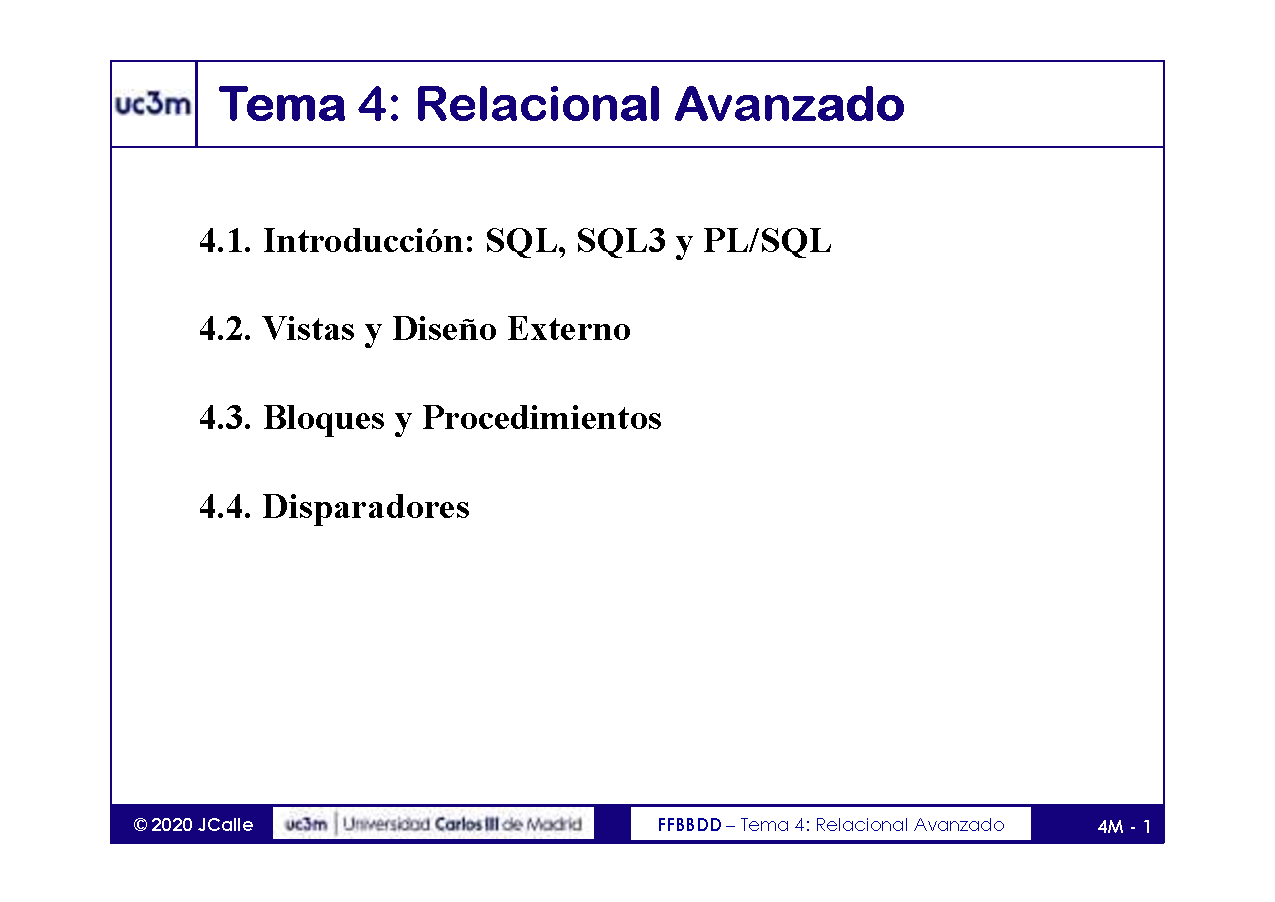
\includepdf[pages=-]{docs/Presentacion_4_FBD.pdf}
\includepdf[pages=-]{docs/Presentacion_5_FBD.pdf}
\includepdf[pages=-]{docs/Presentacion_6_FBD.pdf}
\includepdf[pages=-]{docs/Presentacion_7_FBD.pdf}

\part{Ejercicios}
\includepdf[pages=-]{docs/ff1.pdf}
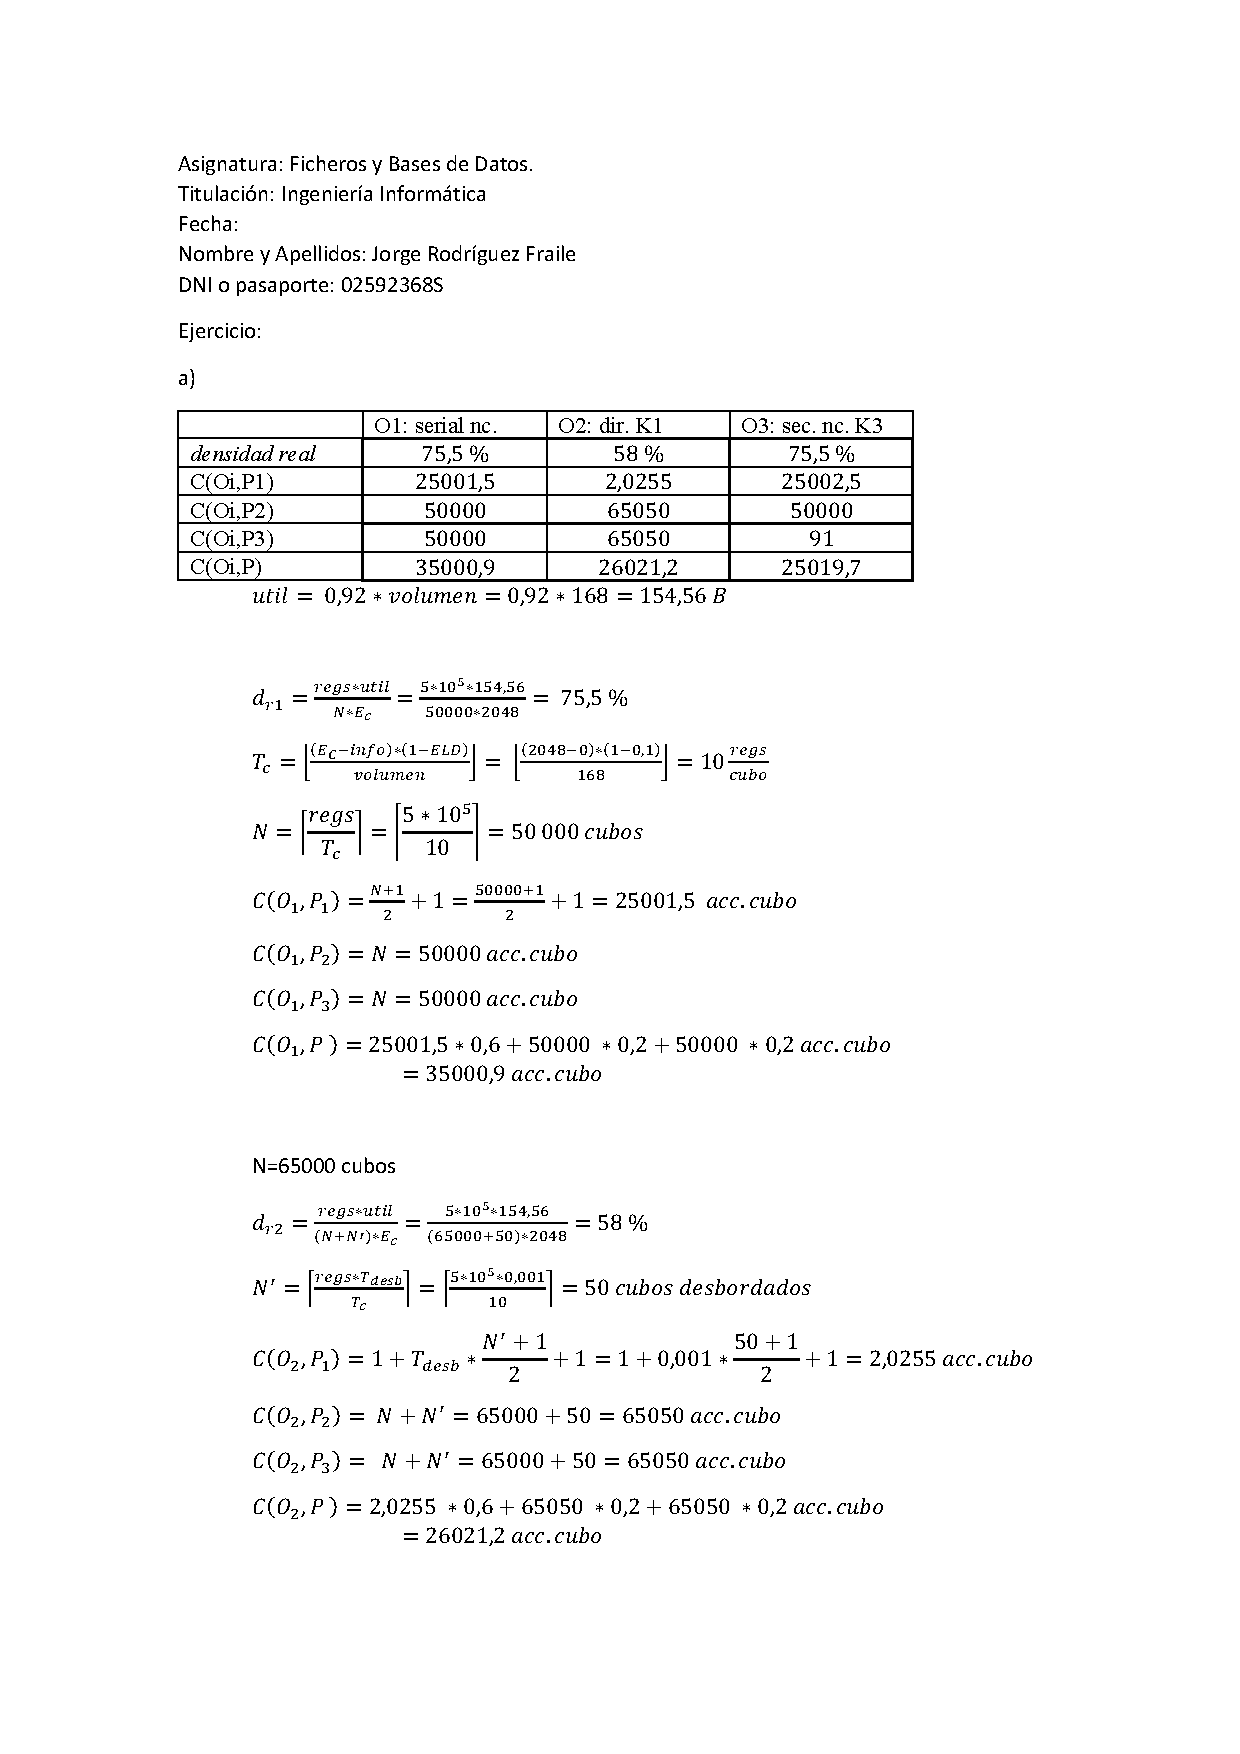
\includepdf[pages=-]{docs/ff3.pdf}
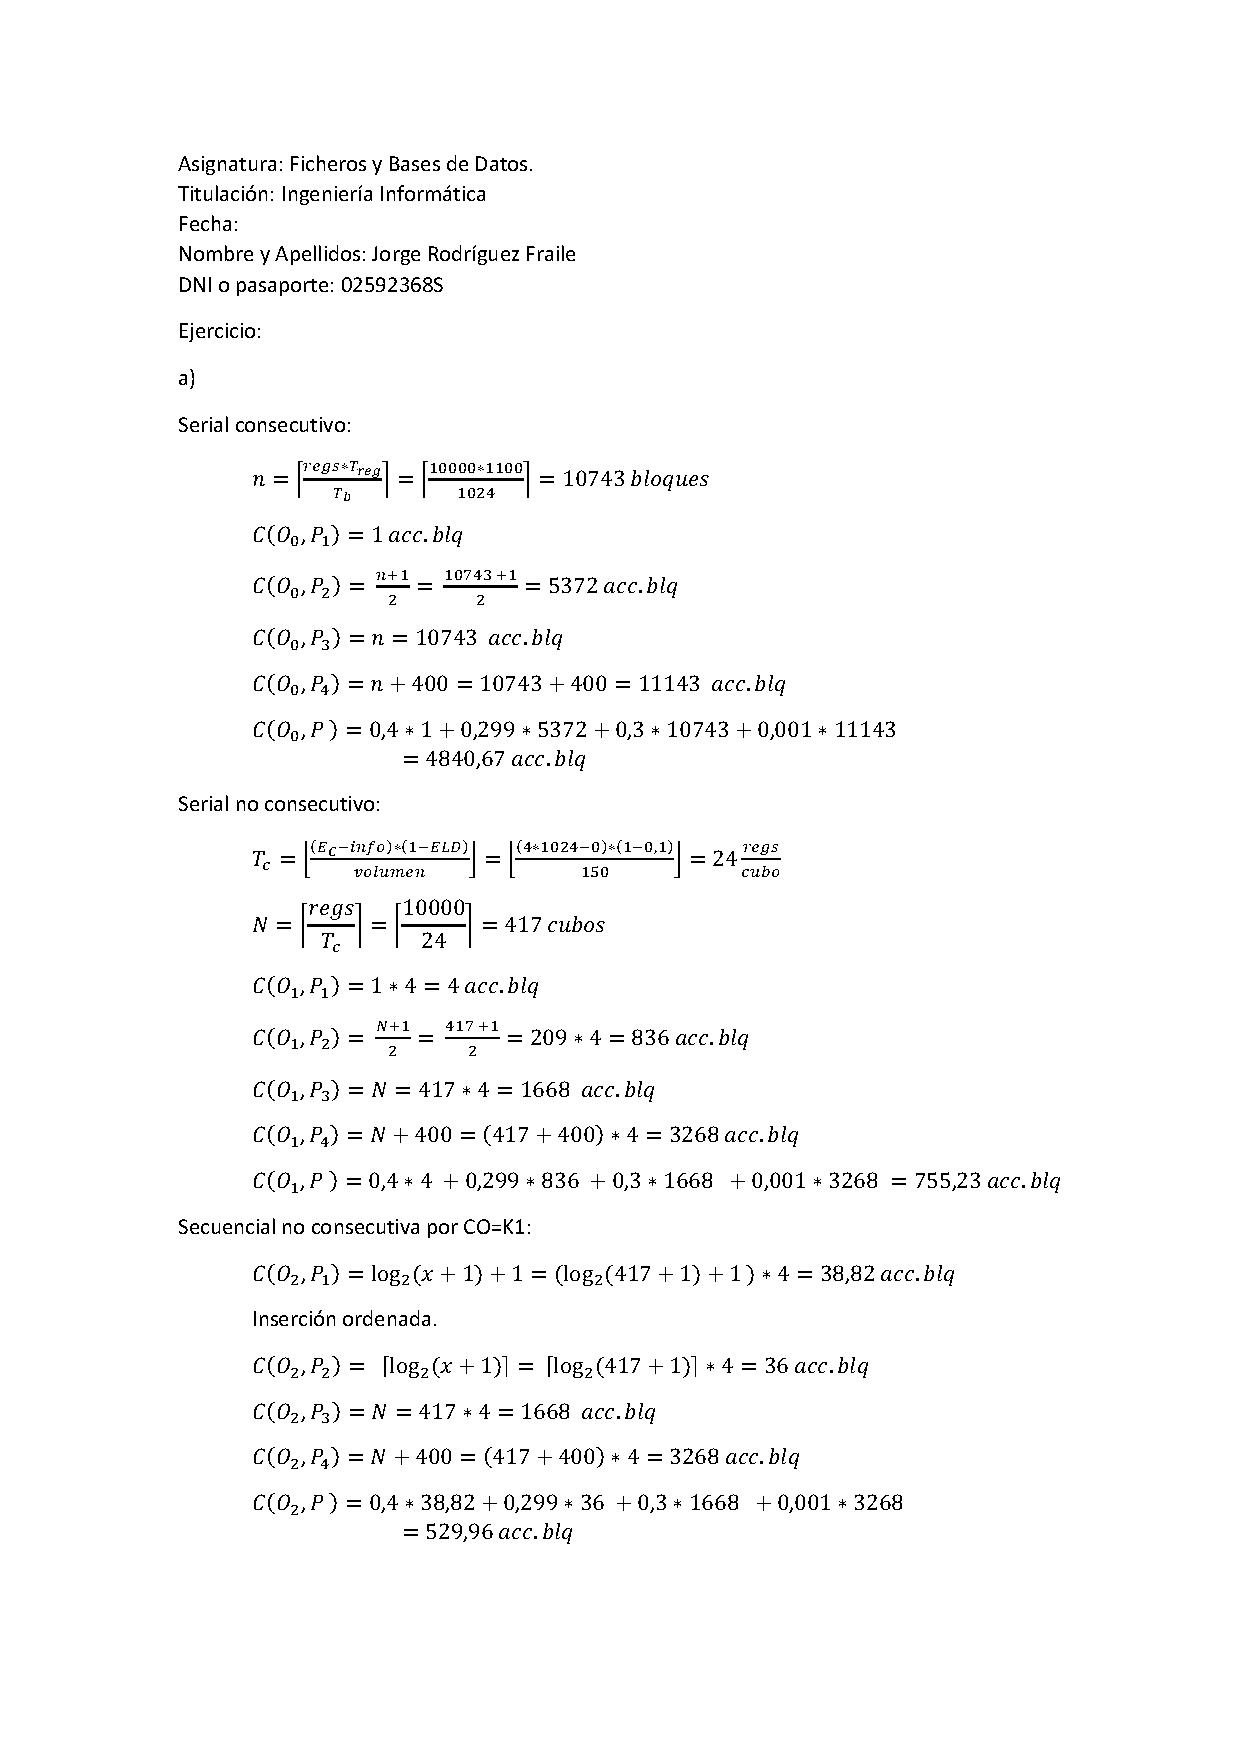
\includepdf[pages=-]{docs/ff4.pdf}
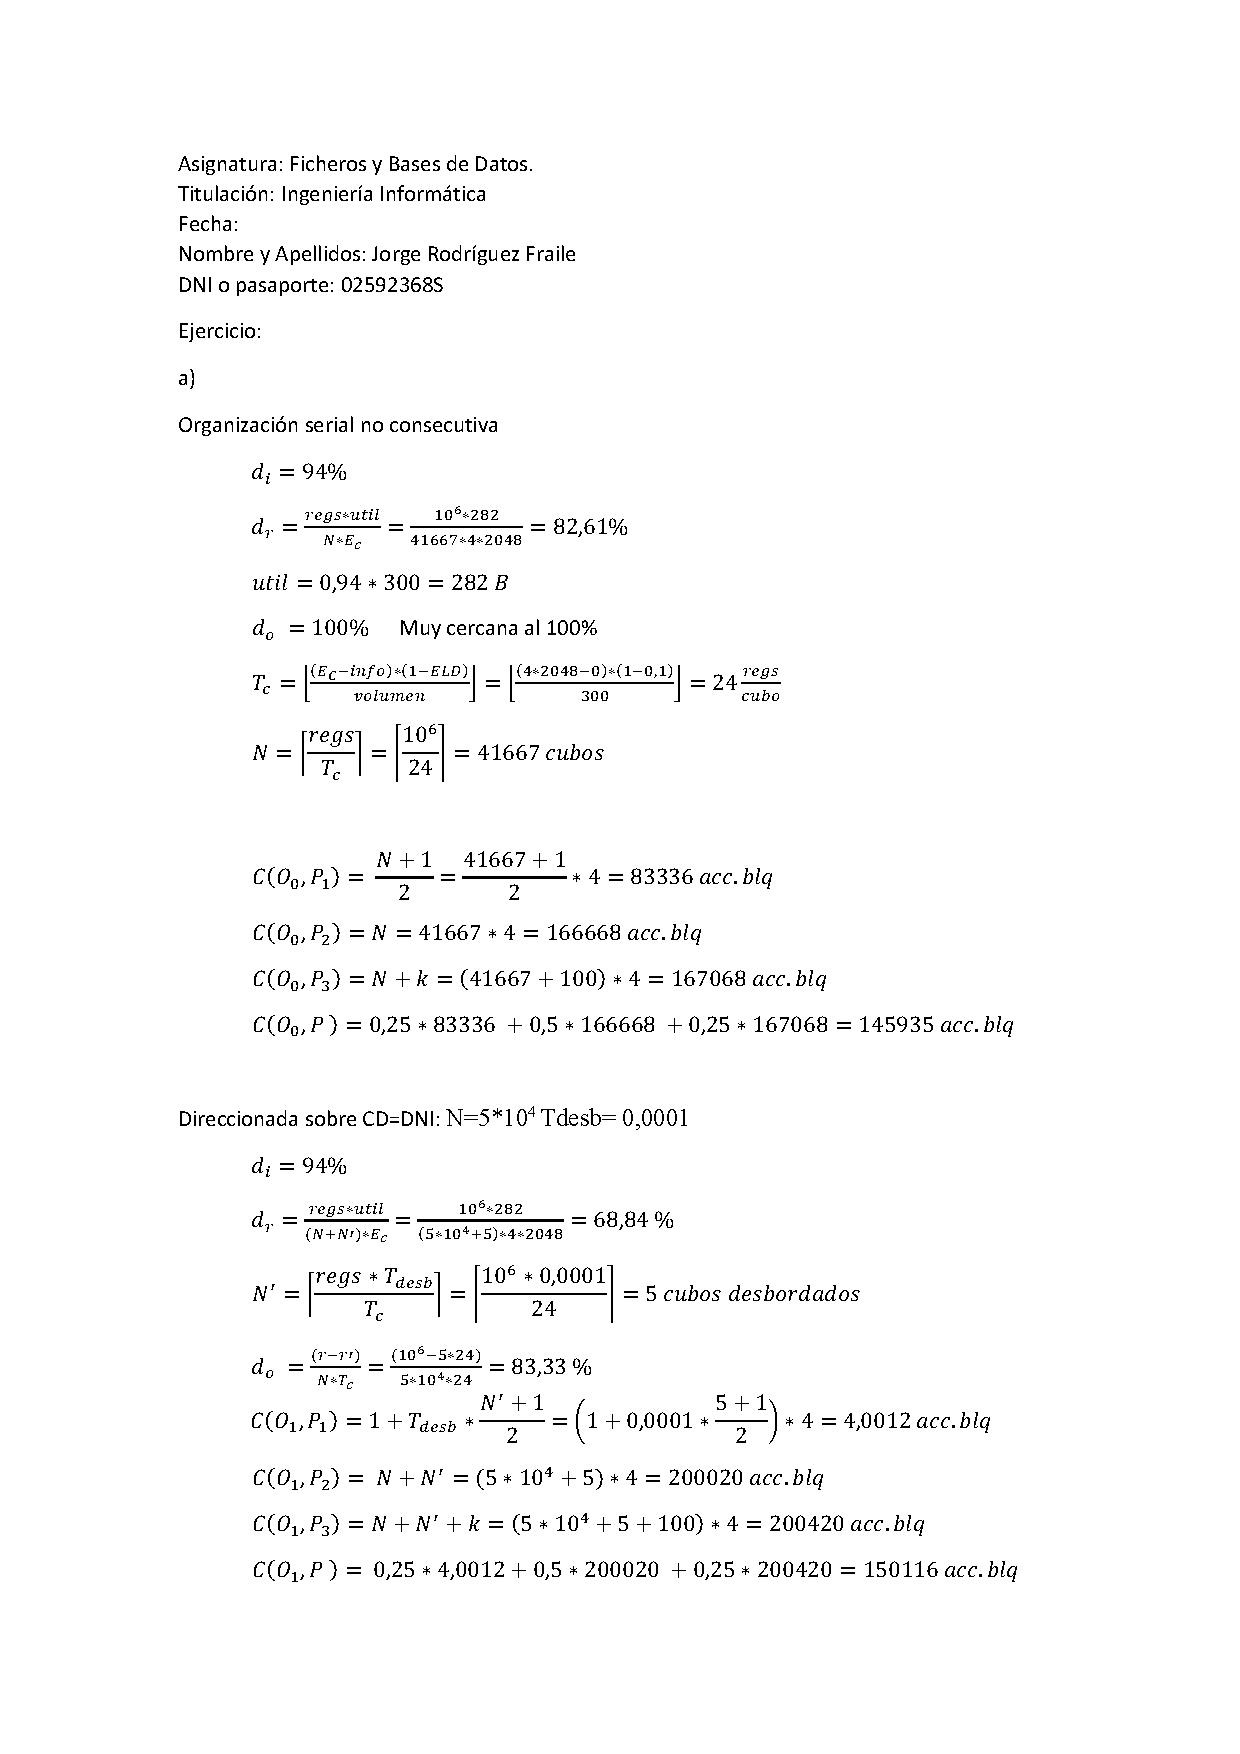
\includepdf[pages=-]{docs/ff5.pdf}
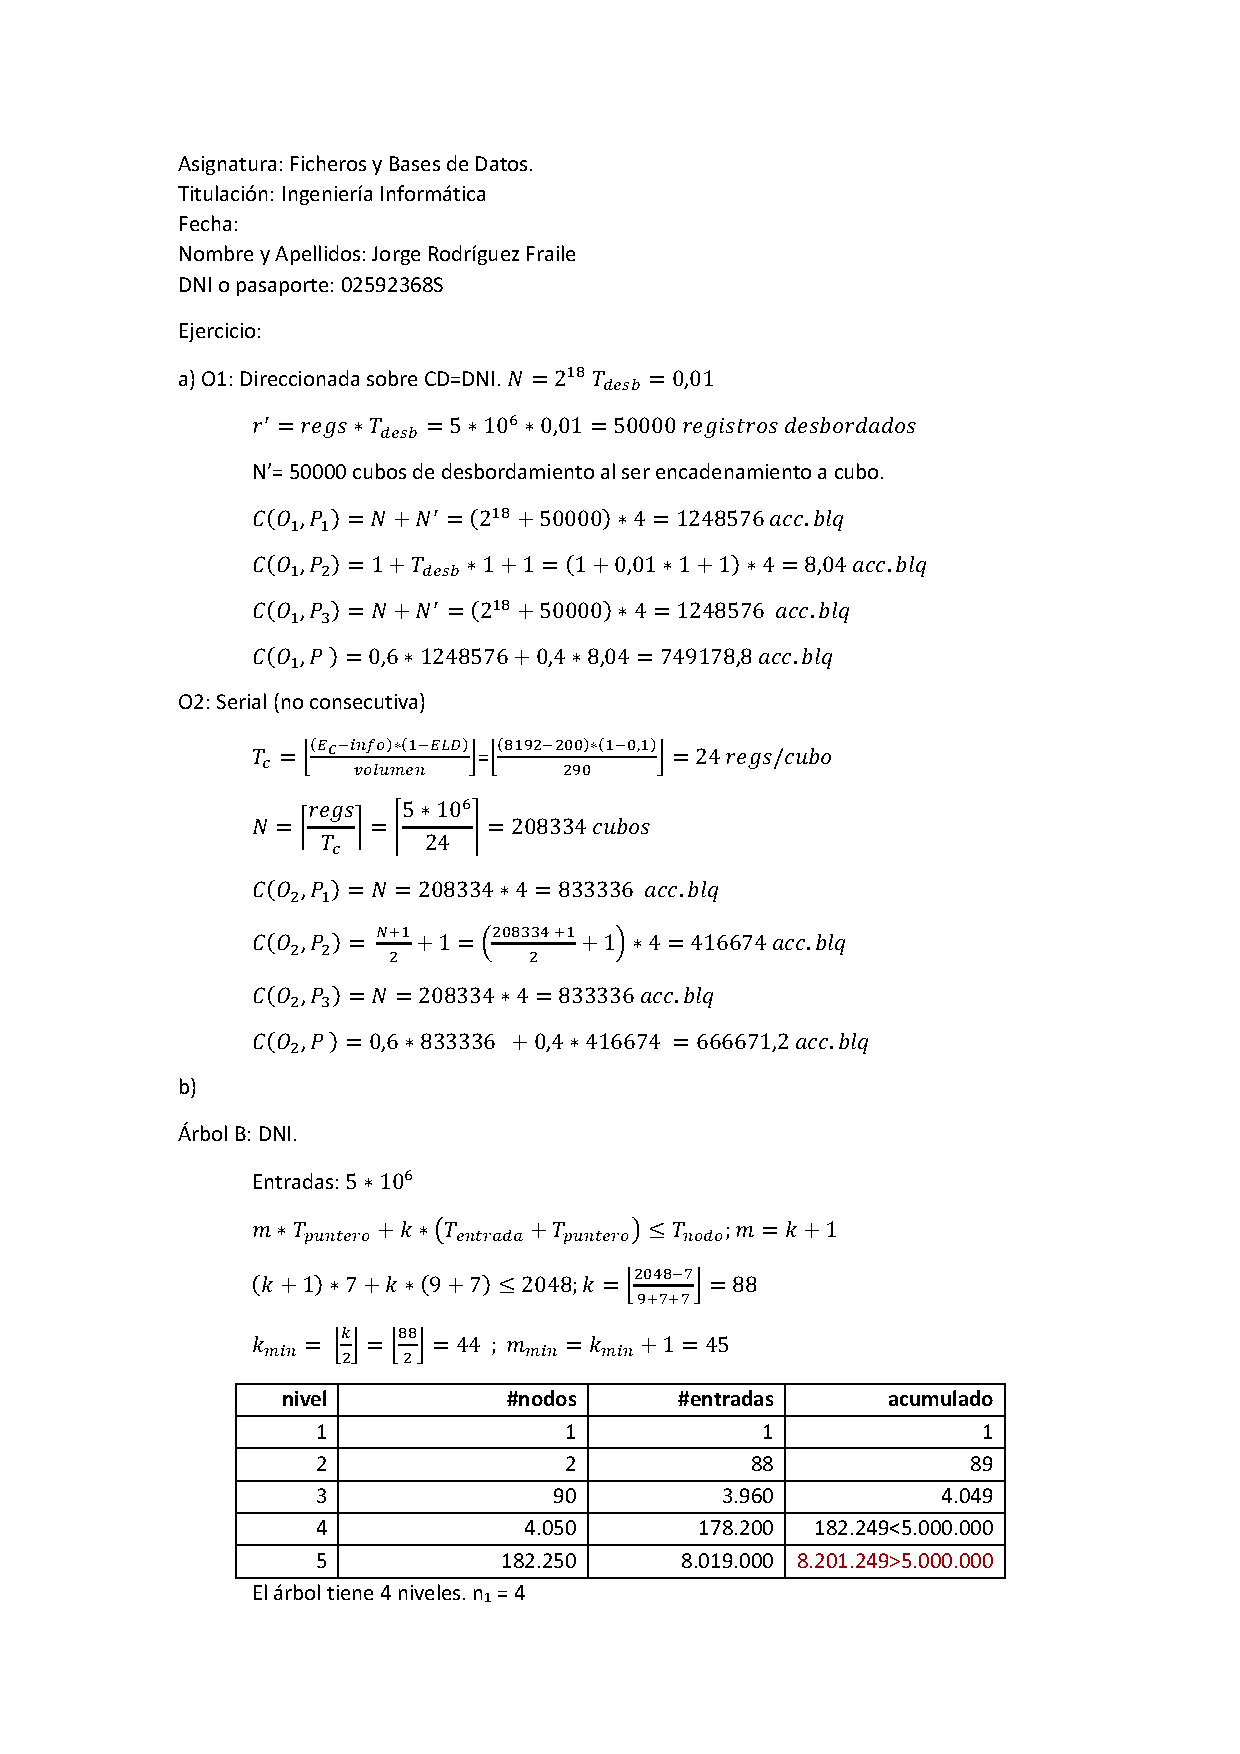
\includepdf[pages=-]{docs/ff6.pdf}
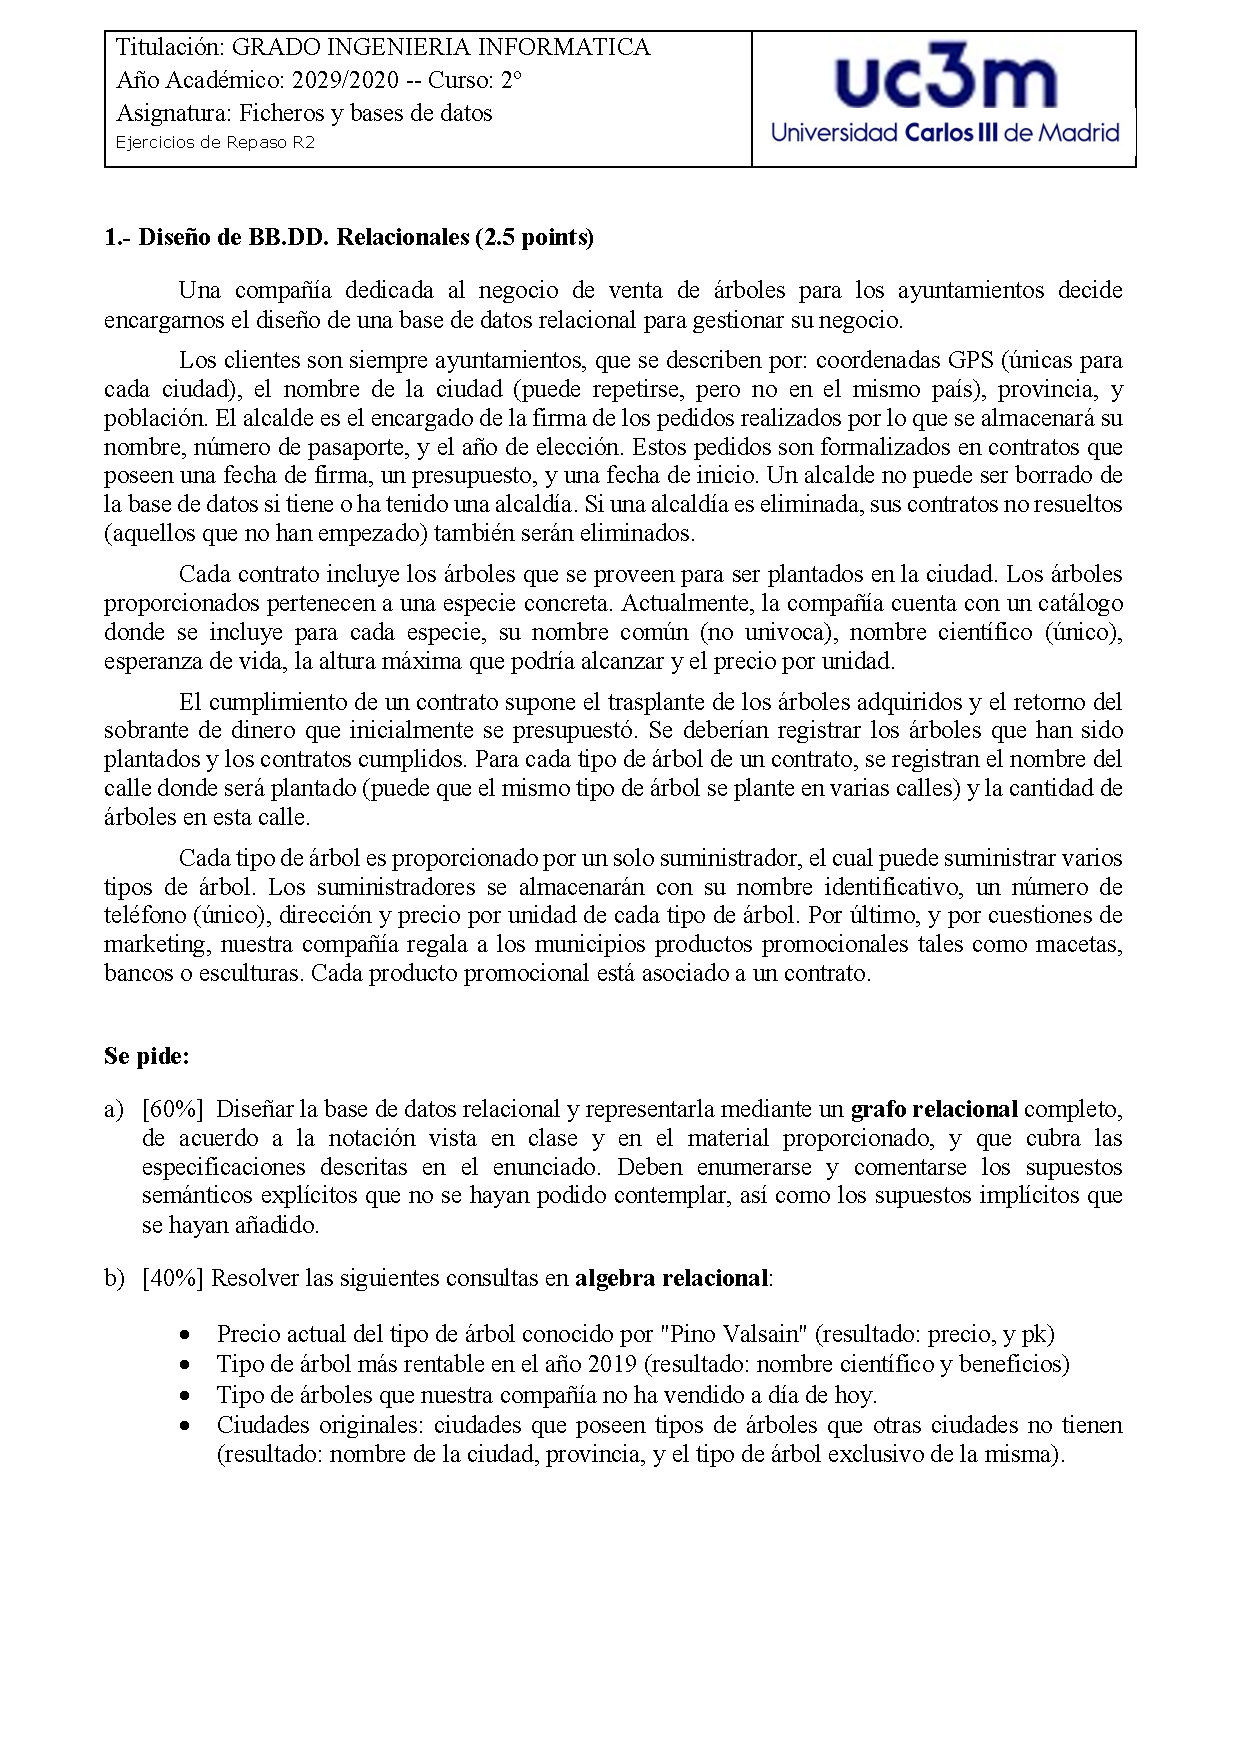
\includepdf[pages=-]{docs/repaso_3.pdf}
\includepdf[pages=-]{docs/Repaso_28-5.pdf}
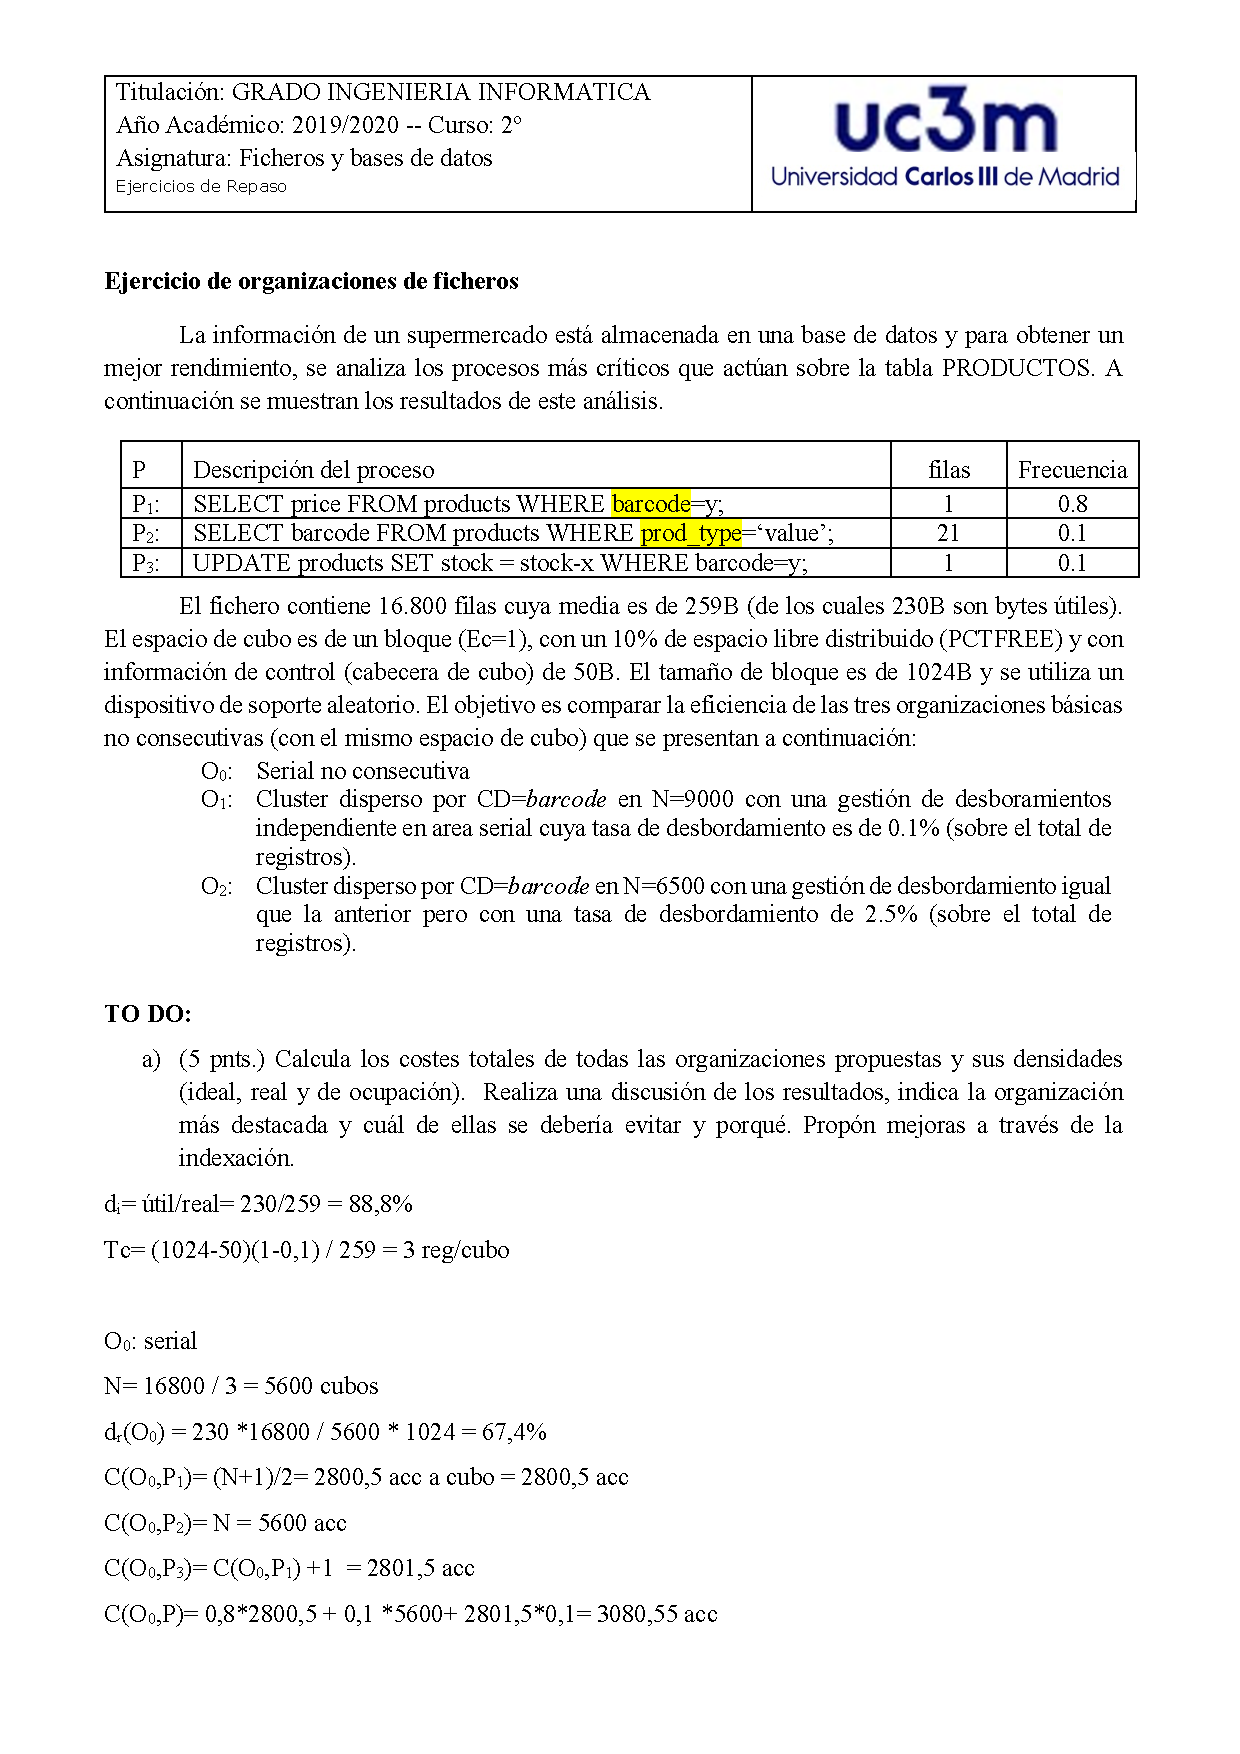
\includepdf[pages=-]{docs/repaso1_sol.pdf}
\includepdf[pages=-]{docs/repaso1.pdf}
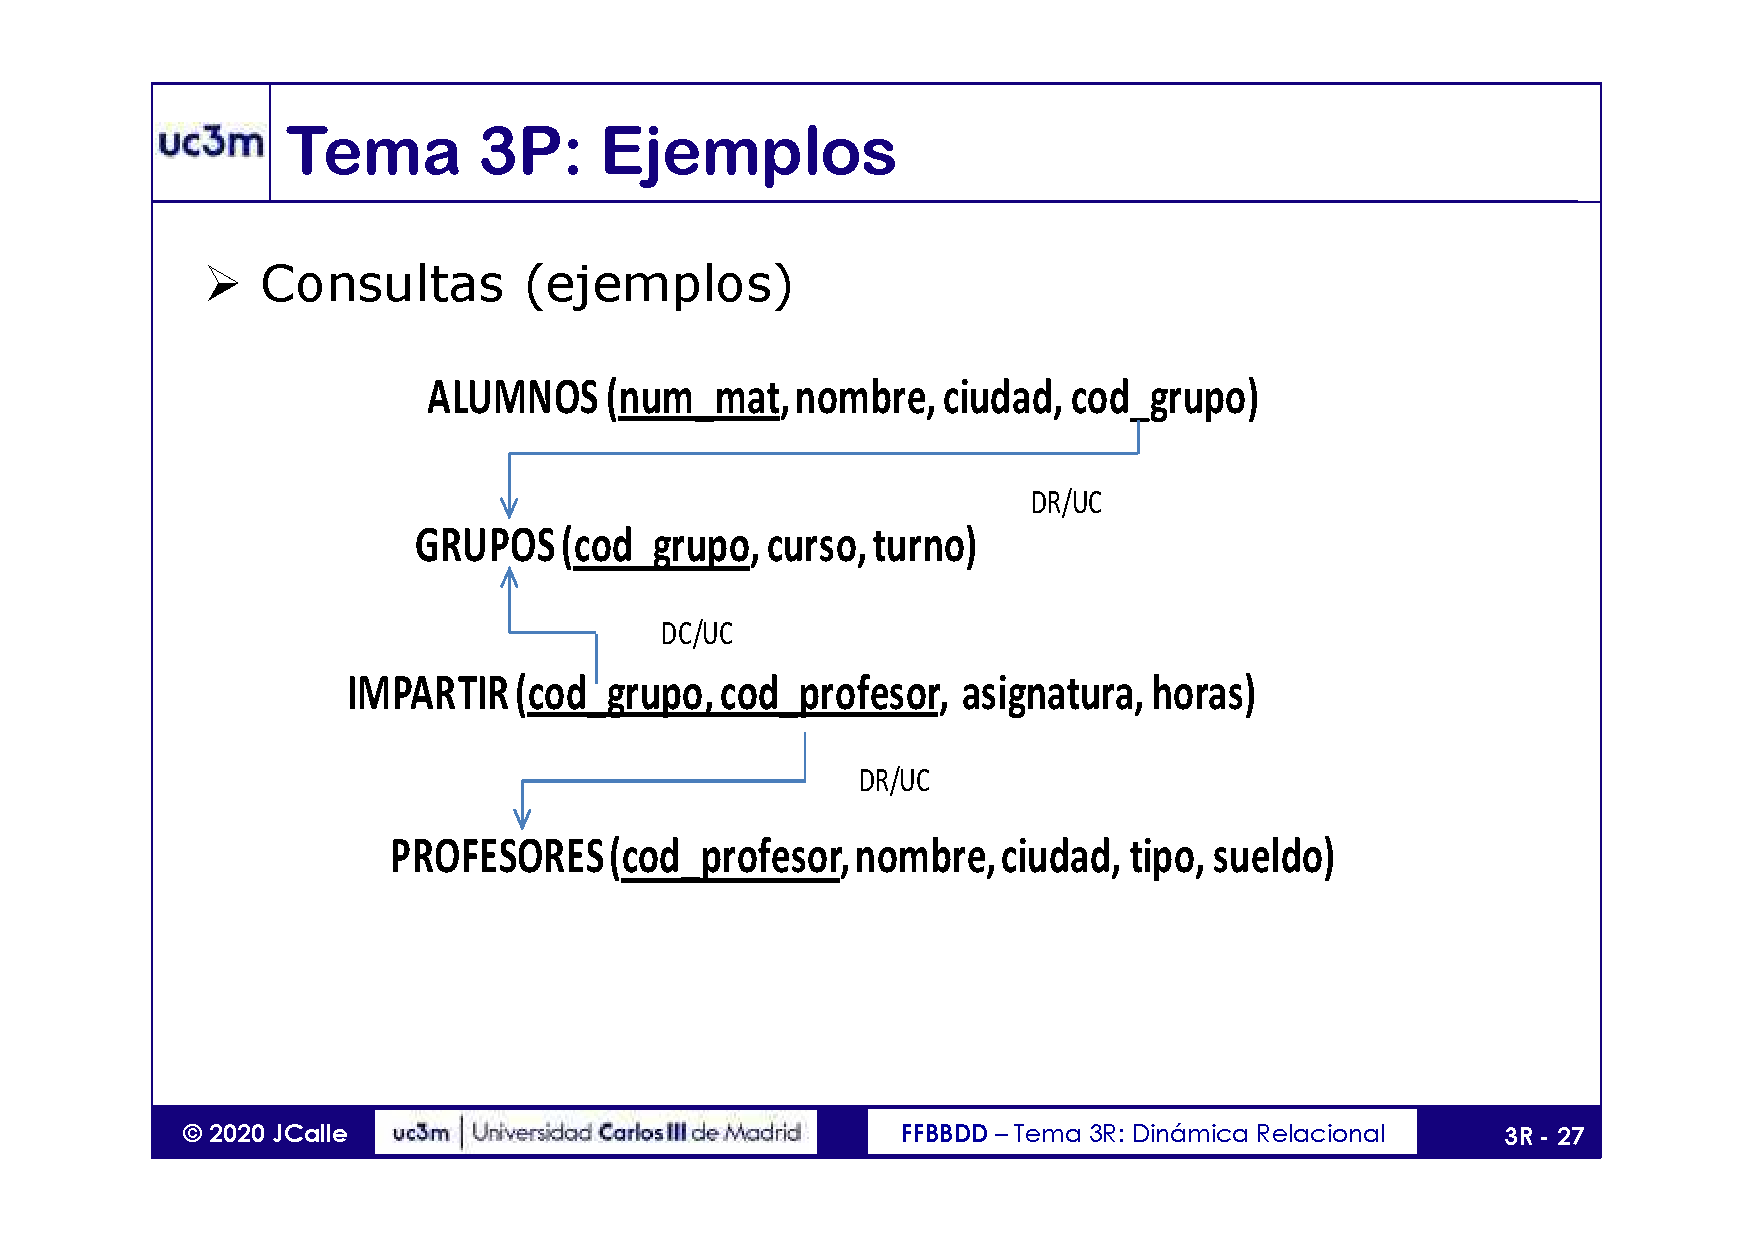
\includepdf[pages=-]{docs/ConsultasEnSQL.pdf}
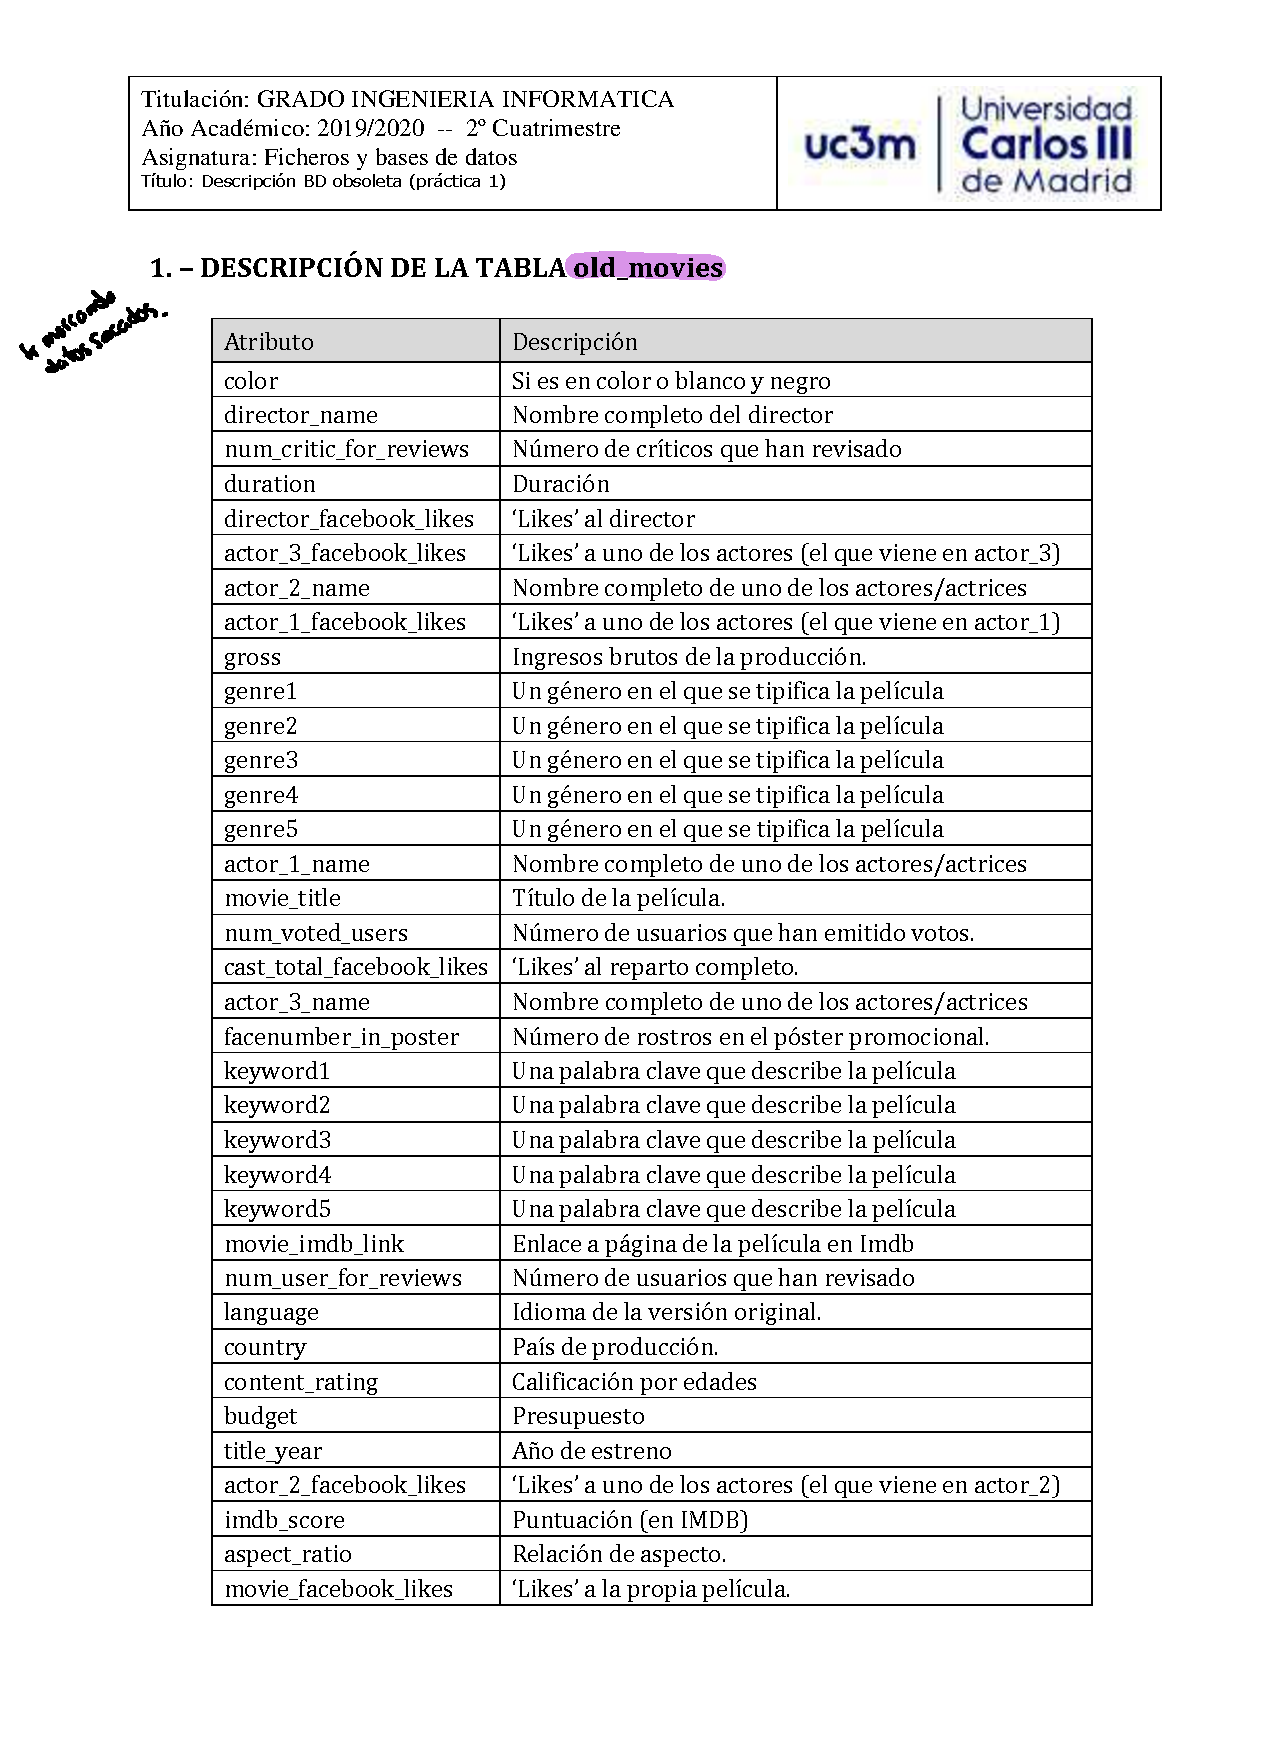
\includepdf[pages=-]{docs/Descripcion_datos_practica_1_FBD.pdf}
\includepdf[pages=-]{docs/Ejercicio_Ficheros_1_FBD.pdf}
\includepdf[pages=-]{docs/Ejercicio_Ficheros_1_Solucion_FBD.pdf}
\includepdf[pages=-]{docs/Ejercicio_Ficheros_2_FBD.pdf}
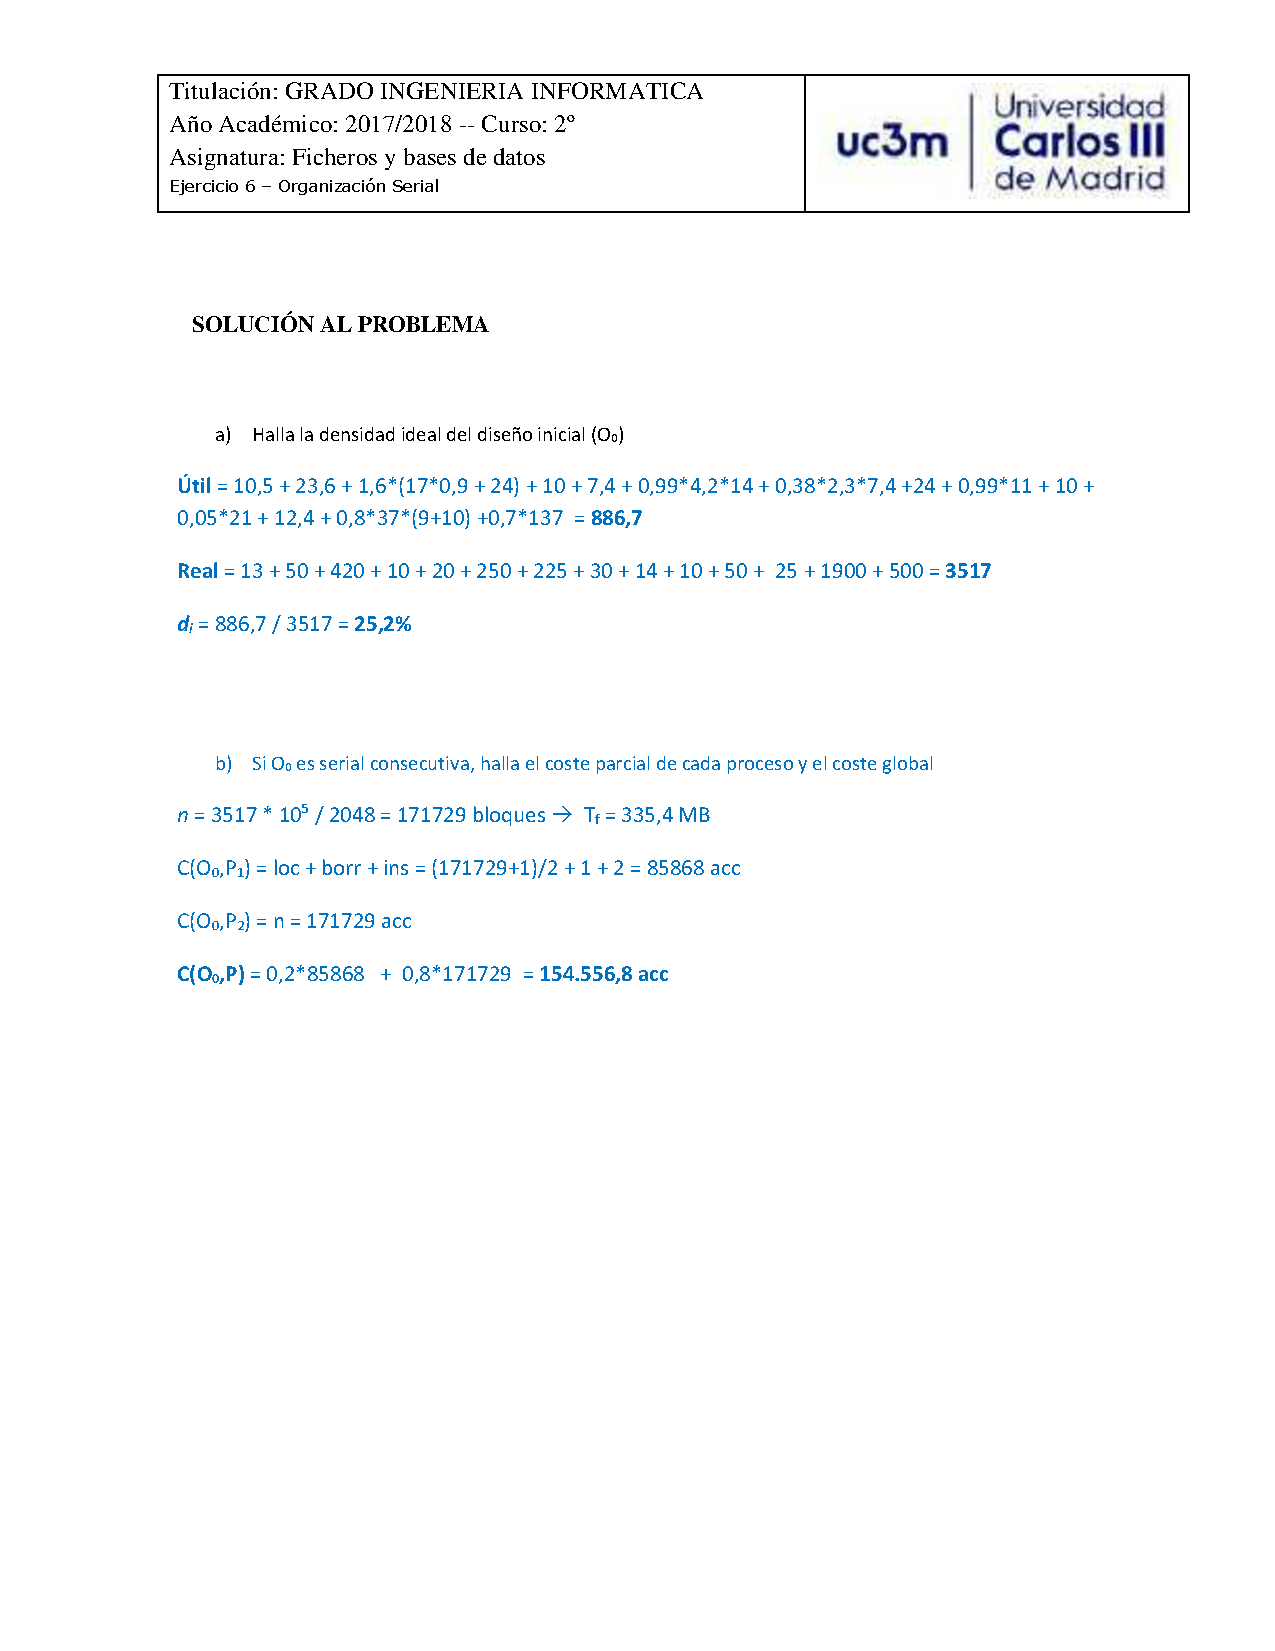
\includepdf[pages=-]{docs/Ejercicio_Ficheros_2_Solucion_FBD.pdf}
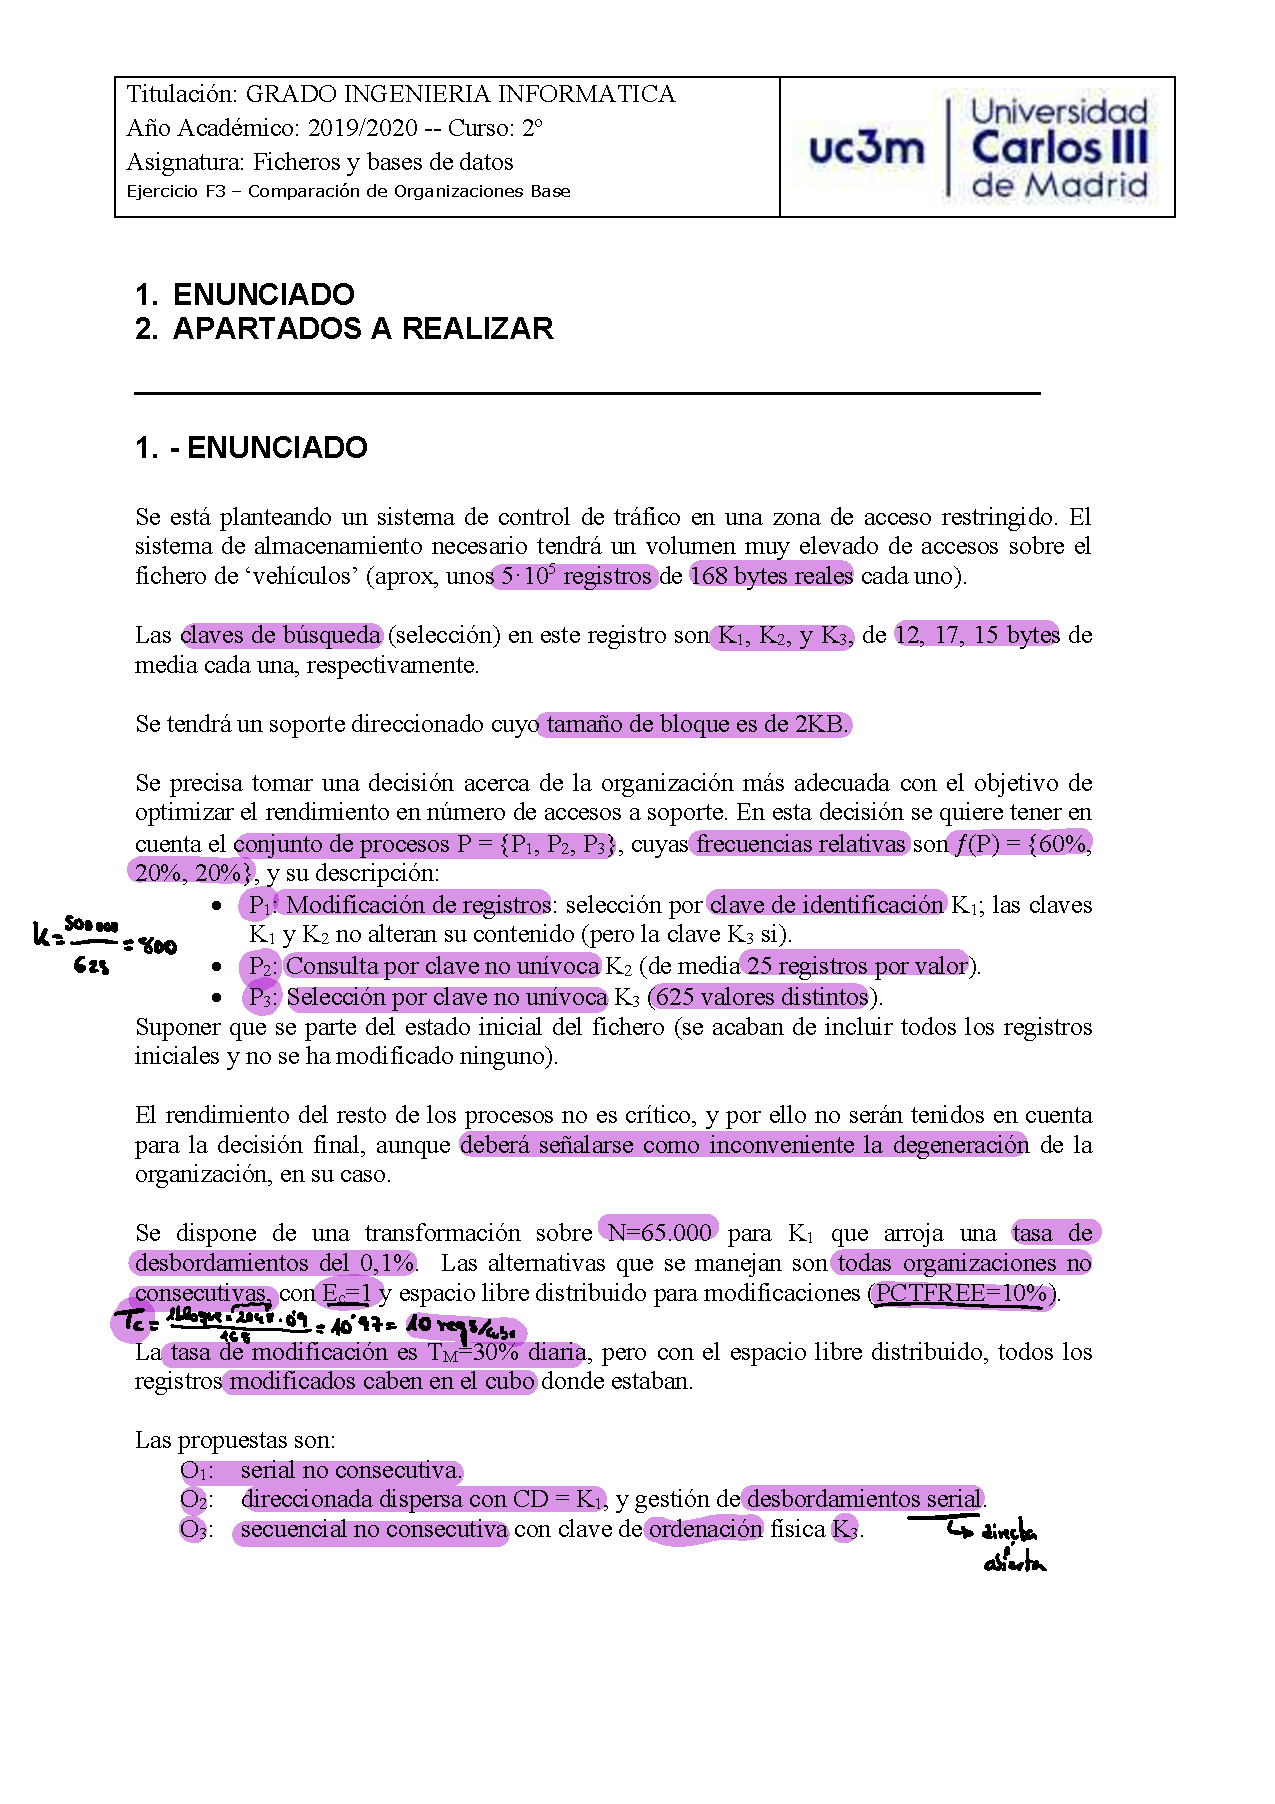
\includepdf[pages=-]{docs/Ejercicio_Ficheros_3_FBD.pdf}
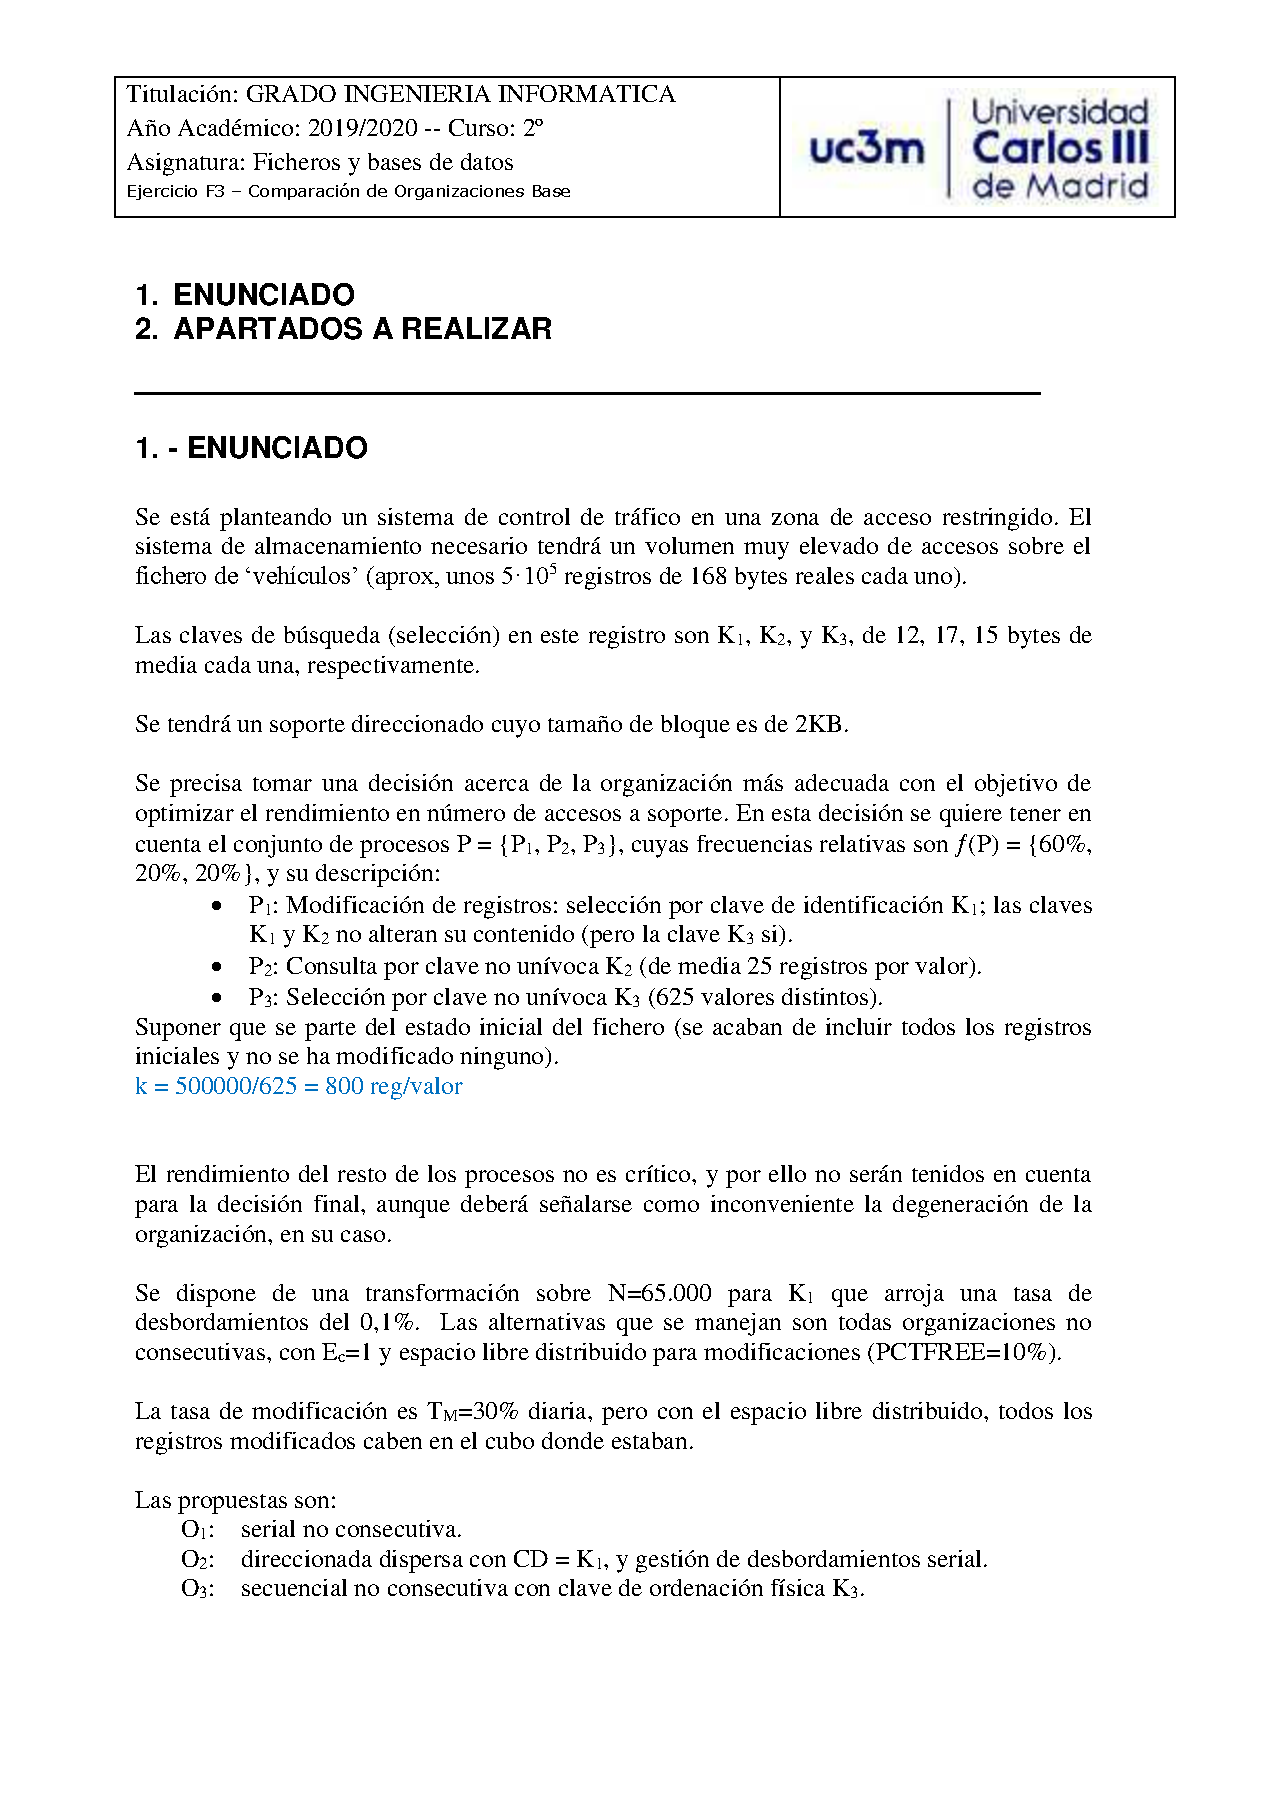
\includepdf[pages=-]{docs/Ejercicio_Ficheros_3_Solucion_FBD.pdf}
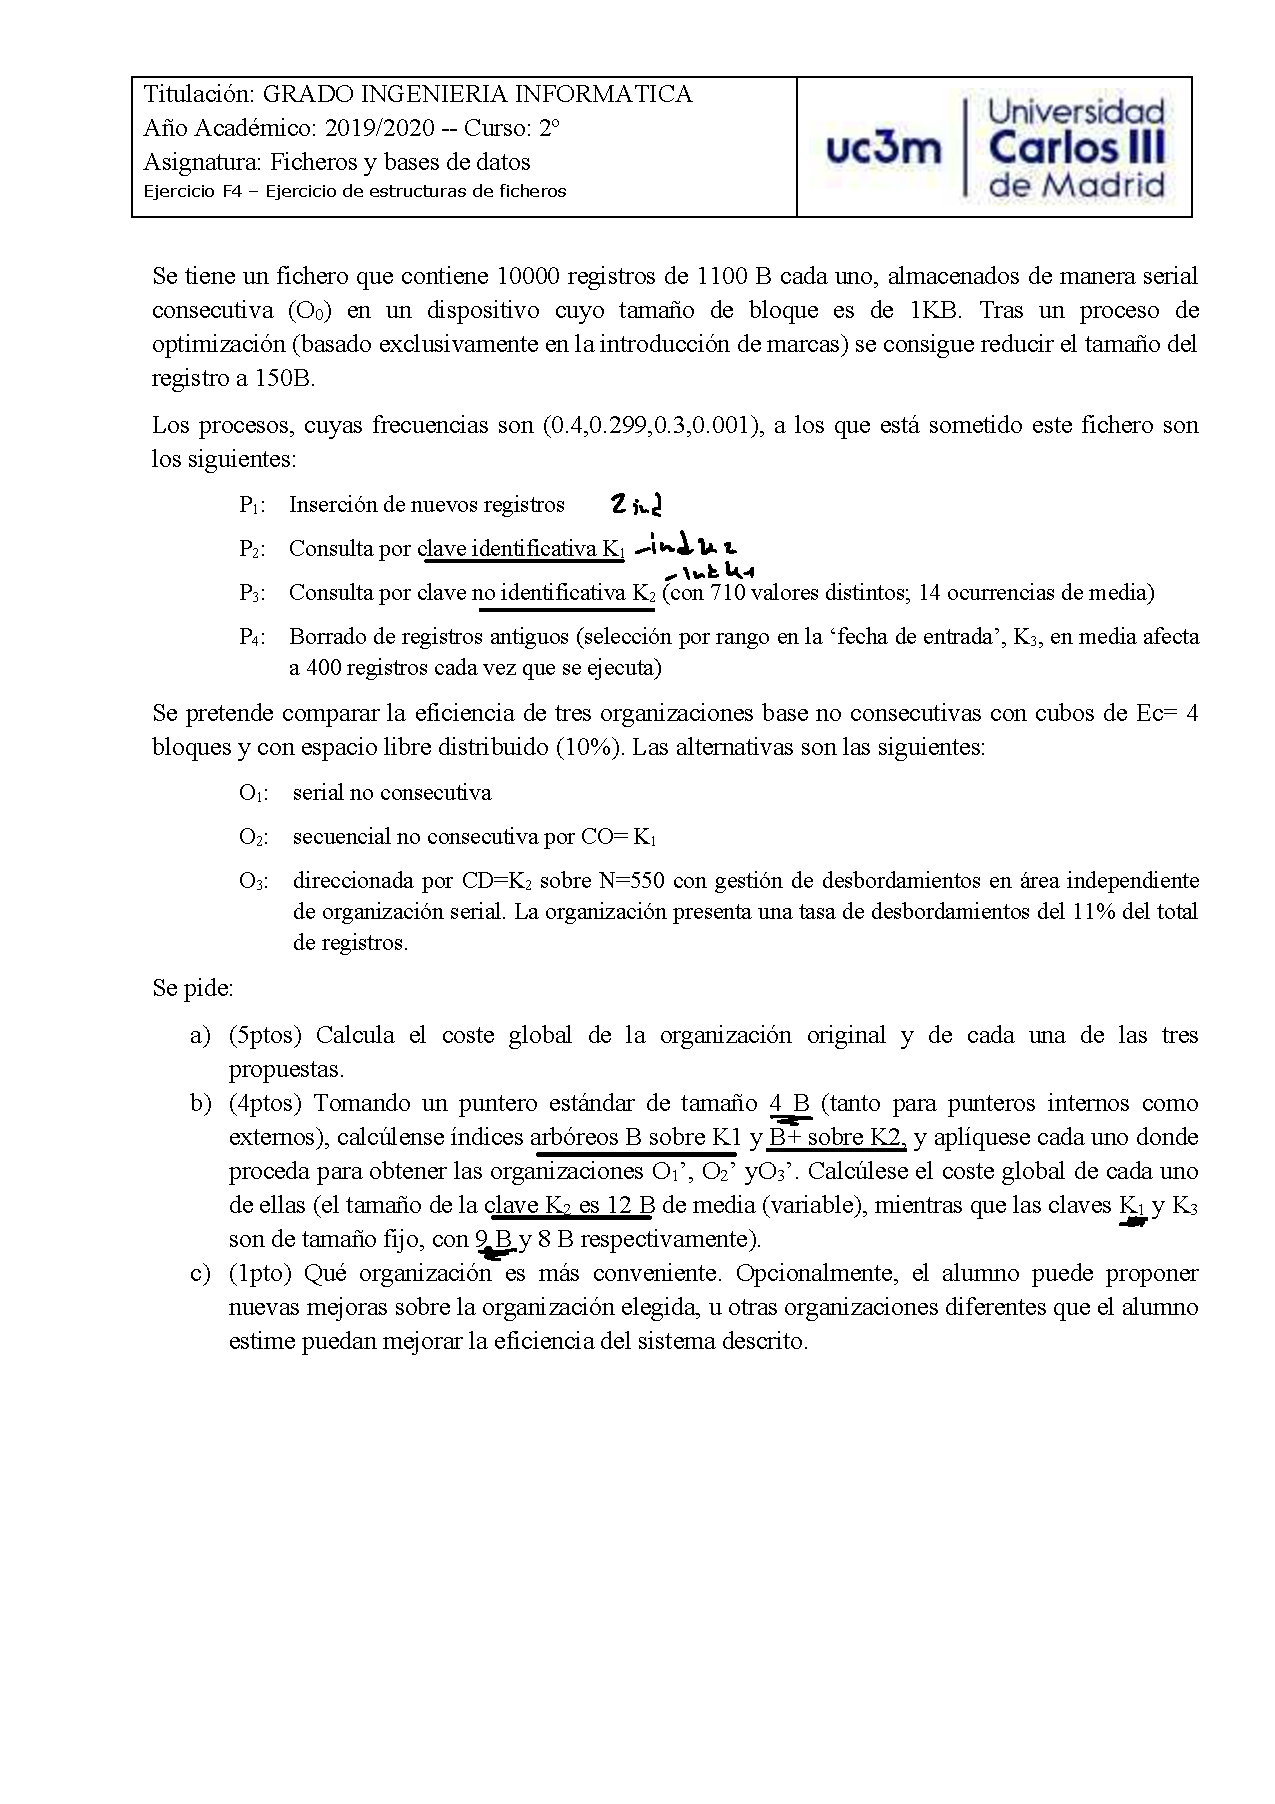
\includepdf[pages=-]{docs/Ejercicio_Ficheros_4_FBD.pdf}
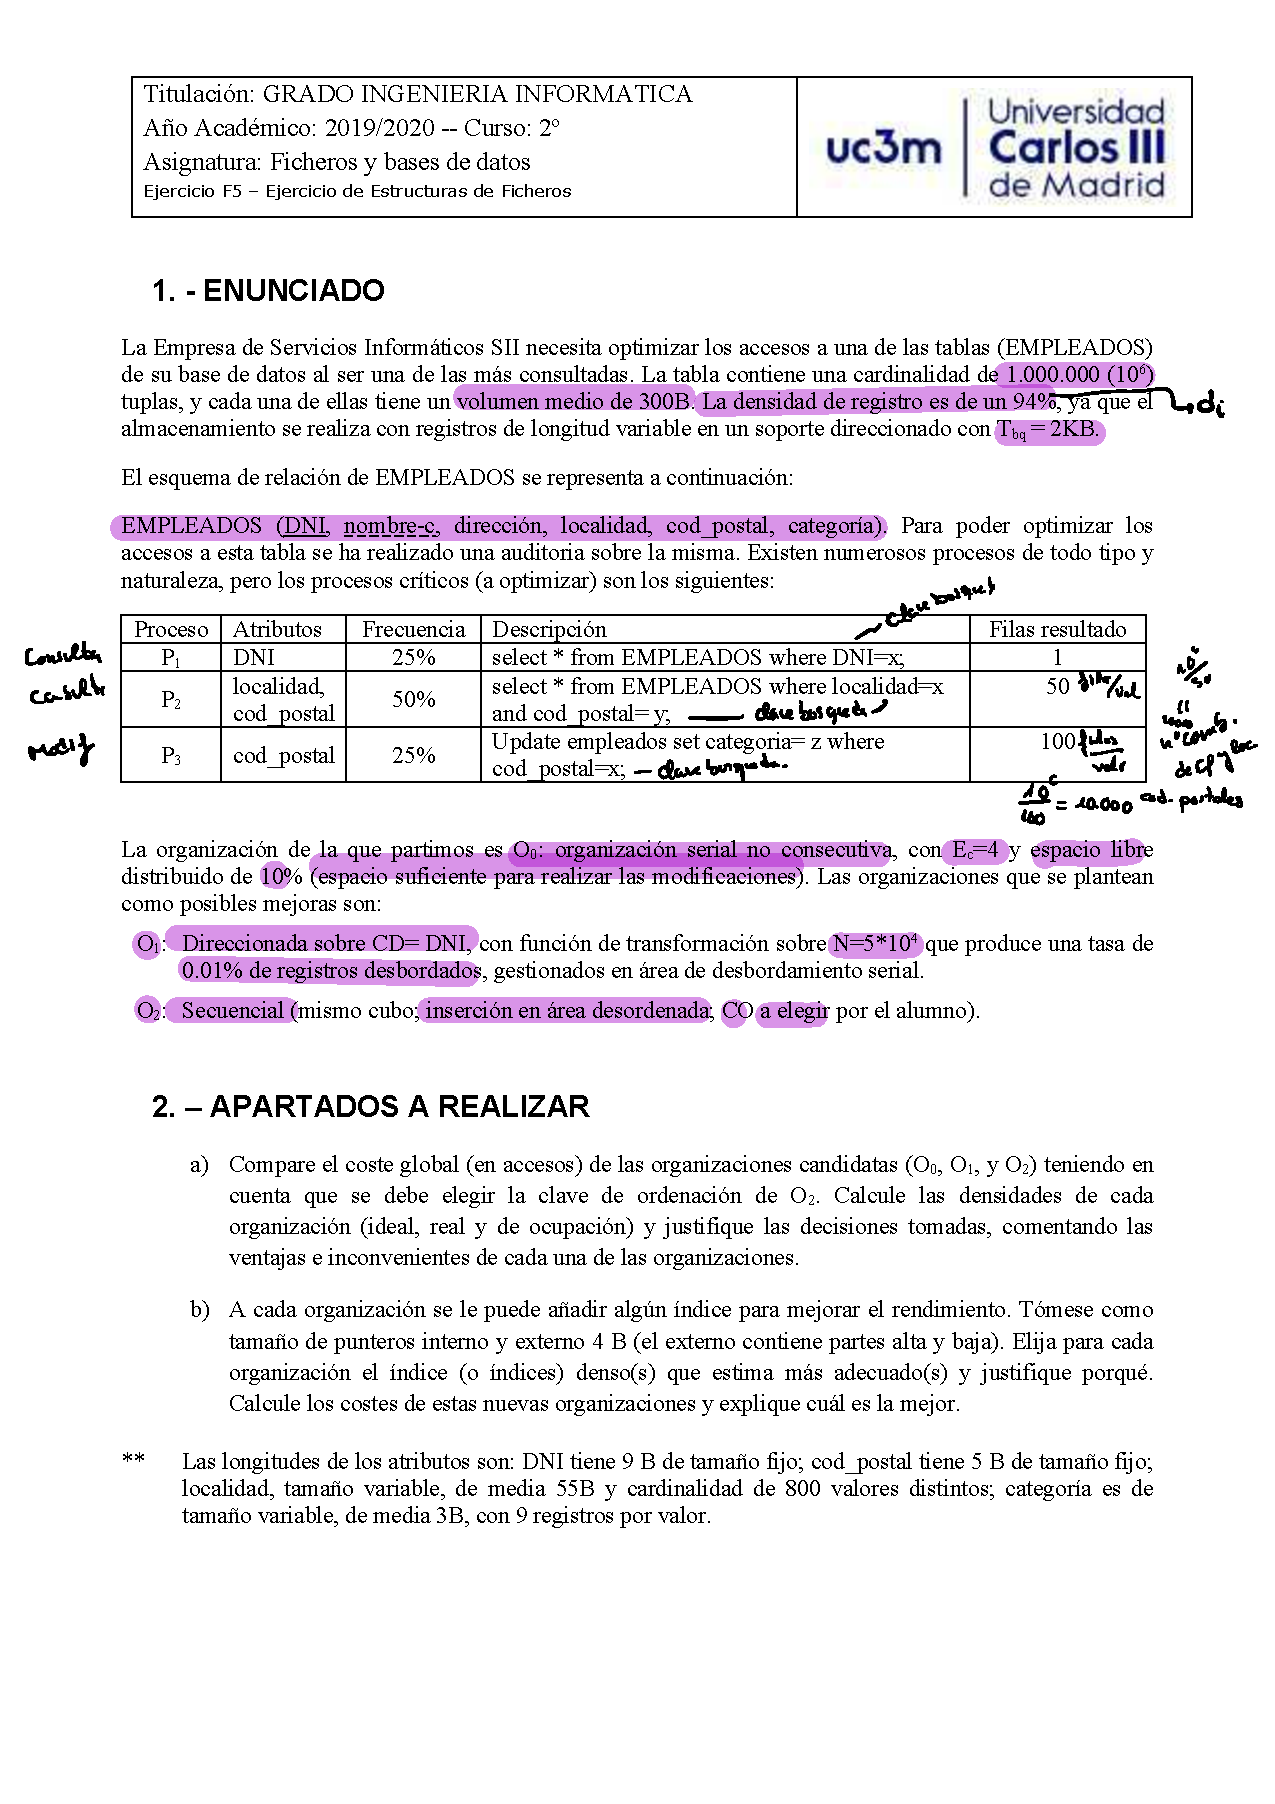
\includepdf[pages=-]{docs/Ejercicio_Ficheros_5_FBD.pdf}
\includepdf[pages=-]{docs/Ejercicio_Ficheros_6_FBD.pdf}
\includepdf[pages=-]{docs/Ejercicios_Tema_3_y_Extras_del_Cafe.pdf}
\includepdf[pages=-]{docs/Enunciado_Practica_1_FBD.pdf}
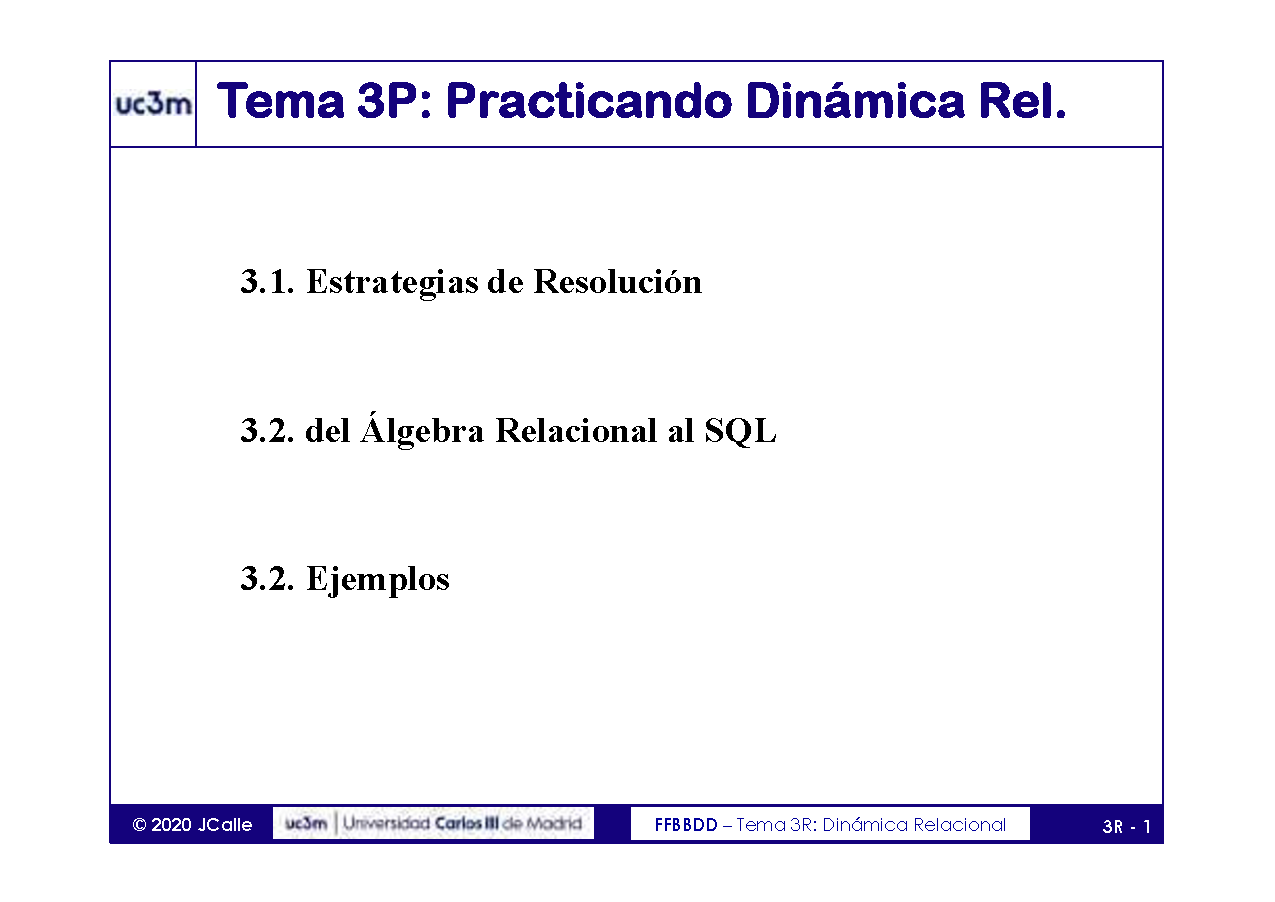
\includepdf[pages=-]{docs/GI_FFBBDD_tema3P_sol.pdf}
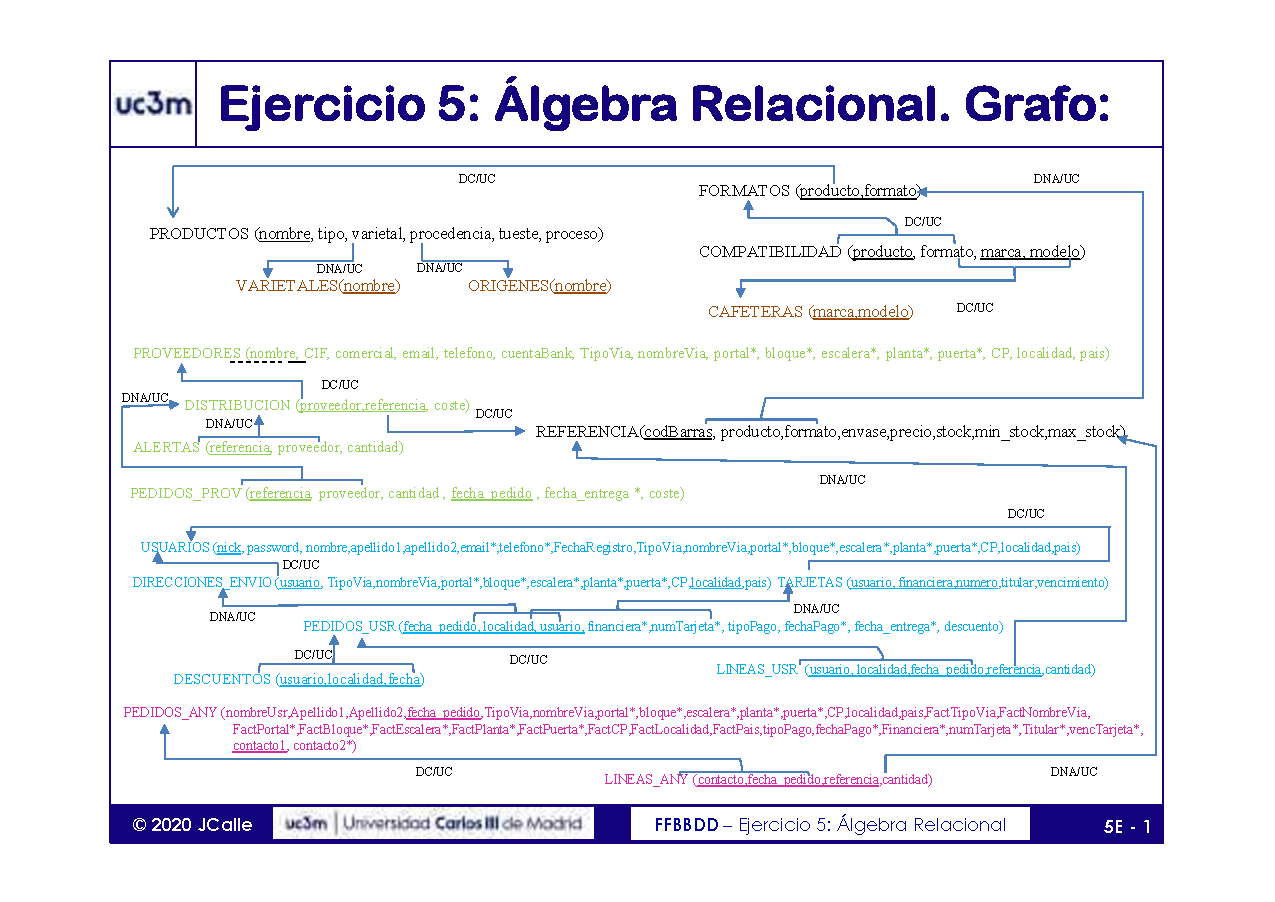
\includepdf[pages=-]{docs/GI_FFBBDD_ejercicio_5_sol_completa.pdf}
\includepdf[pages=-]{docs/GI_FFBBDD_ejercicio_ficheros_extra_solucion.pdf}
\includepdf[pages=-]{docs/Laboratorio_2_FBD.pdf}
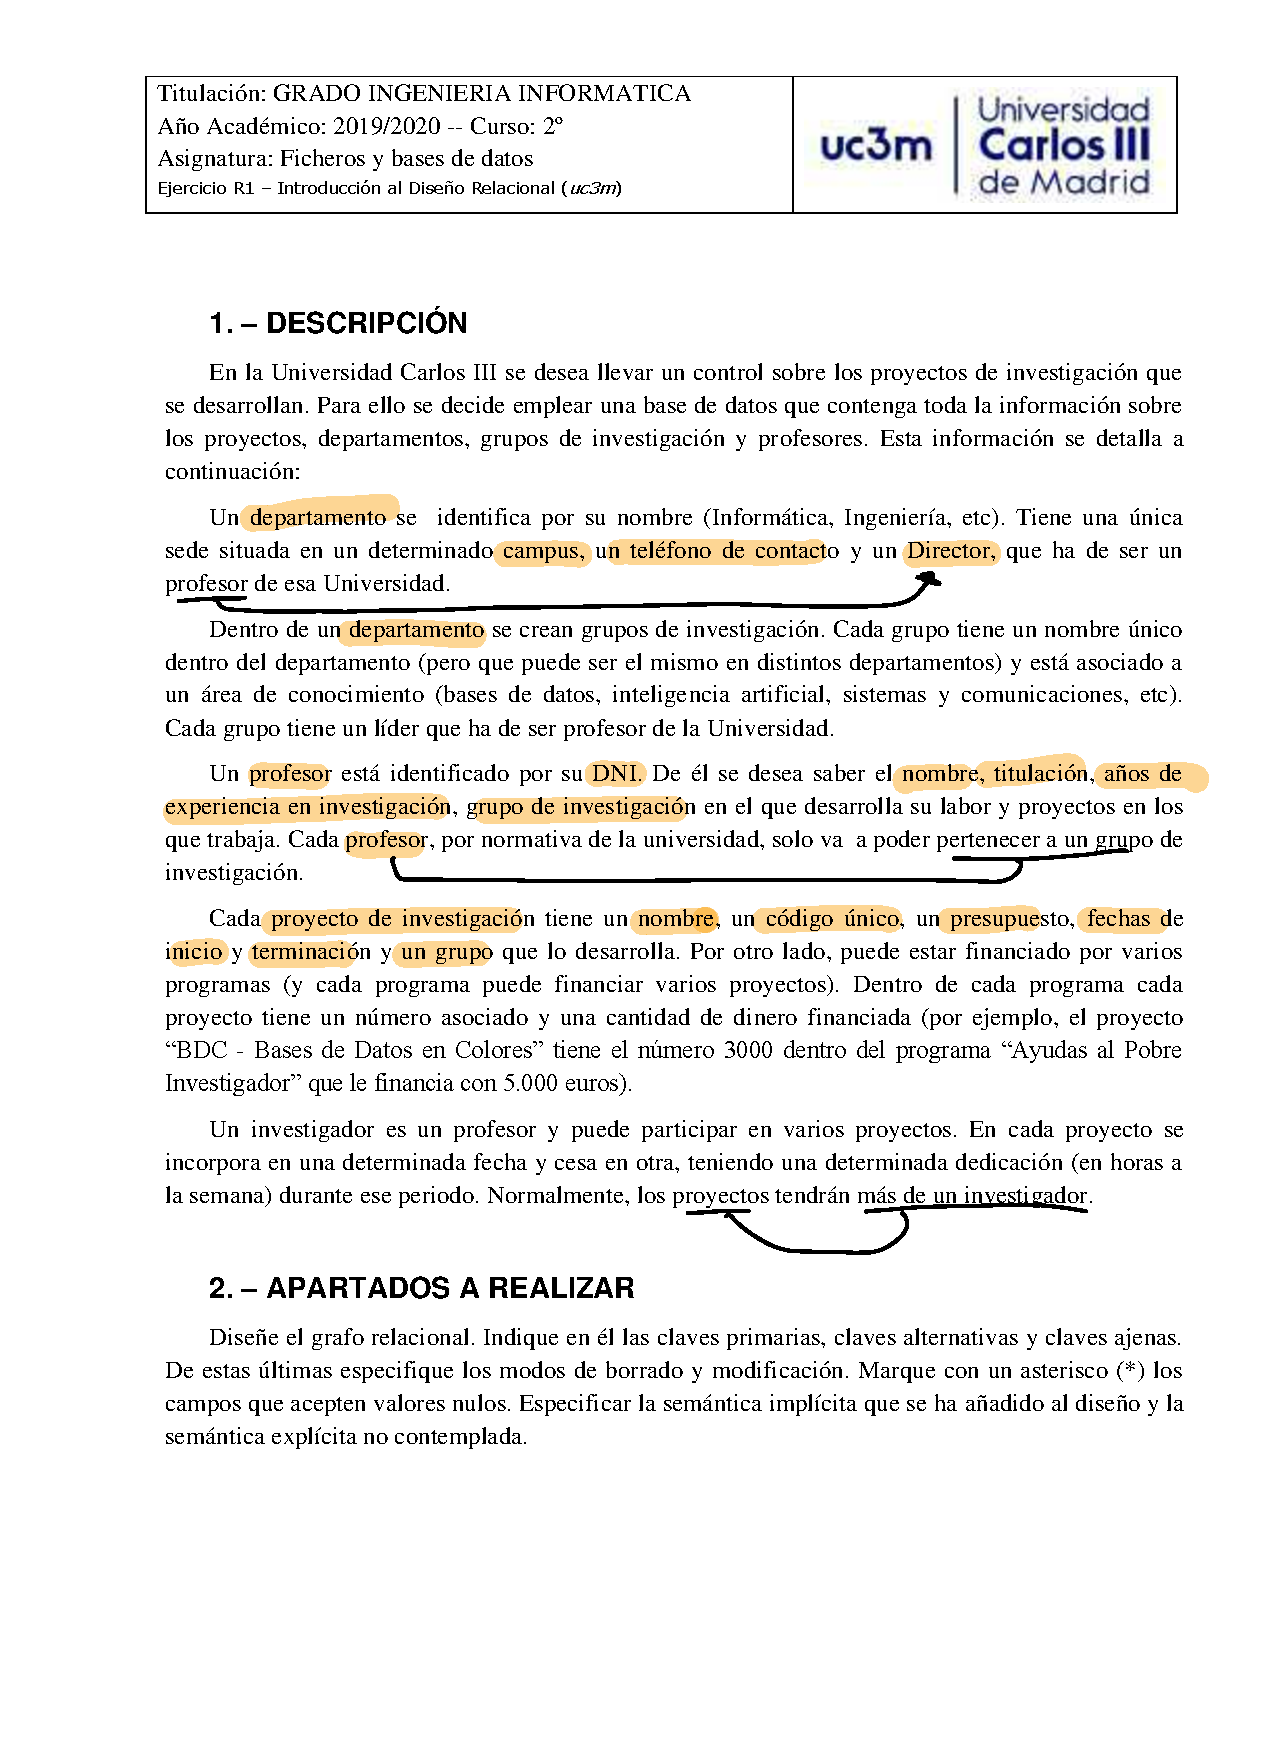
\includepdf[pages=-]{docs/Modelo_Racional_1.pdf}
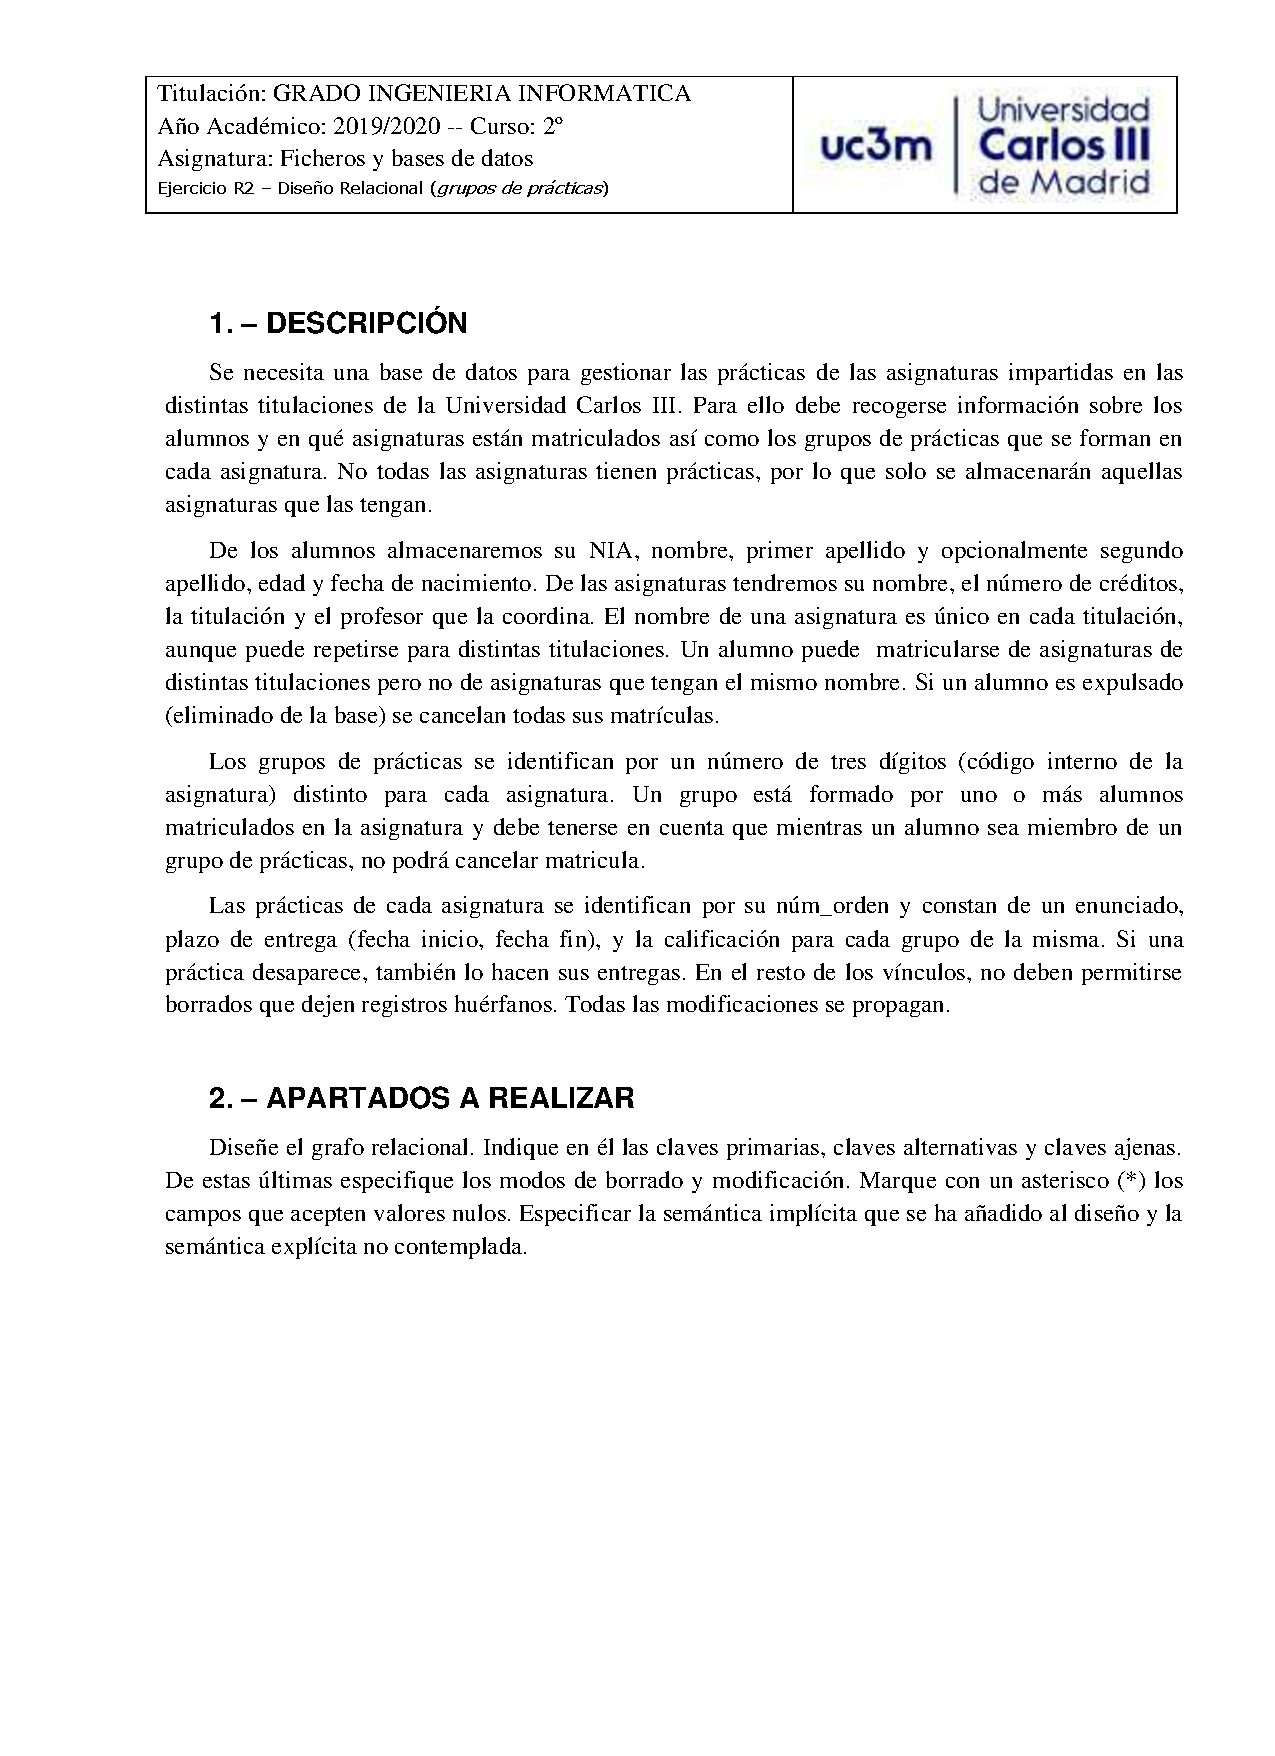
\includepdf[pages=-]{docs/Modelo_Racional_2.pdf}
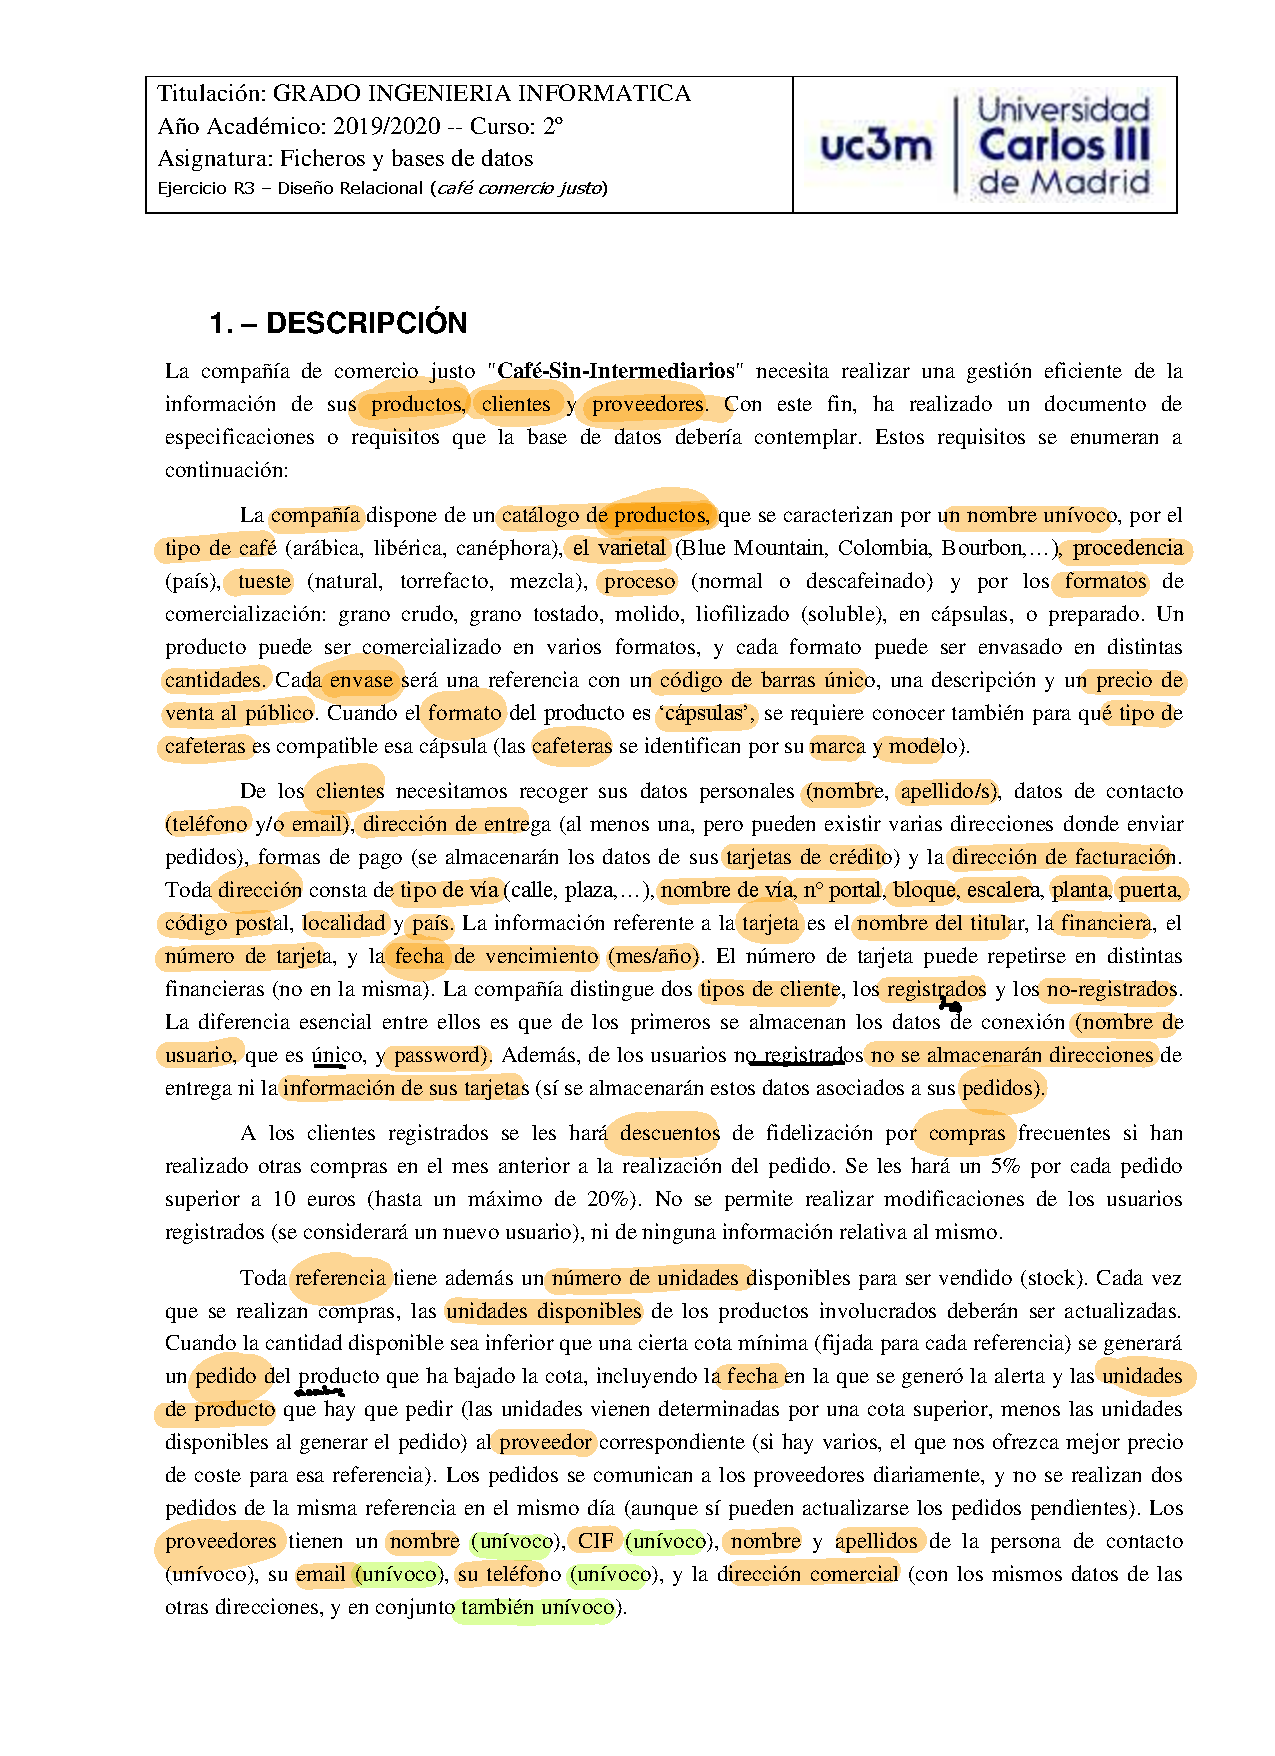
\includepdf[pages=-]{docs/Modelo_Racional_3.pdf}
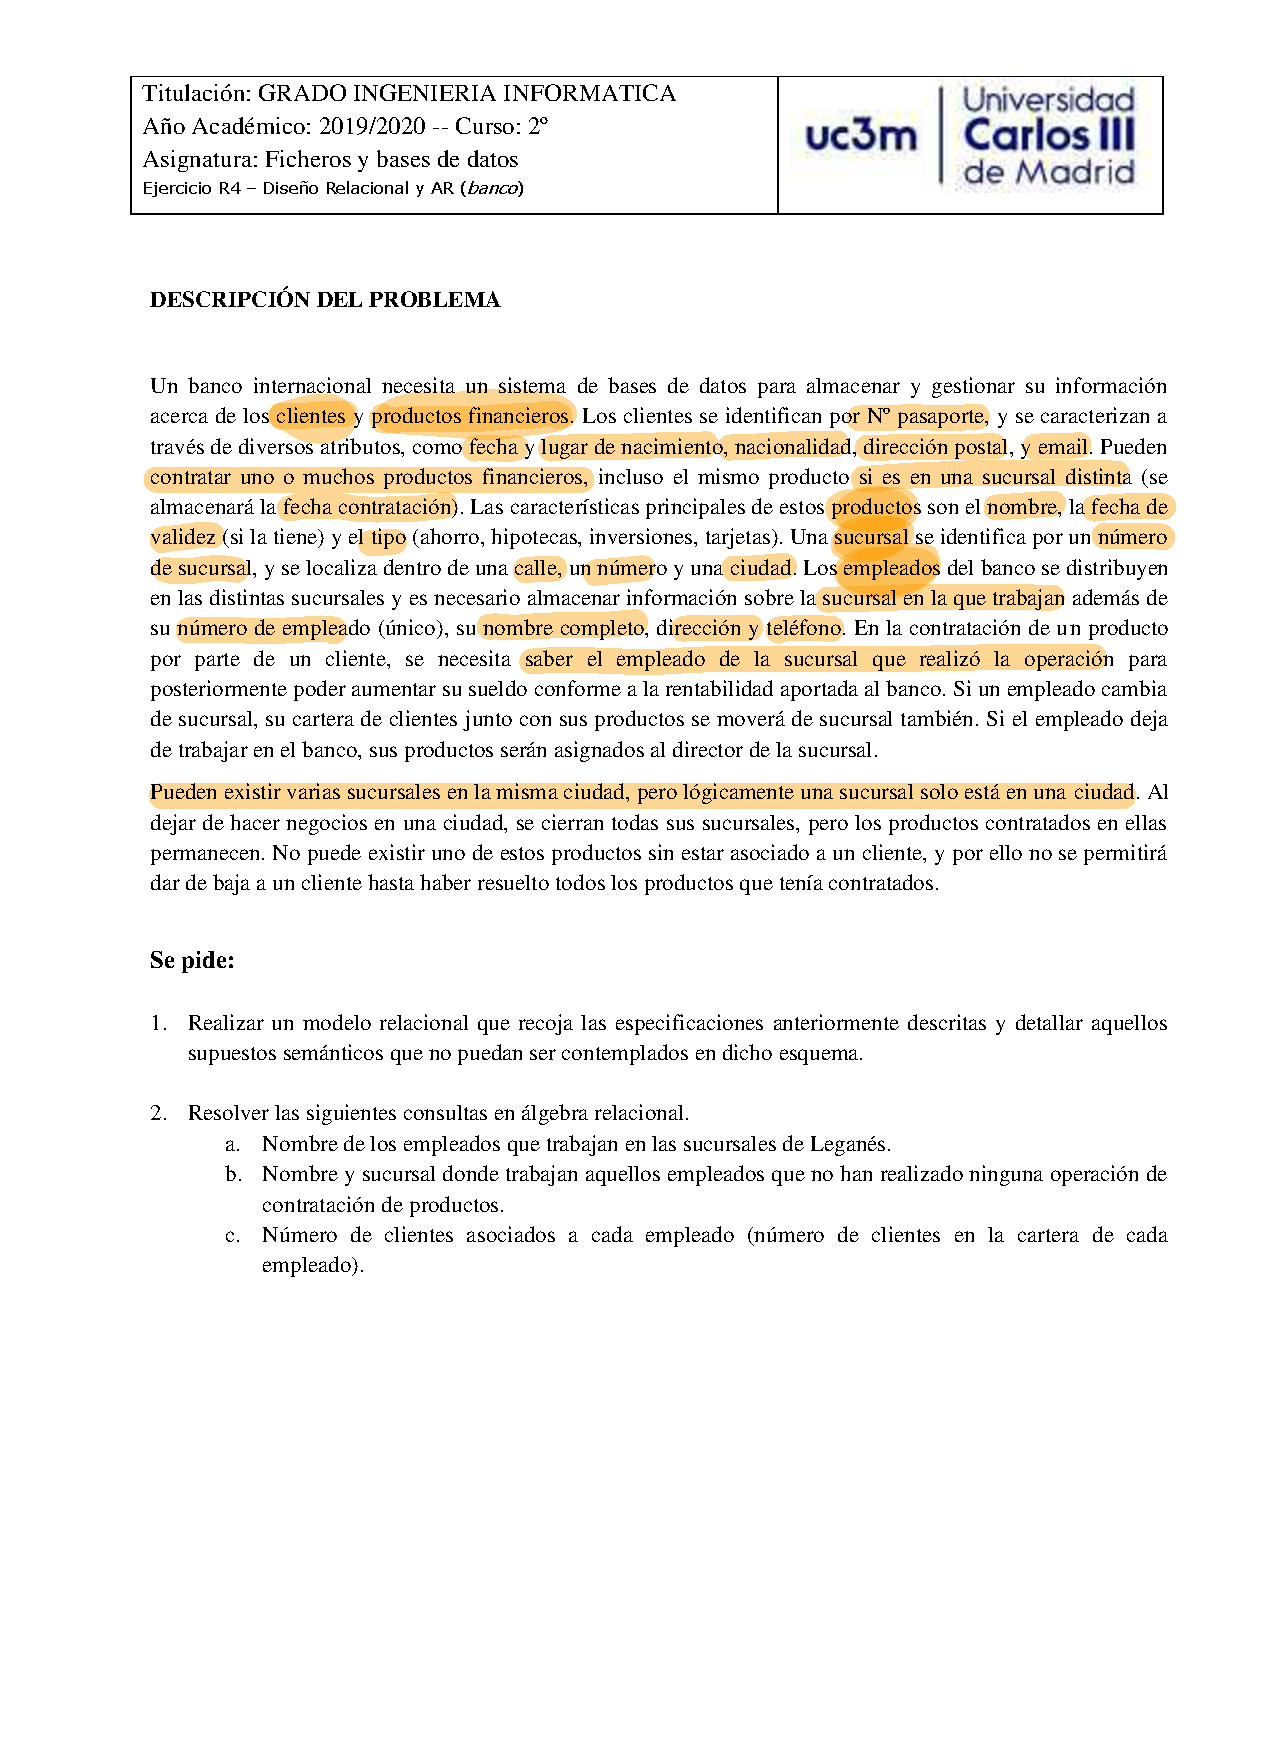
\includepdf[pages=-]{docs/Modelo_Racional_4.pdf}
\includepdf[pages=-]{docs/Modelo_Racional_6.pdf}
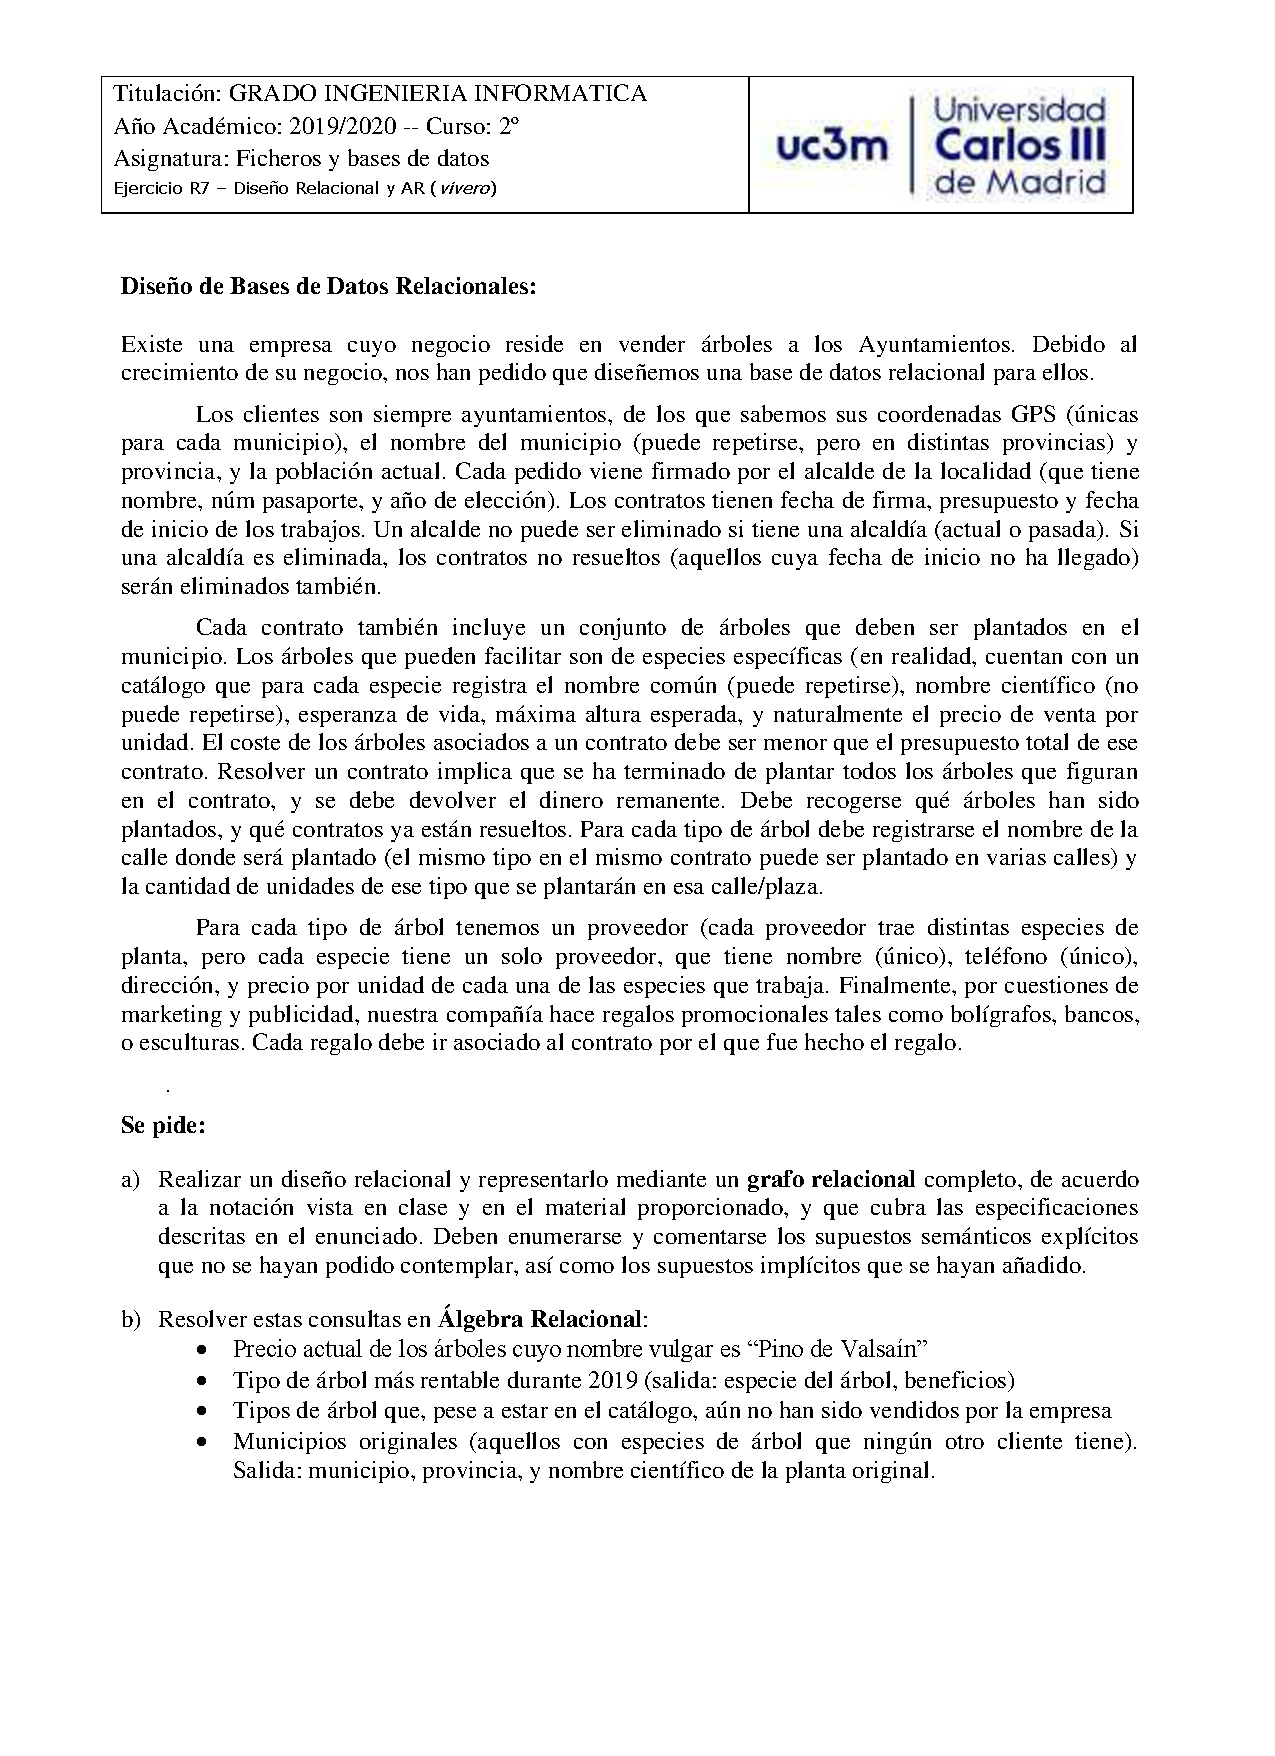
\includepdf[pages=-]{docs/Modelo_Racional_7.pdf}

\includepdf[pages=-]{docs/Modelo_Racional_8.pdf}
\includepdf[pages=-]{docs/repaso1.pdf}
\includepdf[pages=-]{docs/R1.pdf}
\includepdf[pages=-]{docs/R2esp.pdf}
\includepdf[pages=-]{docs/R4esp.pdf}
\includepdf[pages=-]{docs/R7esp.pdf}
\includepdf[pages=-]{docs/R8esp.pdf}
\includepdf[pages=-]{docs/Repaso_28-5.pdf}

\part{Práctica 1}
\includepdf[pages=-]{docs/100405834_100405951.pdf}
\includepdf[pages=-]{docs/2019-20-Enunciado_practica_1_comp.pdf}
\includepdf[pages=-]{docs/100405834_100405951.pdf}
\includepdf[pages=-]{docs/GI_FFBBDD_lab_I.pdf}
\includepdf[pages=-]{docs/GI_FFBBDD_lab_II.pdf}
\includepdf[pages=-]{docs/pract_sol.pdf}
\includepdf[pages=-]{docs/practica_1_2020.pdf}

\part{Práctica 2}
\includepdf[pages=-]{docs/FSDB_plantillaMemoria2.pdf}
\includepdf[pages=-]{docs/341ctica_2_def.pdf}
\includepdf[pages=-]{docs/ffesp.pdf}
\includepdf[pages=-]{docs/FSDB_Memoria2_100405951_100405834.pdf}

\part{Práctica 3}
\includepdf[pages=-]{docs/FSDB_Memoria_100405834_100405951.pdf}
\includepdf[pages=-]{docs/enunciado_P3_2020_esp.pdf}
\includepdf[pages=-]{docs/GI_FFBBDD_LW_IV.pdf}
\includepdf[pages=-]{docs/OPERATION_and_OPTIONS_Values_Produced_by_EXPLAIN_PLAN.pdf}

\part{Exámenes}
\includepdf[pages=-]{docs/100405951Ficheros1.pdf}
\includepdf[pages=-]{docs/ejercicio_2_2.pdf}
\includepdf[pages=-]{docs/100405951DisenoRelacional1.pdf}
\includepdf[pages=-]{docs/100405951DisenoRelacional2.pdf}
\includepdf[pages=-]{docs/100405951Ficheros.pdf}
\includepdf[pages=-]{docs/ej2_1.pdf}
\includepdf[pages=-]{docs/ejercicio_2_2.pdf}
\includepdf[pages=-]{docs/100405951DiseoRelacional1.pdf}
\includepdf[pages=-]{docs/100405951DisenoRelacional2.pdf}

\end{document}